%%%%%%%%%%%%%%%%%%%%%%%%%%%%%%%%%%%%%%%%%%%%%%%%%%%%%%%%%%%%%%%%%%%%%%
% Template for a UBC-compliant dissertation
% At the minimum, you will need to change the information found
% after the "Document meta-data"
%
%!TEX TS-program = pdflatex
%!TEX encoding = UTF-8 Unicode

%% The ubcdiss class provides several options:
%%   gpscopy (aka fogscopy)
%%       set parameters to exactly how GPS specifies
%%         * single-sided
%%         * page-numbering starts from title page
%%         * the lists of figures and tables have each entry prefixed
%%           with 'Figure' or 'Table'
%%       This can be tested by `\ifgpscopy ... \else ... \fi'
%%   10pt, 11pt, 12pt
%%       set default font size
%%   oneside, twoside
%%       whether to format for single-sided or double-sided printing
%%   balanced
%%       when double-sided, ensure page content is centred
%%       rather than slightly offset (the default)
%%   singlespacing, onehalfspacing, doublespacing
%%       set default inter-line text spacing; the ubcdiss class
%%       provides \textspacing to revert to this configured spacing
%%   draft
%%       disable more intensive processing, such as including
%%       graphics, etc.
%%

% For submission to GPS
\documentclass[gpscopy,onehalfspacing,11pt]{ubcdiss}

% For your own copies (looks nicer)
% \documentclass[balanced,twoside,11pt]{ubcdiss}

%%%%%%%%%%%%%%%%%%%%%%%%%%%%%%%%%%%%%%%%%%%%%%%%%%%%%%%%%%%%%%%%%%%%%%
%%%%%%%%%%%%%%%%%%%%%%%%%%%%%%%%%%%%%%%%%%%%%%%%%%%%%%%%%%%%%%%%%%%%%%
%%
%% FONTS:
%% 
%% The defaults below configures Times Roman for the serif font,
%% Helvetica for the sans serif font, and Courier for the
%% typewriter-style font.  Configuring fonts can be time
%% consuming; we recommend skipping to END FONTS!
%% 
%% If you're feeling brave, have lots of time, and wish to use one
%% your platform's native fonts, see the commented out bits below for
%% XeTeX/XeLaTeX.  This is not for the faint at heart. 
%% (And shouldn't you be writing? :-)
%%

%% NFSS font specification (New Font Selection Scheme)
\usepackage{times,mathptmx,courier}
\usepackage[scaled=.92]{helvet}

%% Math or theory people may want to include the handy AMS macros
\usepackage{amssymb}
\usepackage{amsmath}
\usepackage{amsfonts}

\usepackage{tikz}
\usetikzlibrary{patterns,shapes,backgrounds,shapes,positioning,petri,topaths,cd}

\usepackage[percent]{overpic}

%% The pifont package provides access to the elements in the dingbat font.   
%% Use \ding{##} for a particular dingbat (see p7 of psnfss2e.pdf)
%%   Useful:
%%     51,52 different forms of a checkmark
%%     54,55,56 different forms of a cross (saltyre)
%%     172-181 are 1-10 in open circle (serif)
%%     182-191 are 1-10 black circle (serif)
%%     192-201 are 1-10 in open circle (sans serif)
%%     202-211 are 1-10 in black circle (sans serif)
%% \begin{dinglist}{##}\item... or dingautolist (which auto-increments)
%% to create a bullet list with the provided character.
\usepackage{pifont}

%%%%%%%%%%%%%%%%%%%%%%%%%%%%%%%%%%%%%%%%%%%%%%%%%%%%%%%%%%%%%%%%%%%%%%
%% Configure fonts for XeTeX / XeLaTeX using the fontspec package.
%% Be sure to check out the fontspec documentation.
%\usepackage{fontspec,xltxtra,xunicode}	% required
%\defaultfontfeatures{Mapping=tex-text}	% recommended
%% Minion Pro and Myriad Pro are shipped with some versions of
%% Adobe Reader.  Adobe representatives have commented that these
%% fonts can be used outside of Adobe Reader.
%\setromanfont[Numbers=OldStyle]{Minion Pro}
%\setsansfont[Numbers=OldStyle,Scale=MatchLowercase]{Myriad Pro}
%\setmonofont[Scale=MatchLowercase]{Andale Mono}

%% Other alternatives:
%\setromanfont[Mapping=tex-text]{Adobe Caslon}
%\setsansfont[Scale=MatchLowercase]{Gill Sans}
%\setsansfont[Scale=MatchLowercase,Mapping=tex-text]{Futura}
%\setmonofont[Scale=MatchLowercase]{Andale Mono}
%\newfontfamily{\SYM}[Scale=0.9]{Zapf Dingbats}
%% END FONTS
%%%%%%%%%%%%%%%%%%%%%%%%%%%%%%%%%%%%%%%%%%%%%%%%%%%%%%%%%%%%%%%%%%%%%%
%%%%%%%%%%%%%%%%%%%%%%%%%%%%%%%%%%%%%%%%%%%%%%%%%%%%%%%%%%%%%%%%%%%%%%



%%%%%%%%%%%%%%%%%%%%%%%%%%%%%%%%%%%%%%%%%%%%%%%%%%%%%%%%%%%%%%%%%%%%%%
%%%%%%%%%%%%%%%%%%%%%%%%%%%%%%%%%%%%%%%%%%%%%%%%%%%%%%%%%%%%%%%%%%%%%%
%%
%% Recommended packages
%%
\usepackage{checkend}	% better error messages on left-open environments
\usepackage{graphicx}	% for incorporating external images

%% booktabs: provides some special commands for typesetting tables as used
%% in excellent journals.  Ignore the examples in the Lamport book!
\usepackage{booktabs}

%% listings: useful support for including source code listings, with
%% optional special keyword formatting.  The \lstset{} causes
%% the text to be typeset in a smaller sans serif font, with
%% proportional spacing.
\usepackage{listings}
\lstset{basicstyle=\sffamily\scriptsize,showstringspaces=false,fontadjust}

%% The acronym package provides support for defining acronyms, providing
%% their expansion when first used, and building glossaries.  See the
%% example in glossary.tex and the example usage throughout the example
%% document.
%% NOTE: to use \MakeTextLowercase in the \acsfont command below,
%%   we *must* use the `nohyperlinks' option -- it causes errors with
%%   hyperref otherwise.  See Section 5.2 in the ``LaTeX 2e for Class
%%   and Package Writers Guide'' (clsguide.pdf) for details.
\usepackage[printonlyused,nohyperlinks]{acronym}

\usepackage[sort=none]{glossaries-extra}
\glsenablehyper

%% The ubcdiss.cls loads the `textcase' package which provides commands
%% for upper-casing and lower-casing text.  The following causes
%% the acronym package to typeset acronyms in small-caps
%% as recommended by Bringhurst.
\renewcommand{\acsfont}[1]{{\scshape \MakeTextLowercase{#1}}}

%% color: add support for expressing colour models.  Grey can be used
%% to great effect to emphasize other parts of a graphic or text.
%% For an excellent set of examples, see Tufte's "Visual Display of
%% Quantitative Information" or "Envisioning Information".
\usepackage{color}
\definecolor{greytext}{gray}{0.5}


%\usepackage{subfloat}
\usepackage{subfig}


%% comment: provides a new {comment} environment: all text inside the
%% environment is ignored.
%%   \begin{comment} ignored text ... \end{comment}
\usepackage{comment}

%% The natbib package provides more sophisticated citing commands
%% such as \citeauthor{} to provide the author names of a work,
%% \citet{} to produce an author-and-reference citation,
%% \citep{} to produce a parenthetical citation.
%% We use \citeeg{} to provide examples
\usepackage[numbers,sort&compress]{natbib}
\newcommand{\citeeg}[1]{\citep[e.g.,][]{#1}}

%% The titlesec package provides commands to vary how chapter and
%% section titles are typeset.  The following uses more compact
%% spacings above and below the title.  The titleformat that follow
%% ensure chapter/section titles are set in singlespace.
\usepackage[compact]{titlesec}
\titleformat*{\section}{\singlespacing\raggedright\bfseries\Large}
\titleformat*{\subsection}{\singlespacing\raggedright\bfseries\large}
\titleformat*{\subsubsection}{\singlespacing\raggedright\bfseries}
\titleformat*{\paragraph}{\singlespacing\raggedright\itshape}

%% The caption package provides support for varying how table and
%% figure captions are typeset.
\usepackage[format=hang,indention=-1cm,labelfont={bf},margin=1em]{caption}

%% url: for typesetting URLs and smart(er) hyphenation.
%% \url{http://...} 
\usepackage{url}
\urlstyle{sf}	% typeset urls in sans-serif

\usepackage{siunitx} % Required for alignment
\sisetup{
	round-mode          = places, % Rounds numbers
	round-precision     = 2, % to 2 places
}

\usepackage{multirow} % Required for multirows

\usepackage{array,xcolor,colortbl}

%%%%%%%%%%%%%%%%%%%%%%%%%%%%%%%%%%%%%%%%%%%%%%%%%%%%%%%%%%%%%%%%%%%%%%
%%%%%%%%%%%%%%%%%%%%%%%%%%%%%%%%%%%%%%%%%%%%%%%%%%%%%%%%%%%%%%%%%%%%%%
%%
%% Possibly useful packages: you may need to explicitly install
%% these from CTAN if they aren't part of your distribution;
%% teTeX seems to ship with a smaller base than MikTeX and MacTeX.
%%
%\usepackage{pdfpages}	% insert pages from other PDF files
%\usepackage{longtable}	% provide tables spanning multiple pages
%\usepackage{chngpage}	% support changing the page widths on demand
\usepackage{tabularx}	% an enhanced tabular environment

%% enumitem: support pausing and resuming enumerate environments.
%\usepackage{enumitem}

%% rotating: provides two environments, sidewaystable and sidewaysfigure,
%% for typesetting tables and figures in landscape mode.  
%\usepackage{rotating}

%% subfig: provides for including subfigures within a figure,
%% and includes being able to separately reference the subfigures.
%\usepackage{subfig}

%% ragged2e: provides several new new commands \Centering, \RaggedLeft,
%% \RaggedRight and \justifying and new environments Center, FlushLeft,
%% FlushRight and justify, which set ragged text and are easily
%% configurable to allow hyphenation.
%\usepackage{ragged2e}

%% The ulem package provides a \sout{} for striking out text and
%% \xout for crossing out text.  The normalem and normalbf are
%% necessary as the package messes with the emphasis and bold fonts
%% otherwise.
%\usepackage[normalem,normalbf]{ulem}    % for \sout

%%%%%%%%%%%%%%%%%%%%%%%%%%%%%%%%%%%%%%%%%%%%%%%%%%%%%%%%%%%%%%%%%%%%%%
%% HYPERREF:
%% The hyperref package provides for embedding hyperlinks into your
%% document.  By default the table of contents, references, citations,
%% and footnotes are hyperlinked.
%%
%% Hyperref provides a very handy command for doing cross-references:
%% \autoref{}.  This is similar to \ref{} and \pageref{} except that
%% it automagically puts in the *type* of reference.  For example,
%% referencing a figure's label will put the text `Figure 3.4'.
%% And the text will be hyperlinked to the appropriate place in the
%% document.
%%
%% Generally hyperref should appear after most other packages

%% The `pagebackref' causes the references in the bibliography to have
%% back-references to the citing page; `backref' puts the citing section
%% number.  See further below for other examples of using hyperref.
%% 2009/12/09: now use `linktocpage' (Jacek Kisynski): GPS now prefers
%%   that the ToC, LoF, LoT place the hyperlink on the page number,
%%   rather than the entry text.
\ifgpscopy
  % GPS requires that weblinks should be dark blue, which looks a bit
  % odd in printed form.
  % https://www.grad.ubc.ca/current-students/dissertation-thesis-preparation/fonts-print
  \usepackage[bookmarks,bookmarksnumbered,%
     pagebackref,linktocpage,%
     colorlinks=true,%
     linkcolor=black,%
     urlcolor=blue,%
     citecolor=black%
     ]{hyperref}
\else
  %% The following puts hyperlinks in very faint grey boxes (in pdf only).
  \usepackage[bookmarks,bookmarksnumbered,%
    pagebackref,linktocpage,%
    allbordercolors={0.8 0.8 0.8},%
    ]{hyperref}
\fi
%% The following change how the the back-references text is typeset in a
%% bibliography when `backref' or `pagebackref' are used
%%
%% Change \nocitations if you'd like some text shown where there
%% are no citations found (e.g., pulled in with \nocite{xxx})
\newcommand{\nocitations}{\relax}
%%\newcommand{\nocitations}{No citations}
%%
%\renewcommand*{\backref}[1]{}% necessary for backref < 1.33
\renewcommand*{\backrefsep}{,~}%
\renewcommand*{\backreftwosep}{,~}% ', and~'
\renewcommand*{\backreflastsep}{,~}% ' and~'
\renewcommand*{\backrefalt}[4]{%
\textcolor{greytext}{\ifcase #1%
\nocitations%
\or
\(\rightarrow\) page #2%
\else
\(\rightarrow\) pages #2%
\fi}}


%% The following uses most defaults, which causes hyperlinks to be
%% surrounded by colourful boxes; the colours are only visible in
%% PDFs and don't show up when printed:
%\usepackage[bookmarks,bookmarksnumbered]{hyperref}

%% The following disables the colourful boxes around hyperlinks.
%\usepackage[bookmarks,bookmarksnumbered,pdfborder={0 0 0}]{hyperref}

%% The following disables all hyperlinking, but still enabled use of
%% \autoref{}
%\usepackage[draft]{hyperref}

%% The following commands causes chapter and section references to
%% uppercase the part name.
\renewcommand{\chapterautorefname}{Chapter}
\renewcommand{\sectionautorefname}{Section}
\renewcommand{\subsectionautorefname}{Section}
\renewcommand{\subsubsectionautorefname}{Section}

%% If you have long page numbers (e.g., roman numbers in the 
%% preliminary pages for page 28 = xxviii), you might need to
%% uncomment the following and tweak the \@pnumwidth length
%% (default: 1.55em).  See the tocloft documentation at
%% http://www.ctan.org/tex-archive/macros/latex/contrib/tocloft/
% \makeatletter
% \renewcommand{\@pnumwidth}{3em}
% \makeatother

%%%%%%%%%%%%%%%%%%%%%%%%%%%%%%%%%%%%%%%%%%%%%%%%%%%%%%%%%%%%%%%%%%%%%%
%%%%%%%%%%%%%%%%%%%%%%%%%%%%%%%%%%%%%%%%%%%%%%%%%%%%%%%%%%%%%%%%%%%%%%
%%
%% Some special settings that controls how text is typeset
%%
% \raggedbottom		% pages don't have to line up nicely on the last line
% \sloppy		% be a bit more relaxed in inter-word spacing
% \clubpenalty=10000	% try harder to avoid orphans
% \widowpenalty=10000	% try harder to avoid widows
% \tolerance=1000

%% And include some of our own useful macros
% This file provides examples of some useful macros for typesetting
% dissertations.  None of the macros defined here are necessary beyond
% for the template documentation, so feel free to change, remove, and add
% your own definitions.
%
% We recommend that you define macros to separate the semantics
% of the things you write from how they are presented.  For example,
% you'll see definitions below for a macro \file{}: by using
% \file{} consistently in the text, we can change how filenames
% are typeset simply by changing the definition of \file{} in
% this file.
% 
%% The following is a directive for TeXShop to indicate the main file
%%!TEX root = diss.tex

\newcommand{\NA}{\textsc{n/a}}	% for "not applicable"
\newcommand{\eg}{e.g.,\ }	% proper form of examples (\eg a, b, c)
\newcommand{\ie}{i.e.,\ }	% proper form for that is (\ie a, b, c)
\newcommand{\etal}{\emph{et al}}

% Some useful macros for typesetting terms.
\newcommand{\file}[1]{\texttt{#1}}
\newcommand{\class}[1]{\texttt{#1}}
\newcommand{\latexpackage}[1]{\href{http://www.ctan.org/macros/latex/contrib/#1}{\texttt{#1}}}
\newcommand{\latexmiscpackage}[1]{\href{http://www.ctan.org/macros/latex/contrib/misc/#1.sty}{\texttt{#1}}}
\newcommand{\env}[1]{\texttt{#1}}
\newcommand{\BibTeX}{Bib\TeX}

% Define a command \doi{} to typeset a digital object identifier (DOI).
% Note: if the following definition raise an error, then you likely
% have an ancient version of url.sty.  Either find a more recent version
% (3.1 or later work fine) and simply copy it into this directory,  or
% comment out the following two lines and uncomment the third.
\DeclareUrlCommand\DOI{}
\newcommand{\doi}[1]{\href{http://dx.doi.org/#1}{\DOI{doi:#1}}}
%\newcommand{\doi}[1]{\href{http://dx.doi.org/#1}{doi:#1}}

% Useful macro to reference an online document with a hyperlink
% as well with the URL explicitly listed in a footnote
% #1: the URL
% #2: the anchoring text
\newcommand{\webref}[2]{\href{#1}{#2}\footnote{\url{#1}}}

% epigraph is a nice environment for typesetting quotations
\makeatletter
\newenvironment{epigraph}{%
	\begin{flushright}
	\begin{minipage}{\columnwidth-0.75in}
	\begin{flushright}
	\@ifundefined{singlespacing}{}{\singlespacing}%
    }{
	\end{flushright}
	\end{minipage}
	\end{flushright}}
\makeatother

% \FIXME{} is a useful macro for noting things needing to be changed.
% The following definition will also output a warning to the console
\newcommand{\FIXME}[1]{\typeout{**FIXME** #1}\textbf{[FIXME: #1]}}

% END


%%%%%%%%%%%%%%%%%%%%%%%%%%%%%%%%%%%%%%%%%%%%%%%%%%%%%%%%%%%%%%%%%%%%%%
%%%%%%%%%%%%%%%%%%%%%%%%%%%%%%%%%%%%%%%%%%%%%%%%%%%%%%%%%%%%%%%%%%%%%%
%%
%% Document meta-data: be sure to also change the \hypersetup information
%%

\title{Augmenting Metadata Tags in Open Data Tables Using Schema Matching in a Pay-as-You-Go Fashion}
%\subtitle{If you want a subtitle}

\author{Haoran Yu}
\previousdegree{B.Sc., Computing Science, The University of British Columbia, 2017}
\previousdegree{B.Sc., Biochemistry, University of Toronto, 2014}

% What is this dissertation for?
\degreetitle{Master of Science}

\institution{The University of British Columbia}
\campus{Vancouver}

\faculty{The Faculty of Graduate and Postdoctoral Studies}
\department{Computer Science}
\submissionmonth{March}
\submissionyear{2023}

% details of your examining committee
\examiningcommittee{Rachel Pottinger, Computer Science, \textsc{UBC}}{Supervisor}
\examiningcommittee{Ed Knorr, Computer Science, \textsc{UBC}}{Examining Committee Member}
% details of your supervisory committee
%\supervisorycommittee{Rachel Pottinger, Professor,  Computer Science, \textsc{UBC}}%
%    {Supervisory Committee Member}

%% hyperref package provides support for embedding meta-data in .PDF
%% files
\hypersetup{
  pdftitle={Augmenting Metadata Tags in Open Data Tables Using Schema Matching in a Pay-as-You-Go Fashion},
  pdfauthor={Haoran Yu},
  pdfkeywords={Augmenting,Metadata,Schema,Matching}
}

%%%%%%%%%%%%%%%%%%%%%%%%%%%%%%%%%%%%%%%%%%%%%%%%%%%%%%%%%%%%%%%%%%%%%%
%%%%%%%%%%%%%%%%%%%%%%%%%%%%%%%%%%%%%%%%%%%%%%%%%%%%%%%%%%%%%%%%%%%%%%
%% 
%% The document content
%%

%% LaTeX's \includeonly commands causes any uses of \include{} to only
%% include files that are in the list.  This is helpful to produce
%% subsets of your thesis (e.g., for committee members who want to see
%% the dissertation chapter by chapter).  It also saves time by 
%% avoiding reprocessing the entire file.
%\includeonly{intro,conclusions}
%\includeonly{discussion}

\begin{document}

%%%%%%%%%%%%%%%%%%%%%%%%%%%%%%%%%%%%%%%%%%%%%%%%%%
%% From Thesis Components: Tradtional Thesis
%% <http://www.grad.ubc.ca/current-students/dissertation-thesis-preparation/order-components>

% Preliminary Pages (numbered in lower case Roman numerals)
%    1. Title page (mandatory)
\maketitle

%    2. Committee page (mandatory): lists supervisory committee and,
%    if applicable, the examining committee
\makecommitteepage

%    3. Abstract (mandatory - maximum 350 words)
%% The following is a directive for TeXShop to indicate the main file
%%!TEX root = diss.tex

\chapter{Abstract}
Metadata help users understand the data contents in the table, metadata tags can describe the contents in the table and allow a user to easily browse, search, and filter data. However, metadata is less useful due to heterogeneity and incompleteness in a table and its metadata. It's difficult to find all related tables to the given table by only examining the tags, because the user is typically looking for overlap of tags between two or more tables and there are no such overlaps in the heterogeneous metadata. We use Open Data tables in a case study, and develop strategies to augment the tags in table metadata to increase the tag overlaps between metadata of different tables. As an initialization step, we perform semantic enrichment of words in attributes of table schema and in tags, and perform schema matching between attributes and tags of a table to create semantic labeling, where an attribute is labeled with zero or more tags. We provide one base table, and search for tables using the semantic labeling we created to quickly find related tables. We integrated the table searching step and a schema matching step into an iterative framework, which incrementally add additional tags to a table’s metadata for all the tables related to the base table. The additional tags added to the metadata are discovered by semantics overlap during the schema matching step in the iterative framework, based on a composite score with evidence from multiple pairwise value comparison criteria. We evaluate two approaches we implemented using a gold standard we created, and compare the accuracy of the augmented tags and the runtime with two baseline approaches. We show that the tags augmented has a relatively high accuracy and the runtime of our iterative approach is reasonable. We argue that an approach that creates approximate matching in a pay-as-you-go fashion has a good precision and recall, and is the more realistic option in a real-world scenario.
\endinput
\cleardoublepage

%    4. Lay Summary (Effective May 2017, mandatory - maximum 150 words)
%% The following is a directive for TeXShop to indicate the main file
%%!TEX root = diss.tex

%% https://www.grad.ubc.ca/current-students/dissertation-thesis-preparation/preliminary-pages
%% 
%% LAY SUMMARY Effective May 2017, all theses and dissertations must
%% include a lay summary.  The lay or public summary explains the key
%% goals and contributions of the research/scholarly work in terms that
%% can be understood by the general public. It must not exceed 150
%% words in length.

\chapter{Lay Summary}

In large repositories where many tables are related to each other and each table containing rich data contents, there is usually not enough information to describe the contents of each table and how the tables are related to each other. Existing repositories use metadata of a table created by the authors to help users and computer programs to better understand the contents in the table, but it is often unable to fully describe the contents and the relatedness between tables. Open Data is one type of repository that exhibits such characteristics. We proposed approaches to solve the issue by augmenting existing metadata with additional tags such that more tags describe the contents of each table, and relatedness is captured by overlapping tags between tables. Our work is within the research area of heterogeneous metadata management for building data integration systems. Our work contributes improving the data-to-knowledge pipeline for big data.
\endinput
\cleardoublepage

%    5. Preface
%% The following is a directive for TeXShop to indicate the main file
%%!TEX root = diss.tex

\chapter{Preface}

This thesis is an original work of the author, Haoran Yu. The author designed the project, conducted all the experiments, and wrote the manuscript, under the supervision of Dr. Rachel Pottinger.
\endinput
\cleardoublepage

%    6. Table of contents (mandatory - list all items in the preliminary pages
%    starting with the abstract, followed by chapter headings and
%    subheadings, bibliographies and appendices)
\tableofcontents
\cleardoublepage	% required by tocloft package

%    7. List of tables (mandatory if thesis has tables)
\listoftables
\cleardoublepage	% required by tocloft package

%    8. List of figures (mandatory if thesis has figures)
\listoffigures
\cleardoublepage	% required by tocloft package

%    9. List of illustrations (mandatory if thesis has illustrations)
%   10. Lists of symbols, abbreviations or other (optional)

%   11. Glossary (optional)
%%% The following is a directive for TeXShop to indicate the main file
%%!TEX root = diss.tex

\chapter{Glossary}

This glossary uses the handy \latexpackage{acroynym} package to automatically
maintain the glossary.  It uses the package's \texttt{printonlyused}
option to include only those acronyms explicitly referenced in the
\LaTeX\ source.  To change how the acronyms are rendered, change the
\verb+\acsfont+ definition in \verb+diss.tex+.

% use \acrodef to define an acronym, but no listing
\acrodef{UI}{user interface}
\acrodef{UBC}{University of British Columbia}

% The acronym environment will typeset only those acronyms that were
% *actually used* in the course of the document
\begin{acronym}[ANOVA]
\acro{ANOVA}[ANOVA]{Analysis of Variance\acroextra{, a set of
  statistical techniques to identify sources of variability between groups}}
\acro{API}{application programming interface}
\acro{CTAN}{\acroextra{The }Common \TeX\ Archive Network}
\acro{DOI}{Document Object Identifier\acroextra{ (see
    \url{http://doi.org})}}
\acro{GPS}[GPS]{Graduate and Postdoctoral Studies}
\acro{PDF}{Portable Document Format}
\acro{RCS}[RCS]{Revision control system\acroextra{, a software
    tool for tracking changes to a set of files}}
\acro{TLX}[TLX]{Task Load Index\acroextra{, an instrument for gauging
  the subjective mental workload experienced by a human in performing
  a task}}
\acro{UML}{Unified Modelling Language\acroextra{, a visual language
    for modelling the structure of software artefacts}}
\acro{URL}{Unique Resource Locator\acroextra{, used to describe a
    means for obtaining some resource on the world wide web}}
\acro{W3C}[W3C]{\acroextra{the }World Wide Web Consortium\acroextra{,
    the standards body for web technologies}}
\acro{XML}{Extensible Markup Language}

\acro{data instance}{data in many shapes and formats, each data instance contains one table and metadata describing the data instance}
\acro{open data}{repository that contains a collection of data instances created and published by many individual authors, can be accessed by the general public without paying for the data}
\acro{metadata}{structured information about an information resource of any media type or format}

\acro{tag}{one type of metadata used in open data, it comes in the form of a list of one or more text items}
\acro{topic}{a tag that contains semantics such as a dictionary definition}
\acro{table}{a form of data instance, it is a two-dimensional matrix of values, where each column has a header}
\acro{header}{name of a column in a table}
\acro{schema}{metadata containing a list of mappings, where a header is mapped with a column}
\acro{attribute}{header within a schema}
\acro{constraint}{restrictions, for example, on the type of data stored in a column}
\acro{heterogeneity}{items that resemble the same information is represented differently across different data instances}
\acro{semantic heterogeneity}{the same data may have different meanings across different data instances (and vice versa)}
\acro{normalization}{ensure each data instance contains all the tags describing the same information}
\acro{metadata augmentation}{an approach to look for existing tags in the related tables, and for all tables lacking these tags, we add the tags to these tables}
\acro{semantic labeling}{matching between a set of attributes and a set of tags}
\acro{pay-as-you-go}{an approach where only the related tables are augmented with tags, and only tags that relates to the base table are augmented}
\acro{base table}{a table the user is familiar with its data and metadata}
\acro{word sense}{the meaning of a word, defined in a dictionary}
\acro{semantic enrichment}{the step to attach definitions to words}
\acro{word sense disambiguation}{the process of finding the correct interpretation of a word}
\acro{schema matching}{an algorithm that compare between a pair schemata, where attributes in one schema are compared to attributes of the second schema to find a matching}
\acro{matching criterion}{a function that determines the similarity between two attributes}
\acro{correspondence}{a pair from the matching in the form of (a,b,c), where a, b are attributes from the two schemata, and c is a score according to some matching criteria}
\acro{table searching}{an algorithm that searches the tables to find how tables are related, the query is compared with every other table in a pairwise manner}
\acro{ontology}{a collection of related concepts, each concept has a number of properties, and each concept is related to other concepts}
\acro{knowledge base}{a database storing a collection of facts that can be understood and processed by humans or machines}
\acro{data integration}{combining data instances by creating data mappings to capture the relatedness of attributes of the schemata}
\acro{mediated schema}{a schema with mediated attributes, where each schema has a source description (i.e., a mapping) in terms of the mediated schema}

\end{acronym}


% You can also use \newacro{}{} to only define acronyms
% but without explictly creating a glossary
% 
% \newacro{ANOVA}[ANOVA]{Analysis of Variance\acroextra{, a set of
%   statistical techniques to identify sources of variability between groups.}}
% \newacro{API}[API]{application programming interface}
% \newacro{GOMS}[GOMS]{Goals, Operators, Methods, and Selection\acroextra{,
%   a framework for usability analysis.}}
% \newacro{TLX}[TLX]{Task Load Index\acroextra{, an instrument for gauging
%   the subjective mental workload experienced by a human in performing
%   a task.}}
% \newacro{UI}[UI]{user interface}
% \newacro{UML}[UML]{Unified Modelling Language}
% \newacro{W3C}[W3C]{World Wide Web Consortium}
% \newacro{XML}[XML]{Extensible Markup Language}
\endinput	% always input, since other macros may rely on it

\newglossaryentry{attribute}{name=attribute:, description={another name for a column in a table}}
\newglossaryentry{base table}{name=base table:, description={a table the user is familiar with; its data and metadata}}
\newglossaryentry{constraint}{name=constraint:, description={restriction, for example, on the type of data stored in a column}}
\newglossaryentry{correspondence}{name=correspondence:, description={a triple from the match in the form ($a$, $b$, $c$), where $a$, $b$ are attributes from the two schemata, and $c$ is a score according to some matching criteria}}
\newglossaryentry{data instance}{name=data instance:, description={data has many shapes, sizes and formats; each data instance contains one table and its metadata}}
\newglossaryentry{data integration}{name=data integration:, description={the process of combining data instances by creating data mappings to capture the relatedness of attributes of the schemata}}
\newglossaryentry{header}{name=header:, description={name of a column in a table}}
\newglossaryentry{heterogeneity}{name=heterogeneity:, description={items that resemble the same information are represented differently across different data instances}}
\newglossaryentry{knowledge base}{name=knowledge base:, description={a database storing a collection of facts that can be understood and processed by humans or machines}}
\newglossaryentry{matching criterion}{name=matching criterion:, description={a function that determines the similarity between two attributes}}
\newglossaryentry{metadata}{name=metadata:, description={structured information about a resource of any media type or format; it describes the data}}
\newglossaryentry{metadata augmentation}{name=metadata augmentation:, description={an approach to look for existing tags in the related tables; and for all tables lacking these tags, we add the tags to these tables}}
\newglossaryentry{normalization}{name=normalization:, description={ensure each data instance contains all the tags describing the same information}}
\newglossaryentry{ontology}{name=ontology:, description={a collection of related concepts; each concept has a number of properties, and each concept is related to other concepts}}
\newglossaryentry{open data}{name=open data:, description={a repository that contains a collection of data instances created and published by many individual authors, and can be accessed by the general public without paying for the data}}
\newglossaryentry{pay-as-you-go}{name=pay-as-you-go:, description={an as-needed approach where only the related tables are augmented with tags; only tags that relate to the base table are augmented}}
\newglossaryentry{schema}{name=schema:, description={metadata containing a list of mappings, where a header is mapped to a column}}
\newglossaryentry{schema matching}{name=schema matching:, description={an algorithm to compare two schemata, where attributes in one schema are compared to attributes of the second schema to find a match}}
\newglossaryentry{semantic enrichment}{name=semantic enrichment:, description={the step to attach definitions to words}}
\newglossaryentry{semantic heterogeneity}{name=semantic heterogeneity:, description={the same data may have different meanings across different data instances (and vice versa)}}
\newglossaryentry{semantic labeling}{name=semantic labeling:, description={matching a set of attributes to a set of tags}}
\newglossaryentry{table}{name=table:, description={a form of data instance, it is a two-dimensional matrix of values, where each column has a header}}
\newglossaryentry{table searching}{name=table searching:, description={an algorithm that searches the tables to find how the tables are related; it compares the tables in a pairwise manner}}
\newglossaryentry{tag}{name=tag:, description={one type of metadata used in open data, it comes in the form of a list of one or more text items}}
\newglossaryentry{topic}{name=topic:, description={a tag that contains semantics such as a dictionary definition}}
\newglossaryentry{word sense}{name=word sense:, description={the meaning of a word, defined in a dictionary}}
\newglossaryentry{word sense disambiguation}{name=word sense disambiguation:, description={the process of finding the correct interpretation of a word}}


% \newglossarystyle{mystyle}{%
%  \setglossarystyle{treegroup}%
%  \renewcommand*{\glossentry}[2]{%
%    \glsentryitem{##1}\textbf{\glstarget{##1}{\glossentryname{##1}}}%
%    :\space \glossentrydesc{##1}\par
%  }%
% }

% \newglossarystyle
%  {mystyle}% style name
%  {% base it on the "list" style
%    \setglossarystyle{list}%
%    \renewcommand*{\glossentry}[2]{%
%      \item[\glsentryitem{##1}%
%           \glstarget{##1}{\glossentryname{##1}}]
%        \ifglshaslong{##1}%
%        { (\abbrtype{##1}: \glsentrylong{##1})\space}{}%
%        \glossentrydesc{##1}\glspostdescription\space ##2}%
%  }

 \newglossarystyle
 {mystyle}% style name
 {% base it on the "list" style
   \setglossarystyle{list}%
   \renewcommand*{\glossentry}[2]{%
     \item[\glsentryitem{##1}%
          \glstarget{##1}{\glossentryname{##1}}:]
       \ifglshaslong{##1}%
       { (\abbrtype{##1}: \glsentrylong{##1})\space}{}%
       \glossentrydesc{##1}\glspostdescription\space ##2}%
 }


\setglossarystyle{mystyle}

\printunsrtglossaries

\textspacing		% begin one-half or double spacing

%   12. Acknowledgements (optional)
%% The following is a directive for TeXShop to indicate the main file
%%!TEX root = diss.tex

\chapter{Acknowledgments}

I offer my enduring gratitude to Dr. Rachel Pottinger, whose inspiration, encouragement, and technical expertise helped me greatly in my studies. I also thank my fellow students Zainab Zolaktaf, Omar AlOmeir, Mostafa Milani, and Glenn Bevilacqua for their suggestions and mentorship in this field of research.

In addition, I am grateful to my second reader, Ed Knorr, for being my second reader, encouraging me to try research and make this thesis more complete.

Special thanks are owed to my parents, whose support throughout my years of education, both morally and financially, made me a confident individual capable of succeeding in my future endeavours.
\endinput

%   13. Dedication (optional)
%% The following is a directive for TeXShop to indicate the main file
%%!TEX root = diss.tex

\chapter{Dedication}

To my parents and grandparents.


% Body of Thesis (not all sections may apply)
\mainmatter

\acresetall	% reset all acronyms used so far


%    1. Introduction
%% The following is a directive for TeXShop to indicate the main file
%%!TEX root = diss.tex

\chapter{Introduction}
\label{ch:Introduction}

Storing and accessing information is one of the most important goals in computers. The data can be in many shapes and formats, and each of these  \acf{data instance} are collected into a repository. Open data is one such repository that contains a collection of data instances created and published by many individual authors, some of them government agencies. The rich repertoire of information in open data can be accessed by the general public without paying for the data. Along with the data instance itself, the repository also contains metadata for the data instance which can help someone to quickly understand what information is stored. Since each data instance stores different kinds of information, the metadata is very useful to describe and summarize the data stored, so that a user can browse a large number of data instances without too much effort trying to understand them. In general, the functions of metadata are explanation, summarization, and provenance \cite{10.1145/2845915}. The metadata can also help a user write queries on the data to answer his or her questions. The user or machine can easily perform searching and filtering that uses the metadata to group all the similar data into one place and access them together. At the same time, the metadata can aid machines to organize data, and track where the data came from, and link back to the original sources.

%%%%%%%%%%%%%%%%%%%%%%%%%%%%%%%%%%%%%%%%%%%%%%%%%%%%%%%%%%%%%%%%%%%%%%
\section{Definition of Metadata}
\label{sec:DefinitionOfMetadata}

Metadata is defined as “structured information about an information resource of any media type or format” \cite{Feltner2023Metadata}[20]. There are three types of metadata as explained in \cite{Baca2008}[3]: descriptive, administrative, and structural. Descriptive metadata tells what the data is about, administrative metadata stores information such as the intellectual property rights and use of information, and
structural metadata helps relate different data together. Tags is one type of metadata used in open data and its role is both descriptive and structural. It comes in the form of a list of one or more text items (each item is a word or phrase).

\subsection{Tags as metadata}

Tags can provide context for the data which allows someone to understand what the data is about without looking into the data itself. This is a good property as discussed by \cite{Wilkinson2016FAIR}[46]. With tags, the user can identify the intent of the data, determine its usefulness with respect to a given task, and take appropriate action. Tags can also help link different data instances together. If two data instances contain the same set of tags or overlap in many tags, then it is highly likely that the two data instances are similar and can be combined into a larger set of data.


%%%%%%%%%%%%%%%%%%%%%%%%%%%%%%%%%%%%%%%%%%%%%%%%%%%%%%%%%%%%%%%%%%%%%%
\section{Motivating example of tags}
\label{sec:MotivatingExampleOfTags}

We provide a motivating example from library studies, which emphasizes the usefulness of metadata. Journal articles are one type of data similar to open data; both are created and managed by different groups of authors. Each group manages a set of journal articles and is familiar with the contents of the articles, but the group is unfamiliar with articles managed by other groups. To aid a researcher to understand articles not managed by his or her group, metadata are tagged to each article. These metadata tags are usually created by the authors of the articles, and the purpose is to communicate with authors in other research groups who are interested in reading these articles. Once a researcher has read numerous articles with overlapping or similar tags, he or she is able to perform analysis, research, and generalize ideas from these articles.

%%%%%%%%%%%%%%%%%%%%%%%%%%%%%%%%%%%%%%%%%%%%%%%%%%%%%%%%%%%%%%%%%%%%%%
\section{The problems with anomalies in metadata}
\label{sec:TheProblemsWithAnomaliesInMetadata}

Open data was originally designed such that each data instance has complete and accurate data and metadata, which allows data in a repository to be more understandable and discoverable. However, in reality, many anomalies are present in the data and metadata. We focus on anomalies in the metadata. The metadata becomes less useful and misleading when it is incomplete, inaccurate, and heterogeneous.

\subsection{Incompleteness in metadata}
When the metadata does not contain complete information to summarize the contents of the data instance, it is insufficient to only look at the metadata to understand the underlying data. In the case of tags, the metadata for a data instance may contain some tags but it does not contain all of the tags needed to fully describe the data instance. The reason is that when an author creates tags for the data instance, he or she might only choose a few tags as metadata, and many other tags that could be useful are not included. When someone looks at the metadata of two related data instances, it might not be obvious that the two data instances contain related information because both of them only contain a few tags, and there are no overlaps between the two sets of tags.

\subsection{Inaccuracy in metadata}
Even if a data instance has rich metadata, the metadata may be inaccurate. For example, there may be spelling errors, typos, and formatting issues that prevents someone to interpret the metadata correctly. Even without errors, the tags may not be correctly chosen to describe the data instance.

\subsection{Heterogeneity in metadata}
There exists many types of heterogeneity in the metadata. In general, metadata items that resemble the same information might be represented differently across different data instances, and someone who do not know the different representations might not realize that the two metadata items are the same. Heterogeneities include mismatches in datatypes and differences in data granularities. With diverse data domains, each table is created for specific purposes, therefore the same data may have different meanings across different tables (and vice versa). This is known as semantic heterogeneity. A word can be represented using its synonyms, hypernyms, and acronyms, and resolving values that have the same meaning requires domain and technical expertise \cite{Halevy2005Why}[22].
In the case of metadata tags, many data instances share very similar data, but different data instances use different tags that are synonyms of each other. For example, the author of one journal article chooses a word as tag for the metadata, while an author of another journal article chooses a different word as tag for the metadata, without realizing that the two words are synonyms of each other. In the case of structured data instances (such as relational data), two attributes between two schemata represent the same information, but they use different attribute names.
A user may not find tags to be very useful when browsing or searching the tags due to the presence of heterogeneity. Someone who wants to read the two articles may only find one article relevant after looking at the metadata, because the tag words in the other article are unfamiliar to him or her. Without any technical expertise to resolve semantic heterogeneity, users need to
spend more time manually perform searching, filtering, and browsing to find related tables. Once related tables are found, it is also difficult to understand how one table is related to another.
Due to incompleteness, inaccuracy, and heterogeneity in the metadata, a user may not be able to understand the data by only browsing its metadata, and a machine cannot use metadata to perform searching and filtering.

%%%%%%%%%%%%%%%%%%%%%%%%%%%%%%%%%%%%%%%%%%%%%%%%%%%%%%%%%%%%%%%%%%%%%%
\section{Scope of study and resources}
\label{sec:ScopeOfStudyAndResources}

We study how to improve metadata with the anomalies discussed in \autoref{sec:TheProblemsWithAnomaliesInMetadata}, we will discuss a number of methods and their effectiveness. We first limit the scope of our study. To make the problem simpler and easier to explain, we only study open data in the form of tables, and only seek to improve the quantity of metadata in the form of tags. Data instances in other forms such as XML, spatial data, and images are not studied. Metadata in the form of sentences, schema, and constraints also exist in open data, but we do not aim to improve them. A number of terminologies are defined as follows.

\subsection{Terminologies and definitions}

\begin{itemize}
\item Let a table be a two-dimensional matrix of values, where each column has a header. Let the header be the name of a column.
\item Let metadata tags be a list of text items, where each text item may be a word or a phrase, but the text item may not be a sentence, XML, or data mapping.
\item We also make a distinction between tags and topics, where a tag is a text item without any semantics, but a topic contains semantics such as a dictionary definition. A category is a tag, but there is fewer (likely only one) such tags per table.
\item Let a schema be a form of metadata, containing a list of mappings, where a header is mapped with a column. We call the header an attribute of the schema. In the notation A.b, A is the name of the schema, and b is the name of the attribute within A.
\item Let constraints be restrictions, for example, on the type of data stored in a column (enforcing all values in a column must be integer). Foreign keys is another type of constraint, that restricts which two columns can be joined.
\item Finally, let each data instance in open data contain only one table, and the metadata describing the table. We may use data instance and table interchangeably, depending on the context of use.
\end{itemize}

%%%%%%%%%%%%%%%%%%%%%%%%%%%%%%%%%%%%%%%%%%%%%%%%%%%%%%%%%%%%%%%%%%%%%%
\section{Open data case study}
\label{sec:OpenDataCaseStudy}

\begin{figure}
    \centering
    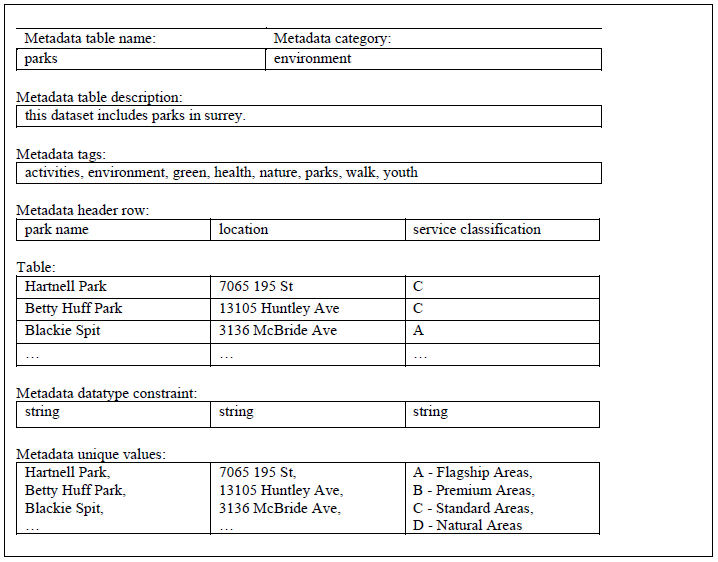
\includegraphics[width=5in]{figures/example-parks.png}
    \caption{Example data instance and metadata with table name parks}
    \label{fig:example-parks}
\end{figure}

We give examples of tables and metadata within an open data repository. We use City of Surrey Open Data1 as a case study. The metadata in this repository has many forms, such as the table name, the tags, the category the table belongs in, the header row of the tabular data, a paragraph in sentence form describing what information the table stores, the datatype constraint of each column, and the unique values in each column. Each metadata element either describes the entire table or a specific column of the table. \autoref{fig:example-parks} is an example of a table with its metadata. The table is the data instance containing data. The table name is parks. The table description informs that the table stores data for City of Surrey only. The category is environment; there may be other tables in the repository belonging in the same category. The tags list contains activities, environment, green, etc. The header row contains a list of column headers, such as the header park name for the first column of the table. For datatype constraint, the park name column is restricted to strings only, the other two columns are also restricted to strings. Values that are not the strings type do not appear in the column. The unique values contain example values of each column, such as ‘Hartnell Park’ for park name.
Each metadata form is simplified to be a list of text items. For example, a table name is a list containing one text item (one or more words), while the header row is a list of headers, and each header is a text item. The table description is also a list containing one text item.
The data instance such as the one in \autoref{fig:example-parks} can be represented more concisely for different purposes. The representation of a schema is:
Parks(park name, location, service classification)
where Parks is the name of the table (and the name of the schema), and park name, location, service classification are the attributes of the schema.
Similarly, the tags of the data instance is represented as:
Parks: {activities, environment, green, health, nature, parks, walk, youth}
where activities, environment, green, health, nature, parks, walk, youth, are the tags in the metadata of Parks.

\autoref{fig:example-park-specimen-trees}, \autoref{fig:example-drainage-catch-basins}, \autoref{fig:example-park-screen-trees}, and \autoref{fig:example-park-structures} are other examples of a table with its metadata.

\begin{figure}
    \centering
    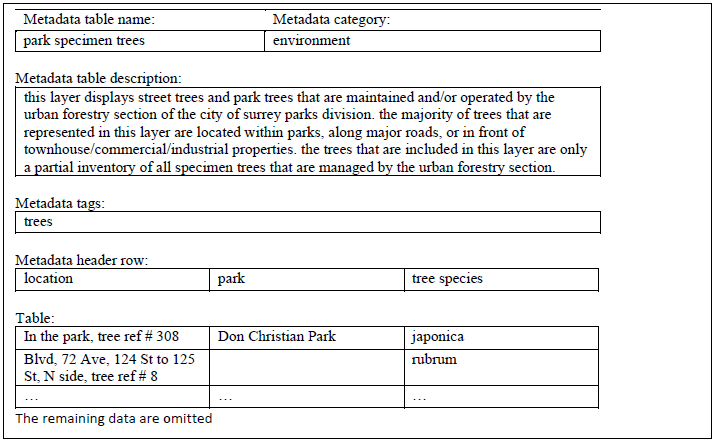
\includegraphics[width=5in]{figures/example-park-specimen-trees.png}
    \caption{Example data instance and metadata with table name park specimen trees}
    \label{fig:example-park-specimen-trees}
\end{figure}

\begin{figure}
    \centering
    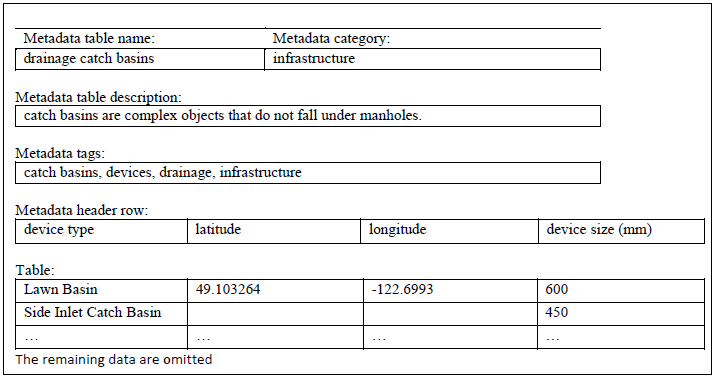
\includegraphics[width=5in]{figures/example-drainage-catch-basins.png}
    \caption{Example data instance and metadata with table name drainage catch basins}
    \label{fig:example-drainage-catch-basins}
\end{figure}

\begin{figure}
    \centering
    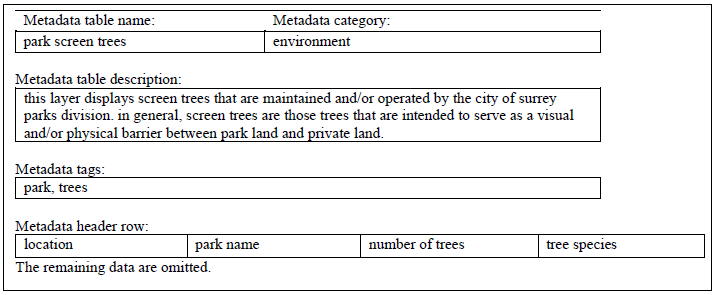
\includegraphics[width=5in]{figures/example-park-screen-trees.png}
    \caption{Example data instance and metadata with table name park screen trees}
    \label{fig:example-park-screen-trees}
\end{figure}

\begin{figure}
    \centering
    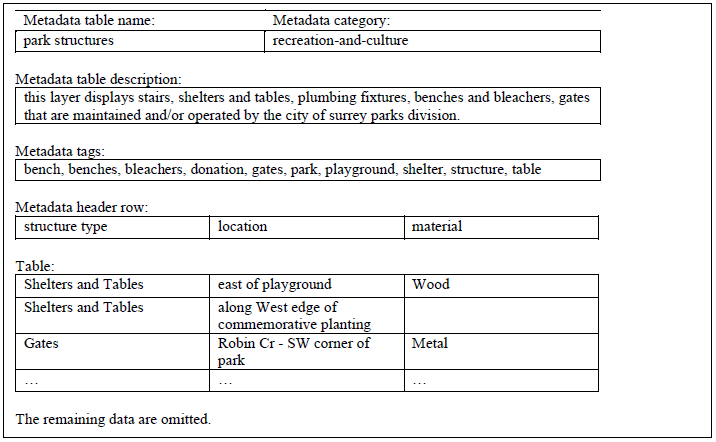
\includegraphics[width=5in]{figures/example-park-structures.png}
    \caption{Example data instance and metadata with table name park structures}
    \label{fig:example-park-structures}
\end{figure}

\subsection{Usefulness of header row in metadata}
We discuss what questions can be answered using the existing metadata in Surrey Open Data. When the table is available without any header row or any other metadata, it might not be clear what each of the values mean in the table. In \autoref{fig:example-parks}, the letters ‘C’ and ‘A’ in the third column could be interpreted in many ways. The letter might be the first letter of a word, or it might be a letter used for enumerating different classes. When the header row is present, each column is given more information to clarify what the column is about, but there is not enough information to interpret the values in the column. In \autoref{fig:example-parks}, the third column has the header service classification, which clarifies that the letters ‘C’ and ‘A’ are two service classes. But the header still does not inform what services ‘C’ and ‘A’ are.
If the user wants to join the two data instances in \autoref{fig:example-parks} and \autoref{fig:example-park-specimen-trees}, it is possible to join by location since both tables have a column with the header location. The user would find it much easier if they have access to the header rows when they first obtained the data instances. The header row allows the user to quickly find potential overlapping columns, and save time by not examining every column in the data instances. Although the header row itself is not informative enough to determine if two columns are joinable, it is still a good approximation. When the user sees two columns with a common header, the user is more likely to spend more time on the tables to investigate.

\subsection{Usefulness of unique values in metadata}

The unique values contains all possible values in a column. If the values in the column are abbreviations or symbols, unique values contains the full words for the abbreviations or symbols.
When the metadata is provided to each column, we can further decode the meaning of each value in a column. In \autoref{fig:example-parks}, values in the third column ‘C’ and ‘A’ are two classes of services, and the unique values decodes ‘C’ to ‘Standard Areas’ and ‘A’ to ‘Flagship Areas’.

\subsection{Usefulness of tags in metadata}
Given some tables in a repository, the user would like to find out which tables are relevant to some tasks, and by using the metadata tags the user can quickly filter out irrelevant tables. In \autoref{fig:example-park-specimen-trees}, the table name is park specimen trees and the only tag is trees. In \autoref{fig:example-park-screen-trees}, the table name is park screen trees and its tags are park and trees. Without looking into the values of the table instances, the user can quickly identify that both table instances contain some metadata about trees, and if the user is interested in studying trees, then both tables should be selected for further analysis. On the other hand, if the table name is drainage catch basins and the tags are devices and infrastructure, then the user should filter out the table immediately since the metadata does not seem to store any information about trees.
The idea of tag overlaps also applies to searching by machines. Using \autoref{fig:example-parks} and \autoref{fig:example-park-screen-trees} as an example, if the word park is a search keyword, then both tables will be returned as results of the search, since both contain the word park in the metadata tags. But if the search is on park AND trees to search for information about trees in parks, then the metadata of the tables need to overlap in both park and trees in order to show up in the search result. Only the second table is returned in the search result because it overlaps in both tags. Note that it is evident from the table description that the word park is interpreted as open green spaces.

%%%%%%%%%%%%%%%%%%%%%%%%%%%%%%%%%%%%%%%%%%%%%%%%%%%%%%%%%%%%%%%%%%%%%%
\section{Causes of anomalies in open data}
\label{sec:CausesOfAnomaliesInOpenData}

As discussed by \cite{10.1145/2845915}[1], present-day data management faces challenges in the aspects of volume, velocity, and variety. We will explain these challenges in the context of our study of open data and how they caused the anomalies in the data and metadata we discussed in \autoref{sec:TheProblemsWithAnomaliesInMetadata}.
Since the volume of some data collection is too large to be stored at one single location, and needs to be distributed to multiple locations, these data cannot be managed by one user. In open data repositories, there may be many attributes between schemata with complex relationships between them. However, it is difficult to discover these complex relationships when data are distributed.
Data grows at a very high velocity and is constantly changing, thus the users are required to constantly receive updates on the newest data. Managing the changing data also becomes difficult, and each of the tables becomes poor in quality because data values and metadata for tables are getting incomplete and inaccurate.
Due to the large volume of data and the rate that they are changing, it is inevitable that the data standards become out of sync where each individual user invents his or her own standards for maintaining the data that they have direct access to. Each user is able to maintain high quality for the data and metadata of their tables, but over time, the degree of heterogeneity between the data instances increases, which prevents one user to understand another user’s data instance due to differences in constraints, data granularities, naming convention, and representation. If the different data instances did not belong in the same data domain initially, the difficulty to communicate information between the data instances can only be greater.

\subsection{Open data common anomalies}
In Surrey Open Data, tables show many data anomalies, and we will give examples to each anomaly. Looking at \autoref{fig:example-park-specimen-trees}, we see that there is a missing value in the second row in the column with header park. When a table contains missing values, it is less likely for someone to correctly interpret the values in the table. When reading the table row by row, some rows may not make much sense due to missing some important values.
There are spelling errors or formatting inconsistencies in the table values. In \autoref{fig:example-park-specimen-trees}, values in the location column contain tree ref numbers, but some numbers are immediately preceded by a \verb+‘#’+ symbol while others have a \verb+‘#’+ followed by a space. Although the inconsistency is trivial to fix by hand for small table instances, it is more challenging if there are too many varieties of inconsistencies in many different tables and fixes can only be done programmatically. Many kinds of inconsistencies and spelling errors are difficult to detect, and if the fixes are done incorrectly, the values in the tables become even less interpretable.
Within each value, a user may find two or more kinds of information. In \autoref{fig:example-park-specimen-trees}, a value in the location column contains both the address as well as a reference number for the tree. To fix this issue, it is possible to move the reference number to a new column, and create a new header tree reference number for the new column.

Many abbreviations are used throughout the table instance in \autoref{fig:example-park-specimen-trees}. The word ‘ref’ is the abbreviation for ‘reference’, and ‘N’ is the abbreviation for ‘North’. While humans are able to interpret these abbreviations by observing the context that they are used, a program may not be able to interpret them if it cannot access the context.

Semantic heterogeneity is prevalent in the tables. The column with header park name in \autoref{fig:example-parks} and the column with header park in \autoref{fig:example-park-specimen-trees} seem to store the same kind of information, the names of parks. However, without inspecting the values in the tables, it is less likely for the user to conclude that these two columns store the same kind of information. At the same time, in the location columns of \autoref{fig:example-parks} and \autoref{fig:example-park-specimen-trees}, abbreviations such as Blvd, St, and Ave all refer to names of roads for vehicles, but if the user does not already have the domain knowledge, these abbreviations do not share any similarities.
The anomalies discussed above also occur in the metadata, but since metadata aims to provide more useful information to make the table more understandable, there are less abbreviations, less spelling errors, and more concise representation of information \cite{Rahm2016Case}[39]. However, metadata are more incomplete and heterogeneous due to the lack of effort creating them and maintaining them. In the case of \autoref{fig:example-park-specimen-trees}, the only tag in the metadata is trees, but tags such as park, species and urban should also be included to describe the table. The tag park has synonyms such as green and parkland, which should also be included in the metadata.

%%%%%%%%%%%%%%%%%%%%%%%%%%%%%%%%%%%%%%%%%%%%%%%%%%%%%%%%%%%%%%%%%%%%%%
\section{Scope of improving metadata}
\label{sec:ScopeOfImprovingMetadata}

There are many ways to improve the metadata and to fix the anomalies, but we are unable to discuss all of them. Our improvement is limited to the following scenario: a user is given a table he or she is familiar with, called a base table, and is given a number of tables in an open data repository. The user should be able to only look at the metadata to find all the related tables, and to get a sense of what data are stored in these tables. The user does not need to look at the contents in the tables to determine whether or not the two tables are similar.
It is often sufficient to show metadata that are related to the users goal. The user can understand the metadata more quickly because the unrelated metadata that could distract the user are not shown. If two tables overlap in a data domain of interest, then all metadata describing the data domain need to also overlap. If the two tables overlap in a data domain that is not related to a users goal, then overlaps in that data domain are not needed. Our work will be limited to improving metadata tags, we think tags are good summaries of the data contained in each table. Tags are machine-readable and can be processed by programs to perform keyword search or to compare between the tables.
To give an example, a user is interested in finding information about benches in parks, and finds one candidate table storing information about park structures of all types. In this table, there is a small portion of data storing benches in parks while the majority of data are about other information such as park gates and park tables. When we improve the metadata, we should only focus on improving metadata about benches, and ignore any additional metadata unrelated to


benches. Tables containing information about benches must contain the tag bench as well as tags related to benches, while the improved tags does not need to contain tags unrelated to benches.
When the metadata does not contain tags, the user would have to manually summarize the contents of a table, which would require additional time. We therefore only seek to provide a basic summary with the metadata, so that the user can save some time. Similarly, in the presence of metadata anomalies, the user would need to compare tables to find out all possible tags related to the base table, and needs to study tables separately one by one to obtain a complete view of all the metadata.

\subsection{Idea: normalizing metadata}
We outline our general approach to improve the metadata tags of tables in an open data repository. If there are two tags describing the same information, the user would want to add both tags to the metadata of all the tables containing this information. We seek all such tags, and ensure each table contains all the tags describing the same information. We call this procedure normalization of metadata tags. In other words, a tag is added to all the relevant tables.
The user can then use any of these tags to perform search on the repository and obtain all the tables related to the base table. To achieve normalization, we need to describe how the metadata between the different tables are related, we use a mapping (between an attribute and a tag) called semantic labeling to capture the relatedness.

The relatedness then allows the tables reach a consensus on the representation of tags for all the tags that they share in common, so that overlap is maximized. Our approach is called augmentation of metadata. We look for existing tags in the related tables, and for all tables lacking these tags, we add the tags to these tables. We also examine the existing tags of a table to find other tags that can be shared between a group of related tables, and for the tables that do not already contain some of these tags, we add the tags to the tables. Augmentation of metadata is done in an iterative manner, where tags are gradually added to the metadata of each table in many iterations. This metadata augmentation procedure is done in a pay-as-you-go fashion, where only the related tables are augmented with tags, and only tags that relates to the base table are augmented.
After the common representation of tags is found using normalization, tables with insufficient metadata is augmented with additional tags from a list of known tags. We show an example of the result of our automated metadata augmentation in \autoref{fig:augmented-park-specimen-trees}, using \autoref{fig:example-parks}, \autoref{fig:example-park-specimen-trees}, \autoref{fig:example-drainage-catch-basins}, \autoref{fig:example-park-screen-trees}, and \autoref{fig:example-park-structures} as our repository. In this example, additional tags for the

\begin{figure}
    \centering
    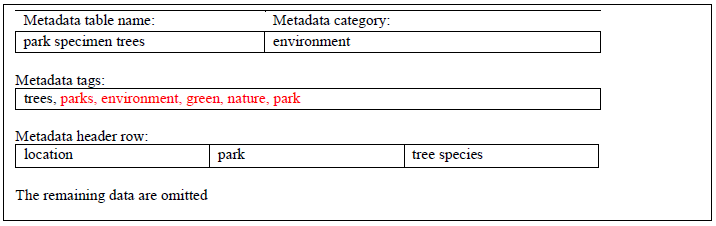
\includegraphics[width=5in]{figures/augmented-park-specimen-trees.png}
    \caption{Augmented tags of the table park specimen trees (shown in red)}
    \label{fig:augmented-park-specimen-trees}
\end{figure}

park specimen trees table are added to the metadata, regardless of whether park specimen trees is the base table. The additional tags originate from other tables in the repository.
To overcome semantic heterogeneity, we perform semantic enrichment (attaching a dictionary definition to each word) of the metadata. We use a domain dictionary to assist us with listing all possible interpretations of a word. We use a technique called word sense disambiguation (probabilistically assign definition to each word) to find a correct interpretation of a word. We then use an algorithm called schema matching to create the semantic labeling of tables (by probabilistically matching between attributes and tags). The output of schema matching, called the correspondences, serves as the key intermediate for semantic labeling. To find the relatedness between tables, we adopt a table searching algorithm that relies on the semantic labeling to find the maximum tag overlaps between tables.

%%%%%%%%%%%%%%%%%%%%%%%%%%%%%%%%%%%%%%%%%%%%%%%%%%%%%%%%%%%%%%%%%%%%%%
\section{Problem Definition}
\label{sec:ProblemDefinition}

We will now define our problem that we have introduced in \autoref{sec:ScopeOfStudyAndResources} and \autoref{sec:ScopeOfImprovingMetadata}. The input to our problem is a set of data instances, each containing a table, a metadata schema for the table, and a list of metadata text items describing the data instance. Each table contains a header row, and there is a column header for each table column. The text items may or may not be able to describe the table.

\subsection{Inputs and outputs}
\begin{itemize}
    \item 
\end{itemize}

More formally, let a data instance, s, consist of:
\begin{itemize}
\item A Table Ts , where Ts contains a header row that consists of column headers, but no type information
\item Let As be the attributes within the schema of Ts , where each attribute provides constraints for a header. We denote the attribute for the ith header in the header row of table Ts as Asi
\item Ls , a list of text items describing the contents of s , where Lsj is the jth text item in Ls
\end{itemize}
We take as input to our problem:
\begin{itemize}
\item A base data instance sq to be compared with other data instances
\item a set of k data instances, D, from unknown domains, which could be related to the sq . The correspondences between attributes of these data instances are unavailable. The semantic labeling is also unavailable.
\item A domain dictionary W , that can provide the semantics for values in Ts , As , and Ls
\end{itemize}
The outputs are:
\begin{itemize}
\item A set of data instances l  D related to sq, where l . k
\item A augmented list of L'sq such that L'sq more accurately describes the contents of sq
\item l augmented lists of L's such that L's more accurately describes the contents of s  D than Ls
\end{itemize}

\subsection{Assumptions}
Under the following assumptions, our solutions can be correctly implemented:

\begin{enumerate}
\item Each table contains a list of likely incomplete text items (metadata tags) describing the contents of the data instance. The list can be empty
\item The authors made an attempt at creating the metadata, it was not generated without inspection, therefore we trust the provided metadata
\item The goal of augmenting metadata tags for a table is for the user to get approximate answers quickly, but not precise answers. That is, metadata tags are augmented in a pay-as-you-go fashion
\item The user already knows what kinds of metadata is useful and interesting to look at, therefore we just have to augment tags that the user needs
\item All attributes in one schema are independent of one another. This assumption may not be true, but it is plausible and allows us to simplify our problem
\item The set of all topics in the repository are the only topics used for augmenting tables, that is, we do not create new topics that did not already exist in the repository. This assumption reduces a lot of uncertainty in our evaluations	
\end{enumerate}

%%%%%%%%%%%%%%%%%%%%%%%%%%%%%%%%%%%%%%%%%%%%%%%%%%%%%%%%%%%%%%%%%%%%%%
\section{Contributions}
\label{sec:Contributions}
The contributions we make in this thesis are the following:
\begin{enumerate}
\item We give a different perspective to the problem of augmenting tags in tables with incomplete metadata. We proposed an iterative approach, where given a base table with incomplete metadata, find other tables in the repository similar to the base table, and then iteratively find as much overlap between all related tables as possible.
\item We give a detailed explanation of why high-quality metadata can reveal new information to the user and how it can help organize existing data in a repository. We outlined that it is easy for users to navigate a repository, perform filter and search, and understand data and metadata of tables without looking at the values in the tables. Metadata tags also allows more automation in that they increase precision and recall for machine operations.
\item We discuss a number of techniques used to solve other problem, and we explain how these techniques can be applied to our problem.	
\end{enumerate}

The rest of this thesis is presented as follows. In \autoref{ch:RelatedWork}, we discuss a number of related fields of study and point out the strengths and weaknesses in solving our problem. In \autoref{ch:Preliminaries}, we provide detailed explanations of techniques that we used in our approach to augment metadata. In \autoref{ch:Solutions}, we discuss our proposed approaches as well as baseline approaches in solving the metadata augmentation problem. In \autoref{ch:Implementations}, we discuss how we implemented our approaches as well as the evaluations of our approaches. In \autoref{ch:Discussions}, we provide discussions of metadata augmentation and how it plays a role in data management research. We conclude in \autoref{ch:Conclusion}.


%    2. Related Work
%% The following is a directive for TeXShop to indicate the main file
%%!TEX root = diss.tex

\chapter{Related Work}
\label{ch:RelatedWork}

Augmenting metadata is considered an ill-defined field of study because of the lack of existing literatures that directly address the problem. But there are many other fields of study that target problems similar in nature. For example, we can relate our task to \textit{data discovery, topic extraction, summary generation,} and \textit{data integration}. Data discovery determines whether there is interesting information in some data, which allows relating seemingly unrelated data together. In topic extraction and summary generation, the end result is a concise and compact representation of information in a data instance, which is highly similar to the augmented tags. \textbf{\Gls{data integration}} plays important roles in creating common representation of data for different heterogeneous data instances, and combine the data from different data instances together.

Of all these problems, there are differences in the type of input data, output data, as well as intermediate steps that produces useful information. We therefore need to create abstractions of the different problems, break down large problems into smaller steps, and then identify the steps that we can reuse.

Of the four fields of study mentioned above, we first discuss data discovery in \autoref{sec:DataDiscovery}, where we specifically talk about \textit{information retrieval} and \textit{table linking}. We then discuss knowledge extraction and summary generation in \autoref{sec:KnowledgeExtractionAndSummaryGeneration}, where we specifically talk about \textit{topic modelling, ontology extraction,} and \textit{text summarization}. Finally, we talk about the various applications of data integration in \autoref{sec:DataIntegration}, and we briefly mention its relevance to \textit{data completion}.

%%%%%%%%%%%%%%%%%%%%%%%%%%%%%%%%%%%%%%%%%%%%%%%%%%%%%%%%%%%%%%%%%%%%%%
\section{Data discovery}
\label{sec:DataDiscovery}

Information retrieval studies how to use a query to search for data or metadata from a repository of documents. There are effective ways to retrieve all related data instances even if the full query is not available, or the data instances are incomplete. Typically, web search engines use information retrieval techniques to search document indexes, document metadata, and data within the documents. In an open data repository consisting of tables, search is a feasible strategy to discover related tables \cite{Miller2018MakingOD,10.14778/3229863.3240491}. The work in \cite{Nargesian2018Table} proposed an algorithm to retrieve top-K related tables given a query table. Other studies have encoded one document as a vector using semantic hashing \cite{Salakhutdinov2009Semantic}, which permits searching based on distance between two vectors. Another application of information retrieval is in library studies, where documents are archived, and studies were done to create metadata for the document \cite{Park2015Evaluation} which can facilitate searching and retrieval.

Table linking is the study of finding relationships between tables, and it is possible to search by topic words to find related tables and related data in tables. In one work on data recommendation \cite{conf/esws/EllefiBDT16}, the data instances are linked by the combination of topics they contain, and by collaborative filtering on the topics, data instances are recommended. We will discuss this work later in this section. In a more general case, however, keyword queries are used to find answers in relevant data instances. In \cite{DBLP:journals/pvldb/ChanialDGLNM18}, each data instance is transformed to a graph structure, then subgraphs are matched to the keyword query, and all the matched subgraphs are merged as a single answer. In order to adopt this keyword search method, it is assumed that the query contains all the correct keywords needed to retrieve the answer. If the user does not know all the keywords, then not all the related data instances can be found, and the answer is therefore incomplete.

We review \textit{data instance recommendation using data linking} next, which we find relevant to the problem of retrieving data instances from large repositories and finding data instances with incomplete query.

\subsection{Recommendation of similar data using data linking}
\label{ssec:RecommendationOfSimilarDataUsingDataLinking}

We outline one way to recommend similar data instances given one data instance as the query \cite{conf/esws/EllefiBDT16}. Each data instance is characterized by its textual descriptions and a set of schema-level features (such as topics) created by the data providers. To find the relatedness between two data instances, they find overlapping schema-level features by first constructing a bipartite graph between the topics and data instances. Each link between a data instance and a topic has a score indicating how well the topic describes the data instance. They then created a global topic-profiles graph to link all the data instances, such that each topic is mapped to a list of all data instances that contain the topic. They then used the global topic-profiles graph to recommend related data instances by collaborative filtering. For collaborative filtering to work, they made the assumption that the score is already known when each topic is linked to its data instance. The authors validated their approach with linked open data.

We now give an example to show how data instance recommendation works. In \autoref{fig:example-parks}, assume the topics are \textit{environment, green, nature, parks,} and the scores are 0.7, 0.6, 0.6, 0.9 respectively. In \autoref{fig:example-park-specimen-trees}, assume the topic \textit{trees} is related to the table by a score of 0.8, in addition, there are topics \textit{parks} and \textit{environment} with scores of 0.7 and 0.6 respectively. A topic-to-table graph is constructed for each table, and then the topic-profiles graph is constructed. For example, the topic \textit{parks} is mapped to table \textit{parks} by 0.9, and to table \textit{park specimen trees} by 0.7. Suppose that we are given a new table called \textit{park screen trees} with a topic \textit{parks} in its metadata with a score of 0.7. Collaborative filtering is performed, and since the tables \textit{parks}, \textit{park specimen trees} and \textit{park screen trees} have high scores for the topic \textit{parks}, both \textit{parks} and \textit{park specimen trees} are recommended to the new table \textit{park screen trees}.

%%%%%%%%%%%%%%%%%%%%%%%%%%%%%%%%%%%%%%%%%%%%%%%%%%%%%%%%%%%%%%%%%%%%%%
\section{Knowledge extraction and summary generation}
\label{sec:KnowledgeExtractionAndSummaryGeneration}

When knowledge is difficult to understand, one can reduce the complexity of data by performing extraction of important information and summarization of the data. In topic modelling, topics are predicted from documents. If two documents contain related topics, it is possible to model the topical dependencies between them. In \cite{Zolaktaf2012Modeling}, they collected sufficient number of documents with known topical overlaps, and used an approach similar to latent Dirichlet allocation (LDA) to build a statistical model. Given a new document, it is then possible to infer topics for the document. In \cite{Nargesian2018Table}, topics can be extracted from academic research papers, finding new topic words from English sentences relies on pre-created templates to identify distinct concepts in the text. The metadata is then augmented with these additional topic words

If one needs to extract how the topics are related, existing literature in \textbf{\gls{ontology}} extraction is able to find such relationships in sentence-like text data. An ontology is a collection of related concepts, each concept has a number of properties, and each concept is related to other concepts based on how many properties the concepts share \cite{cruz2005role}. The concepts, properties, and relationships together can be represented in a graph. For example, chemical reaction networks have chemicals as concept nodes, pH(stands for potential hydrogen, and it tells us how much hydrogen is in liquids—and how active the hydrogen ion is) and decay rate of a chemical as properties of a concept, and interactions between chemicals as relationship edges. Each concept in an ontology is rich in semantics when it has many properties and relationships with other concepts. In \cite{10.1145/2396761.2398468}, an iterative method was proposed to extract ontological relationships from text data. Beginning with seed relationships extracted from a corpus, they iteratively induced more parent-child ISA or HASA relationships by using thesaurus to discover relationships between pair of words (or phrases) in the corpus. We note that if the document is not based on sentences, but rather on tabular data, it is difficult to apply this iterative approach.

When there are too many concepts, one would store them in a database so that information can be retrieved is a systematic way. A \textbf{\gls{knowledge base}} is a database storing a collection of facts that can be understood and processed by humans or machines \cite{Zhang2018Managing}. A knowledge base can be in many forms, such as a domain dictionary storing definitions of medical terms, an online Wikipedia repository storing facts, and a database storing employee payroll information. The purpose of knowledges bases is to enhance the reusability of the data and aid machines to interpret the data. For tables from the web exhibiting different forms of heterogeneity, it is possible to extract knowledge and construct a knowledge base. In \cite{10.1145/3183713.3183729}, they performed supervised learning with features such as whether the text is bold or whether caption appears below the table, to discover facts such as title and author of the table. The knowledge base constructed is a collection of these facts from the tables, and these facts can be queried.

Without any training data, it is still possible to perform topic extraction from tabular data. In \cite{Smith2011Unity}, they performed clustering of schema attributes, and assigned to each cluster a topic from a given vocabulary created by the community of authors. We will discuss this work in detail in \autoref{ssec:ClusteringToReduceComplexity}. We will then discuss another work that requires training data \cite{10.1145/3184558.3191601} in \autoref{ssec:SupervisedLearningForSchemaLabeling}, that takes tabular data without headers as input and predicts a header for each column.

The complexity of data and metadata can be reduced by summary generation methods. In \cite{Benjamin2019Interactive}, heterogeneous text collections are summarized by omitting redundant and irrelevant information, they relied on user feedback to improve accuracy of the text summaries. Schema summarization summarizes the schema in the metadata \cite{Yu2006Schema}, the authors represented schemata as graphs and relied on foreign key dependencies and the link distance between two elements in the graph to create a less complex graph. We will discuss this work in more detail in \autoref{ssec:SchemaSummarization}.

\subsection{Clustering to reduce complexity}
\label{ssec:ClusteringToReduceComplexity}

A project on integration of data, the OpenII project \cite{Smith2011Unity}, proposed to perform clustering on the schema attributes of multiple schemata in the repository to find a common vocabulary for the repository. As explained in \cite{Smith2011Unity}, a vocabulary is created by a community of authors in advance, and each cluster of attributes is assigned a topic from the vocabulary. It is then possible to map every attribute in each cluster with the assigned topic. The input to clustering is a set of correspondences for the schemata in the repository, where each correspondence is a pair of attributes between two schemata and a similarity score, and clustering is performed with the constraint that disallows attributes from the same schema to be in one cluster. The final set of topics for the schemata becomes the summary of the entire repository. For their approach to work, they assumed that correspondences on attributes are already available as input, and a vocabulary can be readily used for labeling each cluster, which requires contribution from a community of data experts.

We give an example for their work using slightly modified schemata in \autoref{fig:example-parks}, \autoref{fig:example-park-specimen-trees}, and \autoref{fig:example-park-screen-trees}. Let the input schemata be:

\begin{itemize}
	\item[] \textit{Parks(park\_name, location, service\-classification),}
	\item[] \textit{ParkSpecimenTrees(location, park, tree\-species),} and
	\item[] \textit{ParkScreenTrees(park\-name, tree\-species, number\-of\-trees)}
\end{itemize}

where \textit{park\_name, location,} etc. are attributes of the \textit{Parks} schema. Suppose that the schema matching output is:

\begin{itemize}
	\item[] \textit{(Parks.park\-name, ParkSpecimenTrees.park, 0.9),}
	\item[] \textit{(Parks.park\-name, ParkScreenTrees.park\-name, 0.95),}
	\item[] \textit{(ParkSpecimenTrees.park, ParkScreenTrees.park\-name, 0.9),}
	\item[] \textit{(Parks.location, ParkSpecimenTrees.location, 0.95),} and
	\item[] \textit{(ParkSpecimenTrees.tree\-species, ParkScreenTrees.tree\-species, 0.8)}.
\end{itemize}

In each triple, the first two elements are matched attributes, and the number is the score for the match. After performing clustering, the clusters of attributes are:
\begin{enumerate}
	\item \textit{\{Parks.park\_name, ParkSpecimenTrees.park, ParkScreenTrees.park\_name\},}
	\item \textit{\{Parks.location, ParkSpecimenTrees.location\},}
	\item \textit{\{ParkSpecimenTrees.tree\_species, ParkScreenTrees.tree\_species\},}
	\item \textit{\{Parks.service\_classification\},} and
	\item \textit{\{ParkScreenTrees.number\_of\_trees\}}.
\end{enumerate}

Each group is then examined to determine a common topic describing the cluster. Let the community vocabulary be \textit{\{park name, park location, tree species, park classification, tree count\}}. Then the topic possibly assigned to each cluster is \{1. \textit{park name}, 2. \textit{park location}, 3. \textit{tree species}, 4. \textit{park classification}, and 5. \textit{tree count}\}. The three mappings in the first cluster are:
\begin{itemize}
	\item[] \textit{(park name, Parks.park\_name),}
	\item[] \textit{(park name, ParkSpecimenTrees.park),} and
	\item[] \textit{(park name, ParkScreenTrees.park\_name)}.
\end{itemize}

\subsection{Supervised learning for schema labeling}
\label{ssec:SupervisedLearningForSchemaLabeling}

We discuss a supervised learning method for predicting column header names for data instances. The column header names is a vocabulary known prior to prediction. In \cite{10.1145/3184558.3191601}, the column data of a table without a header is the input for a document classification problem to predict the header. They trained the classifier using column data as bag-of-words features and the column headers as the labels. The bag-of-words features for string datatype always have poor predictions, and improvements were made to create distinct types of features for \textit{string} datatypes, which improved the predictions on headers.

To give an example, let the table and the header row in \autoref{fig:example-parks} be the training data. The trained classifier assigns the first column the header park name, and the other columns are also assigned the correct headers. We let \autoref{fig:example-park-specimen-trees} be the test data, each column is given to the classifier as input, and the classifier predicts a column name from \textit{\{park name, location, service classification\}}. When the classifier is given the second column containing values such as \textit{``Don Christian Park, 33M - Detention Pond''}, the classifier predicts the column name to be \textit{park name}. Since the true column name is \textit{park}, the prediction may or may not be correct based on how correctness is defined.

The assignable header names are only the header names available in \autoref{fig:example-parks}, and the classifier is unable to predict any other names for a given column. If many of the header names do not appear in the training data, then columns with those headers in the test set will never be predicted correctly. When the classifier tries to predict the third column of \autoref{fig:example-park-specimen-trees}, it is unable to predict the correct column name, because there is no similar column in the training data.

\subsection{Schema summarization}
\label{ssec:SchemaSummarization}

Schema summarization in \cite{Yu2006Schema} help users understand complex schemata for relational and hierarchical databases by reducing the number of schema and the number of attributes per schema. The complex schemata are represented as a graph, where attributes (and values) are represented as nodes with foreign keys as links. The schemata are summarized by merging the elements and links, based on two summary quality properties: summary importance and summary coverage. The importance of an element is measured by how many other elements it influences (via foreign key dependencies, represented as links) and the element's own cardinality (i.e. the number of values in an instance). The coverage of an element is measured by the number of links it takes to traverse from itself to another element (i.e. whether the links in the summary can cover most of the graph). In each candidate summary, each element is the result of one or more merged elements in the original graph, and the aggregated importance and coverage scores of all elements in the summary is used to select the best summary. The selected summary should have the importance and coverage maximized.om the tables.

Using \autoref{fig:example-parks}, \autoref{fig:example-park-specimen-trees}, \autoref{fig:example-drainage-catch-basins}, and \autoref{fig:example-park-screen-trees}, as the example. Let the schemata be
\begin{lstlisting}
Parks(park_name, location, service_classification),
ParkSpecimenTrees(location, park, tree_species),
ParkScreenTrees(park_name, tree_species, number_of_trees), 
and DrainageCatchBasins(device_type, latitude, longitude, device_size).
\end{lstlisting}

Suppose we know that there is a foreign key dependency between
\begin{lstlisting}
Parks.park_name and ParkSpecimenTrees.park,
Parks.park_name and ParkScreenTrees.park_name,
Parks.location and ParkSpecimenTrees.location,
ParkSpecimenTrees.tree_species and ParkScreenTrees.tree_species.
\end{lstlisting}

According to the importance property \textit{\{park\_name, tree\_species, location\}} are likely to be in the summary, because these elements have many links. Elements with sufficient number of links would increase the summary importance. The coverage property encourages elements that are far apart from each other to be in the summary. In this case, \textit{\{DrainageCatchBasins.device\_type\}} will be in the summary in addition to \textit{\{park\_name, tree\_species, location\}}, because elements from all four schemata will be in the summary. The attribute \textit{device\_type} is in the summary because the column does not have null values. For their algorithm to summarize the schemata, they assumed that the foreign keys constraints for the schemata are known, and their summaries are generated only based on the number of links between schema attributes. Our approach takes into account the semantics of the attributes to find a summary.

To evaluate the summary, the authors designed a user interface to interact with the summary, where the user is able to expand a summary element to display all original elements. The evaluation metric called the \textit{query discovery cost}, is the number of user interactions counted before the user correctly formulates a correct query.

%%%%%%%%%%%%%%%%%%%%%%%%%%%%%%%%%%%%%%%%%%%%%%%%%%%%%%%%%%%%%%%%%%%%%%
\section{Data integration}
\label{sec:DataIntegration}

When integrating data instances together to address heterogeneity, the relatedness can be found at different levels of data granularity. The general approach of data integration is to create data mappings to capture the relatedness of attributes of the schemata \cite{Lenzerini2002Data}. The result of integration is a \textbf{\gls{mediated schema}} a schema with mediated attributes, and a set of mappings where each schema has a mapping in terms of the mediated schema. The mapping, at the granularity of attributes, identifies all schema attributes that are similar to a mediated attribute. The mediated schema is a global state that maintains the similarity between the different schemata, and allow uniform access to the heterogeneous schemata. A query on the mediated schema is transformed to queries over individual data instances using the mappings, then answers from individual data instances are combined to produce the full answer.

Data mappings can be created in three different ways: local-as-view (LAV), global-as-view (GAV), and global-and-local-as-view (GLAV). The terms local refers to the individual schemata and global refers to the mediated schema, since a schema in a data instance is local relative to the mediated schema. LAV, GAV, and GLAV enforces different cardinality constraints between the schemata and the mediated schema. LAV mapping has a cardinality of many-to-one between mediated schema attributes and local schema attributes. GAV mapping has a cardinality of one-to-many. GLAV mapping has a cardinality of many-to-many.

We will talk about one work of data integration \cite{Levy1996Querying}, where LAV mappings created for each schema act as the descriptions of the individual data instances via the mediated schema. The heterogeneity between schemata is addressed by the mediated schema and mappings with individual schemata. Using \autoref{fig:example-parks} and \autoref{fig:example-park-specimen-trees} as an example, we let the schemata be:

\begin{lstlisting}
Park(park_name, location, service_classification) and
ParkSpecimenTrees(location, park, tree_species).
\end{lstlisting}

Let the mediated schema (and its mediates attributes) be:

\begin{lstlisting}
MedSchema(park_name, location, tree_species, park_service),
\end{lstlisting}

with LAV mappings (where each attribute of a schema has a mapping with a mediated attribute):
\begin{lstlisting}
Park(park_name: park_name, location: location, service_classification: park_service),
ParkSpecimenTrees(location: location, park: park_name, tree_species: tree_species).
\end{lstlisting}

When a user issues a query such as MedSchema(park\_name), the LAV mappings show that the queries issued to the individual data instances should be \textit{Park(park\_name)} and \textit{ParkSpecimenTrees(park)}.

\subsection{Relational-to-ontology schema mapping}

Mediated schema and data mappings can be used in a different way to address similar problems. We discuss one work that uses semantic labeling to assist in the integration of schemata in a repository \cite{Diego2018Machine}. In this problem, the semantic labeling act as mappings between the individual schemata and a common ontology, and mappings are in the form of semantic labeling between ontology concepts and schema attributes. Given one new schema to be integrated into an existing repository, the algorithm maps each attribute in the schema to a concept in the ontology. The heterogeneity is resolved by two or more attributes mapping to the same concept in the ontology, which indicates that they are semantically similar.

Using the existing mapping of attributes to ontology, where each existing schema maps to one fragment of the ontology, they merged all the mapping fragments into a single network. They used this network to train a random forest mapping function that outputs a score for every concept-attribute pair. Using the function, they computed a score for every concept-attribute pair between the new schema and the concepts in the network. They then constructed a connected graph of all the concept-attribute pairs, and found a minimum cost Steiner tree with the constraint that an attribute maps to at most one concept. The mapping in the minimum cost Steiner Tree become the mapping of the new schema to the ontology. In order for their algorithm to work well, they assumed that an ontology exists, and their goal is to integrate a new schema into a repository in a pay-as-you-go approach.

Suppose that the repository contains schemata of \autoref{fig:example-parks} and \autoref{fig:example-park-specimen-trees}, with the following concept-attribute mappings:
\begin{lstlisting}
(parks, Parks.park_name),
(parks, ParkSpecimenTrees.park),
(UNKNOWN, Parks.location),
(UNKNOWN, ParkSpecimenTrees.location), and
(trees, ParkSpecimenTrees.tree_species).
\end{lstlisting}

Then the concepts are [parks, trees, UNKNOWN]. When the new schema is given:
\begin{lstlisting}
ParkScreenTrees(park_name, tree_species, number_of_trees),
\end{lstlisting}
each of the attributes needs to be mapped to an existing concept in the ontology. The random forest classifier then assigns a score to pairs of ParkScreenTrees attribute and candidate concept. 
After finding a Steiner tree, the mapping is:
\begin{lstlisting}
(parks, ParkScreenTrees.park_name),
(UNKNOWN, ParkScreenTrees.number_of_trees), and
(trees, ParkScreenTrees.tree_species).
\end{lstlisting}

\subsection{Data completion}

Integrating data typically do not address the issue of missing values in data instances \cite{Miller2018MakingOD}, since the goal is to perform integration with the available information without modifications. On the other hand, the goal of data completion is to fill in the missing values, since obtaining knowledge is difficult with missing values. In \cite{Wilkinson2016FAIR}, predicting values that have never been reported by imputation worked poorly on the data, and a human-in-the-loop approach was taken. Data experts were asked to fill in a subset of missing values chosen by an algorithm that maximizes the correctness of the filled-in values. In our work, we will primarily rely on data integration, since we are limited by the lack of data experts.
\endinput

%    3. Preliminaries
%% The following is a directive for TeXShop to indicate the main file
%%!TEX root = diss.tex

\chapter{Preliminaries}
\label{ch:Preliminaries}

We outline a number of existing techniques, methods, and algorithms relevant to augmenting metadata, and we show how metadata augmentation can be accomplished after modifications are made to the techniques, methods, and algorithms. We first discuss \textit{semantic enrichment} in \autoref{sec:SemanticEnrichment}, where a dictionary definition is attached to each word of the attributes and tags. We next discuss the schema matching algorithm in \autoref{sec:SchemaMatching}; the idea of matching will be used throughout the other algorithms we introduce. We next discuss semantic labeling in \autoref{sec:SemanticLabeling}, where each of the attributes is labeled with a tag. The base table of the metadata augmentation problem is related to each of the tables by a table search algorithm we introduce in \autoref{sec:FindingRelatednessBetweenTables}. We finally discuss a partitioning algorithm in \autoref{sec:Partitioning} to group similar attributes and similar tags together. We use the word \textit{algorithm} when explaining something in a fine-grained manner, and we use the words \textit{method} and \textit{technique} interchangeably when explaining some matter without going into its details.

%%%%%%%%%%%%%%%%%%%%%%%%%%%%%%%%%%%%%%%%%%%%%%%%%%%%%%%%%%%%%%%%%%%%%%
\section{Semantic enrichment}
\label{sec:SemanticEnrichment}

In Surrey Open Data in \autoref{fig:example-parks}, the word \textit{park} in the header \textit{park name}, according to a domain dictionary, could be interpreted as `amusement parks', `an open green space', or even a `parking lot'. Which interpretation is the correct one? The \textit{table name} does not provide any additional information, and neither does the \textit{table description}. However, the \textit{category} and the \textit{tags} contain useful information that we can use to disambiguate the word. The \textit{category} contains the word \textit{environment} while the \textit{tags} contain words \textit{green} and \textit{nature}, which eliminates the `amusement parks' interpretation as well as the `parking lot' interpretation. The only interpretation left is `open green space'. The process of finding the correct interpretation of a word is called \textbf{\gls{word sense disambiguation}}. Our goal is to automate this process as much as possible.

The domain dictionary that we use is WordNet \cite{Fellbaum1998Computers}. It is a database that stores all possible senses of a word. Along with the sense of a word, WordNet also contains the synonyms of the word and example sentences showing how the word is used. For example, the word \textit{park} can have many senses (i.e.,~they are homonyms). A partial list of the \textit{definition}, \textit{synonyms}, and \textit{example sentences} for the word \textit{park} is shown \autoref{fig:candidate-word-park-wordnet}.

\begin{figure}
    \centering
    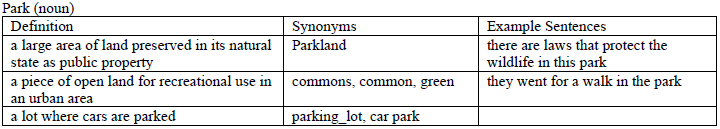
\includegraphics[width=5in]{figures/candidate-word-park-wordnet.png}
    \caption{Candidate word senses for the word \textit{park} from the WordNet database}
    \label{fig:candidate-word-park-wordnet}
\end{figure}

\subsection{Word sense disambiguation}

Using the information provided in WordNet, it is possible to perform word sense disambiguation. For a word in the schema and the metadata tags, we create a context using surrounding information available in the metadata. Similarly, we create a context for a word sense using the synonyms and the example sentences. After creating the contexts, we are able to compare the word with each candidate word sense using their contexts. If the two contexts are highly similar, then the metadata word is semantically enriched by attaching the definition of the word sense.

\begin{figure}
    \centering
    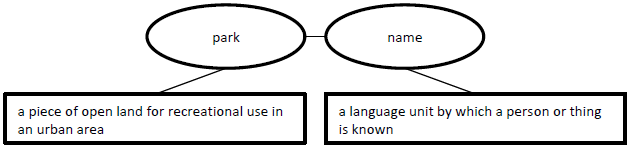
\includegraphics[width=5in]{figures/semantically-enriched-attribute.png}
    \caption{Semantically enriched attribute}
    \label{fig:semantically-enriched-attribute}
\end{figure}

While creating the contexts for the words and word senses, we do not add every word in the surrounding information to each context, since most of these words do not contribute to disambiguating word sense. For example, a sentence in the surrounding information can contain nouns, verbs, adjectives, prepositions, etc. We use part-of-speech tagging by the Hidden Markov Model to identify a word in a sentence as a noun, verb, etc. To simplify our work, we only add noun words to the context; we argue that nouns can contribute the most to word sense disambiguation. Each context therefore consists of a set of nouns. We then choose the word sense that has the most number of context word overlaps.

The overlapping of words between two contexts is also known as the gloss overlap. Gloss overlaps increases the chance of finding similarities between contexts, since related contexts tend to contain many common words. Finding the similarity by using gloss overlaps is known as the Lesk method~\cite{lesk1986automatic}. By using the Lesk method, we perform syntax-driven semantic analysis, where the context words are just items in a collection and we count how many items are overlapping.

Once we disambiguate the word, we attach the definition to the word. We name the step to attach definitions to words in metadata as \textit{semantic enrichment}. The words in the attributes of a schema and in the tags are semantically enriched. An example of a semantically enriched schema attribute, \textit{park name}, is shown in \autoref{fig:semantically-enriched-attribute}.

We provide an example of \textit{semantic enrichment} next. Using the metadata of \autoref{fig:example-parks}, we create the context of the word \textit{park} using \textit{table description}, \textit{category}, and \textit{tags}. Similarly, for each candidate word sense of \textit{park} in \autoref{fig:candidate-word-park-wordnet}, we use the \textit{definition}, the \textit{synonyms}, and \textit{example sentences} to create the context. After performing part-of-speech tagging for the \textit{table description}, the \textit{category}, and the \textit{tags}, we collect all the nouns into a list, which serves as the context for the tag word \textit{park}. Similarly, the nouns from the definition, the synonyms, and the example sentences are collected into a list, which serves as the context of each candidate word sense. The contexts for \textit{park} as well as all candidate word senses are shown in \autoref{fig:contexts-park-candidate}.

To compare between the tag word context and the word sense contexts, we find the number of overlapping items between each pair of sets. After stemming each word in each context, the number of overlapping items between \textit{park} and \textit{candidate word sense 1} is 1, for \textit{candidate word sense 2} it is 2, and for \textit{candidate word sense 3} it is 0. Therefore we select word sense \textit{candidate word sense 2}, to semantically enrich the tag word \textit{park} in \autoref{fig:example-parks}. Each semantically enriched tag is now called a \textit{topic}.

\begin{figure}
    \centering
    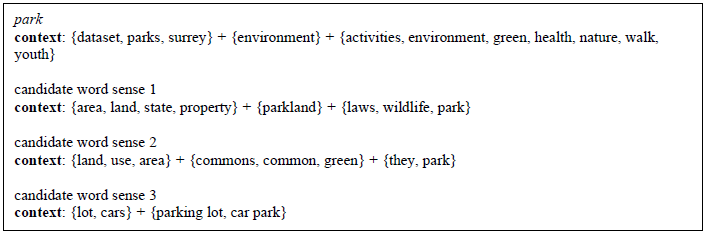
\includegraphics[width=5in]{figures/contexts-park-candidate.png}
    \caption{Contexts for tag \textit{park} and candidate word senses}
    \label{fig:contexts-park-candidate}
\end{figure}

Semantic enrichment of words can be viewed as a metadata generation problem, where we identify distinct concepts. When each concept consists of a group of words that have similar meanings, we are able to find all words belonging to the same concept instantaneously.

\subsection{Solution to semantic heterogeneity: dictionaries}
\label{ssec:SolutionToSemanticHeterogeneityDdictionaries}

When two elements (either tags, attributes, or other types of data) are highly similar in meaning, but are represented with different words or phrases, we rely on external resources such as a domain dictionary to determine if the two elements are similar. Using the domain dictionary, we are able to find all synonyms of a word. Even if two words are not synonyms of each other, they may still be semantically related.

Since a word can have many senses, the WordNet dictionary is a database that stores synonyms for each word sense. The set of synonyms with the same sense is called a \textit{Synset}. WordNet has a separate entry for each sense of a word (the example in \autoref{fig:candidate-word-park-wordnet} has three entries), and indicates which Synset the entry belongs in. It is then possible to compute the semantic distance between a pair of Synsets.

To quantify the distance between word senses, one approach is to let each word sense in the database be connected to its closely related senses by directed edges in a graph, representing semantic relations between them \cite{cruz2005role}. The types of relations include synonym, hypernym, hyponym, and antonym. Each type of relation has a specified weight, and each directed edge of the relation type is given the weight. The semantic distance between two word senses is computed by selecting the optimal path from all the candidate paths, after averaging the weights along each path.

For example, when we compare \textit{dog}(\textit{feline mammal usually having thick soft fur and no ability to roar: domestic cats; wildcats}) with \textit{cat}(\textit{a member of the genus Canis that has been domesticated by man since prehistoric times; occurs in many breeds}), the similarity between the pair of values determined by WordNet's \textit{path similarity} function is 0.2.

Another way to calculate the distance with WordNet is to use the information content of the lowest common subsumer \cite{Resnik1970Using}. All the senses of all words are organized into a tree hierarchy. For example, the words \textit{skating park} and \textit{amusement park} are daughters of \textit{park}, and if \textit{park} is the most immediate common ancestor between them, then \textit{park} is the lowest common subsumer. To calculate the distance between two words, one can estimate the probability of encountering the lowest common subsumer. For example, if there are a total of 100,000 occurrences of \textit{park} with the same sense, then this number is used to calculate a probability value which becomes the distance between the two words.

%%%%%%%%%%%%%%%%%%%%%%%%%%%%%%%%%%%%%%%%%%%%%%%%%%%%%%%%%%%%%%%%%%%%%%
\section{Schema matching}
\label{sec:SchemaMatching}

In this section, we give a detailed explanation of schema matching and its extensions \cite{Rahm2001Survey}. Schema matching is an algorithm that compares a pair schemata, where attributes in one schema are compared to attributes of the second schema to find a match. The match operator is widely used in many applications~\cite{Dong2012Proceedings,Rahm2001Survey,10.1145/3183713.3183729}, and it is a valuable tool for metadata management. Schema matching takes a pair of schemata as input (i.e.,~two sets of attributes to be matched), and identifies a set of pairs of attributes between the two schemata that are similar according to some criteria. Each in the matching is a triple in the form of (a, b, c), called a correspondence, where a is an attribute from the first schema, b is an attribute from the second schema, and c is a score for the pair of matched attributes according to some matching criteria.

More formally, let a correspondence be a triple:
\[
(A_{si},A_{s'j},c), \; \textrm{for} \; A_{si}\in A_{s} \; \textrm{and} \; A_{s'j}\in A_{s'},\text{and }s\neq s'
\]
where $c$ is the score in the range {[}0, 1{]}, and $c$ = 1 indicates a perfect correspondence between $A_{si}$ and $A_{s'j}$ . The comparison criterion between a pair of attributes could be equality, subsumption, overlap, etc.

We give a description of pairwise schema matching next. We first compare each attribute of the first schema to every attribute in the other schema. Based on a criterion (such as overlap of alphanumeric characters in the attribute names), we compute the similarity score between each pair of attributes. We then apply any matching constraints required to create correspondences between pairs of attributes. A user can choose to place different constraints, and these constraints are enforced during schema matching. One example of a constraint is that each correspondence must have a score above a threshold set by the user.

Another constraint frequently used in many existing schema matching algorithms is the one-to-one cardinality constraint on the correspondences, which ensures that once an attribute participates in a correspondence, it cannot participate in another correspondence. When such a constraint is enforced, the correspondence is a matching. A schema matching algorithm can use an existing algorithm for matching to enforce the one-to-one cardinality constraint. For example, it can resolve two or more pairs that conflict with each other by choosing the pair that is the most probable. Alternatively, all possible matchings can be enumerated, and the best matching is selected.

There are many possible ways to implement a schema matching algorithm. Typically, under the following assumptions, an algorithm can be implemented correctly:

\begin{itemize}
\item The cardinality constraint on correspondences between a pair of schemata is one-to-one. However, this constraint can be relaxed if needed.
\item A schema is present for each table, which allows schema matching to be performed instead of matching the header rows.
\item When a pair of attributes has a high score, it has a high similarity according to some matching criteria.
\end{itemize}

When the score computed is in the range of 0 to 1, we can model the score as the probability that the pair of attributes fulfills the specified criteria. Based on the probabilities, we can then rank all correspondences by their scores or compute other statistical measures.

We give an example using \autoref{fig:example-parks} and \autoref{fig:example-park-specimen-trees}. We let a pair of schemata be
\begin{quote}
    \textit{Parks}(\textit{park\_name}, \textit{location}, \textit{service\_classification}), and \\
    \textit{ParkSpecimenTrees}(\textit{location}, \textit{park}, \textit{tree\_species}).
\end{quote}

We perform matching between the two sets of attributes. We first compare \textit{Parks.park\_name} with \textit{ParkSpecimenTrees.location}, and then with \textit{ParkSpecimenTrees.park}, and so on. If we use the simple \textbf{\gls{matching criterion}}: find the proportion of overlapping characters, then the scores for the comparisons are 0.25, 0.67, and so on. If the one-to-one cardinality constraint is enforced, we must only choose one pair of attributes such that neither of the two attributes appears in other correspondences, and that the sum of the correspondence scores is maximized. In the example, the pairs of attributes chosen as the correspondences are
\begin{quote}
(\textit{Parks.park\_name}, \textit{ParkSpecimenTrees.park}, \textit{0.67}), \\
(\textit{Parks.location}, \textit{ParkSpecimenTrees.location}, \textit{1.0}), and \\
(\textit{Parks.service\_classification}, \textit{ParkSpecimenTrees.tree\_species}, \textit{0.32}).
\end{quote}
If the one-to-one cardinality constraint is relaxed, then the chosen correspondences are changed.

\subsection{Using schema matching on open data}
\label{ssec:UsingSchemaMatchingOnOpenData}

Schema matching does not necessarily have to operate only on attributes in schemata. We can use the algorithm to find a match between two sets of tags or between any pair of set-like data. The two sets can even be heterogeneous, where one set contains attributes and another set contains tags.

Therefore a correspondence can also be a triple:
\[
(L_{si},L_{s'j},c), \; \textrm{for} \; L_{si}\in L_{s} \; \textrm{and} \; L_{s'j}\in L_{s'}, \; \textrm{and} \; s\neq s'
\]
where $c$ is the score in the range [0, 1], and $c$ = 1 indicates a perfect correspondence between $L_{si}$ and $L_{s'j}$ . Schema matching between pairs of attributes and pairs of tags follow the one-to-one cardinality constraint.

We can use schema matching to compare other types of data such as long sentence descriptions and schema structure \cite{Sorrentino2011NORMS}. In \cite{10.1145/1066157.1066283,Duchateau2009YAM}, metadata such as schema version and namespaces were used in schema matching. It is also possible to perform schema matching using the data values in data instances \cite{Rahm2001Survey}. In our work, we use schema matching to find matching between a set of attributes and a set of tags, which we call the semantic labeling. Each pair of attribute and topic is called a semantic label.

Let a semantic label be a triple:
\[
(A_{si},L_{s'j},c), \; \textrm{for} \; A_{si}\in A_{s}\ \; \textrm{and} \; L_{s'j}\in L_{s}
\]
where $c$ is the score in the range {[}0, 1{]} and $c$ = 1 indicates a perfect labeling between $A_{si}$ and $L_{s'j}$.

The cardinality constraint on semantic labeling of attributes and topics is many-to-one (i.e., a topic can have many attributes). We did not enforce the one-to-one cardinality constraint, because the output matching is too restrictive. To implement schema matching between attributes and tags, we specifically consider three cases of the many-to-one cardinality constraint.

In the first case, an attribute may correspond to multiple tags. We disallow this case because when an attribute is labeled with too many tags, there will be too much computation in the subsequent step (within the table search algorithm) of the metadata augmentation algorithm. But when there are multiple tags that are synonyms of each other, an attribute should correspond to all of these tags. We deal with synonyms in the partitioning algorithm of metadata augmentation. In the second case, many attributes in one schema may correspond to one tag. We allow this case. When matching between attributes and tags, it is desirable to have a tag participating in multiple correspondences because we only have a limited number of tags. The third case is that a tag may correspond to many attributes, where each attribute is from a different schema. We allow this case because this cardinality constraint on correspondences will produce a mapping similar to the data integration scenario, where the mapping allows a uniform access to data in all data instances, which is similar to what we want to achieve as well. The many-to-many cardinality constraint cannot be enforced. As discussed in a data integration scenario, GLAV mappings are typically disallowed because there are too many possible candidates. Finding the optimal mapping is intractable \cite{Ehrig2004QOM}.

\subsection{Variations of schema matching}
\label{ssec:VariationsOfSchemaMatching}

The minimum form of schema matching does not usually produce correspondences accurately. Many variations of the minimum form are possible. Different variations of schema matching can improve the speed of matching as well as the quality of the correspondences. The matching criteria can be changed to reflect the similarity of attributes more accurately. One can use any linguistic-based criterion to compare the names of attributes, or use constraint-based criterion to compare the properties of the attributes. In constraint-based matching, an average can be computed for the value of a numeric column. Other statistical quantities can be computed with the goal of characterizing the data distribution of the column. The matching criterion compares two attributes based on their data distributions. In contrast, the work in \autoref{ssec:SupervisedLearningForSchemaLabeling} performed matching using constraint-based criteria.

In linguistic-based criteria, a dictionary or thesaurus can be used to find the semantic similarity. We explain our linguistic-based criteria using a dictionary. Suppose that the word sense (i.e., the definition) of each word in an attribute is known. Then, when attributes are compared, the definitions of the words are compared instead. If it is possible to find the semantic distance (a numeric quantity) between the word senses, then the semantic distance of the attributes can be computed. The attribute \textit{park name} with its attached definitions is shown in \autoref{fig:candidate-word-park-wordnet}.

We use the WordNet dictionary to retrieve the definition of words, and compute the semantic similarity between a pair of values using WordNet's built-in functions. The details have been explained in \autoref{ssec:SolutionToSemanticHeterogeneityDdictionaries}.

We can also compute the semantic similarity between two values using pre-trained word embedding vectors. Words in an attribute are encoded as word embedding vectors using FastText \cite{Mudgal2018Deep,Nargesian2018Table}, a variant of Word2Vec. A pair of vectors can be compared, and if two words are used under similar contexts, they should also have similar vectors. When comparing two sequences of words, the distance between their vectors is computed.

The minimum form of schema matching used a matching criterion that counts the proportion of overlapping characters of attribute names. A more sophisticated criterion at the character level is an N-gram distance function that computes the similarity between a pair of values \cite{loper-bird-2002-nltk}. Each value is transformed into a multiset of character n-grams. For example, we use the values \textit{`EastPark'} and \textit{`SouthPark'} to illustrate how to compute the similarity between them. The bigrams of \textit{`EastPark'} are [\textit{`Ea'}, \textit{`as'}, \textit{`st'}, \textit{`tP'}, \textit{`Pa'}, \textit{`ar'}, \textit{`rk'}], and the bigrams for \textit{`SouthPark'} are [\textit{`So'}, \textit{`ou'}, \textit{`ut'}, \textit{`th'}, \textit{`hP'}, \textit{`Pa'}, \textit{`ar'}, \textit{`rk'}]. The similarity is the proportion of shared n-grams between the two values, given by:

\[
\frac{2\times \left|ngrams(value1)\bigcap ngrams(value2)\right|}{\left|ngrams(value1)\right|+\left|ngrams(value2)\right|}
\]

Between \textit{`EastPark'} and \textit{`SouthPark'}, there are 3 shared bigrams [\textit{`Pa'}, \textit{`ar'}, \textit{`rk'}]. The similarity is therefore 6/15 = 0.4.

Another variation of schema matching is to perform matching at the instance level. Matching at the instance-level compares the data values in the data instances instead of only comparing the attributes. For tabular data instances, matching is done between the table values instead of the table headers, by comparing data values in table columns, with the goal of finding which data column pairs share the most values. Matching at the instance-level is known as \textit{entity matching}. The work in \cite{Mudgal2018Deep} used instance-level matching to determine whether or not a pair of attributes is in the same data domain. Works in \cite{Rahm2016Case} used natural language processing (NLP) and deep neural network (DNN) techniques to improve the ability to resolve values for entity matching. If precise matching is required, then each of the values needs to resolve to real-world entities (such as a concept in an ontology). This process called \textit{entity resolution}. In open data there is typically no real-world entity information provided \cite{books/sp/bellahsene11}, and therefore instance-level matching cannot be performed with precision. A course-grained instance-level matching approach uses document similarity measures (such as TF/IDF) \cite{Duchateau2009YAM}, by treating each column as a document (with values of a column aggregated into a single document). This approach performs poorly since individual values such as an address of a place requires more effort to identify, and therefore similarity between documents is typically low.

One can also perform matching with a combination of matching criteria within the same algorithm \cite{Sorrentino2011NORMS}. If an instance-level matching criterion is used in addition to a schema-level matching criterion, the instance-level criterion can add additional evidence for choosing the best correspondences. The reason is that each schema matching criterion specializes at evaluating certain types of data, because each criterion has a distinct similarity function. For example, a criterion that counts the proportion of word overlaps in attribute names is likely to produce different similarity values than a criterion that computes the semantic distance between words using a dictionary.

There are two ways to combine different matching criteria within the same algorithm, \textit{composite} and \textit{hybrid}. Composite matching combines the output attribute pairs from multiple independent matchings by merging the different sets into one set. For example, the set of pairs from one matching (with some criterion) is combined with the set from another matching (with another criterion) by removing conflicting pairs. Hybrid matching uses multiple matching criteria within the same matching algorithm. For each pair of attributes compared, a score is computed using multiple matching criteria, and the two scores are combined. A typical way to combine the scores is to compute a weighted average, where the weights are provided before matching \cite{DBLP:journals/debu/ChenGHTD18}. The weights can be trained by linear regression \cite{Ehrig2004QOM} such that the more effective criterion is given a greater weight. Other variations of hybrid matching exist. In \cite{Giunchiglia2005Semantic}, a decision tree is trained over a number of matching criteria, where the next matching criterion to use is decided based on the score produced by a previous score. In \cite{Moawed2018Arabian}, a neural network is trained that maps attribute features to Euclidean space. The vectors in Euclidean space are compared to compute the similarity scores.

%%%%%%%%%%%%%%%%%%%%%%%%%%%%%%%%%%%%%%%%%%%%%%%%%%%%%%%%%%%%%%%%%%%%%%
\section{Semantic labeling}
\label{sec:SemanticLabeling}

Once the cardinality constraint is enforced in the schema matching algorithm, semantic labeling can be performed. A semantic labeling is a mapping between an attribute and a tag (the header to a column), indicating that the data in the column contains data in the topic's domain. To create the semantic labeling for one schema, we perform schema matching between an attribute of the schema and every tag, similar to the approach discussed in \cite{Dong2012Proceedings,Salakhutdinov2009Semantic}. The attribute-tag pairs in the match are added to the result set; we call each attribute-tag pair a semantic label. An example of semantic labeling is shown in \autoref{fig:example-semantic-labeling}.

\begin{figure}
    \centering
    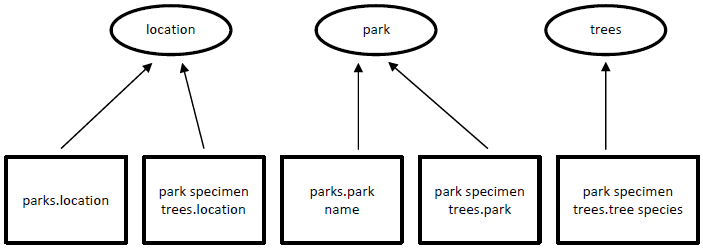
\includegraphics[width=5in]{figures/example-semantic-labeling.png}
    \caption{Example of a semantic labeling between attributes and tags.
    Each circle represents a tag, and each rectangle represents an attribute. There are two tables, \textit{parks} and \textit{park specimen trees}, each attribute of either table is mapped with a tag.}
    \label{fig:example-semantic-labeling}
\end{figure}

\subsection{Semantic labeling algorithm}
\label{ssec:SemanticLabelingAlgorithm}

For each text item $L_{sj}$ in the list of text items $L_{s}$ of data instance $s$, we add it to the set $L$. In our work, the text items are restricted to the tags. Then we perform schema matching between attributes $A_{s}$ and tags $L$; and according to the constraints defined in \autoref{ssec:UsingSchemaMatchingOnOpenData}, we create a semantic label $(A_{si},L_{s'j},c)$ for a pair of $A_{si}$ and $L_{s'j}$ with a high match score $c$. We use a threshold, and only add pairs with $c$ above the threshold that do not conflict with any existing constraints in schema matching. Since $s=s'$ or $s\neq s'$, there are $N$ or fewer semantic labels for $N$ attributes in a schema.

If there is a tag $L_{sk}$ in the existing metadata of the data instance that does not participate in any semantic labels, we create a label $(null,L_{sk})$ for it.

We give an example using \autoref{fig:example-parks} and \autoref{fig:example-drainage-catch-basins}. Let the input be the set of tags \{\textit{environment}, \textit{green}, \textit{nature}, \textit{parks}, \textit{trees}, \textit{devices}, \textit{infrastructure}\}, as well as a schema \textit{Parks}(\textit{park name}, \textit{location}, \textit{service classification}). The initialization step may generate the following semantic labels: (\textit{park name}, \textit{parks}), (\textit{location}, \textit{environment}), (\textit{service classification}, \textit{infrastructure}). In addition, let another schema be \textit{DrainageCatchBasins}(\textit{device type}, \textit{device size}), and the semantic labels be (\textit{device type}, \textit{device}), (\textit{device size}, \textit{infrastructure}).

Notice that both schemata have mappings to \textit{infrastructure}, but only one is suitable to contain this tag. The reason is because \textit{infrastructure} is used in different contexts in the two schemata. From the context of use, the word is more relevant to describe the structure built such as catch basins, rather than a service that may involve \textit{infrastructure}. In our main algorithm in \autoref{sec:IterativeApproach}, one of the two labels is not included in the result. We use the heuristic that \textit{DrainageCatchBasins} already contains the tag \textit{infrastructure} in its metadata, so it should keep the tag. In more complicated cases where neither table contained the tag originally, it is more difficult to decide.

%%%%%%%%%%%%%%%%%%%%%%%%%%%%%%%%%%%%%%%%%%%%%%%%%%%%%%%%%%%%%%%%%%%%%%
\section{Finding relatedness between tables}
\label{sec:FindingRelatednessBetweenTables}

Normally, tables are related by foreign key constraints, but in open data there are usually no foreign key constraints that relate tables together. Given one table, it is difficult to select related tables because there is no guidance from the foreign key constraints. We therefore discuss an algorithm that searches the tables to find how tables are related. We first show how table search in \cite{Nargesian2018Table} works. Given a table as the query, the goal is to find tables (top-k) that are unionable by searching all tables in a repository. The measure of unionability is defined by the number of attribute pairs between two tables that store similar kinds of data, and therefore it is possible to merge the rows of these tables together by aligning the unionable attributes. In contrast, the joinability measure is defined by the number of attribute pairs that have some values that are the same.

\subsection{Table search on open data}
\label{ssec:TableSearchOnOpenData}

The table search algorithm relies on the schema matching algorithm. The query table is compared with every other table in a pairwise manner. For each pair of tables, a column in the first table is compared with every column in the second table. For each pair of column comparisons, each value of the first column is compared with every value of the second column.

Three metrics are used to measure how similar two columns are: \textit{value overlap}, \textit{class overlap}, and \textit{natural language similarity}. The three metrics are three statistical tests to determine if a pair of columns are in the same data domain. The value overlap measure is based on the number of unique pairs of values that are the same between two columns. The class overlap additionally incorporates the semantic closeness of two values. It uses an ontology to find the distance between two values. When comparing two sets, a hypothesis test shows how likely the two sets, $A$ and $B$, are from the same domain $D$. The number of overlapping values, $t$, is calculated, and a cumulative distribution function is calculated over a hypergeometric distribution as follows:
\[
F(t|A,B) = \sum\limits _{0\le s\le t}\frac{C(n_{a},s)C(n_{D}-n_{a},n_{b}-s)}{C(n_{D},n_{b})}
\]
where $C(a, b)$ is a combination $a$ choose $b$. The natural language similarity first encodes each value into a fixed-dimension word embedding vector, which allows the comparison between two columns by the mean and variance of the vectors for the columns.

A similarity score for a pair of columns is computed from the three statistical tests performed. The score is called the \textit{attribute unionability}. After all pairs of columns are compared, all the attribute unionability scores are then used to perform schema matching. For the best match between the two sets of attributes, a \textit{table unionability} score between the two tables is computed. For the given query table, it is then possible to find all other tables similar to the query table based on the unionability scores of tables.

Let the open data repository contain the tables in \autoref{fig:example-park-specimen-trees} and \autoref{fig:example-park-screen-trees}, \textit{park specimen trees} and \textit{park screen trees}. We compare the fourth column of \textit{park specimen trees}, $A$, with the third column of \textit{park screen trees}, $B$. Let $A=$\{\textit{`rubrum'}, \textit{`rubrum'}, \textit{`nigra'}\} and $B=$\{\textit{`japonica'}, \textit{`rubrum'}, \textit{`nigra'}, \textit{`nigra'}\}. For the value overlap metric, the overlapping values are \{\textit{`rubrum'}, \textit{`nigra'}\}, thus $t=2$. Additionally, $n_D=|A+B|=7$, $n_A=|A|=3$, $n_B=|B|=4$. When $s=1$, the probability is computed by $C(4, 1) * C(4, 3) / C(7, 3)$. The cumulative function then sums up all probabilities of $s$ = 0 to $t$. However, due to both $A$ and $B$ being too large, computation of the probabilities requires hours, and requires further optimizations. The class overlap metric uses value similarities instead of value overlaps. The natural language similarity is computed using a vector representation for values. For example, when the vector dimension is 3, one such vector is [0.2, 0.4, 0.4]. Let the three metrics computed be \{$m_o$, $m_v$, $m_n$\}. The attribute unionability is computed by averaging the three metrics.

Let the attribute unionability scores for the pairs of columns be \\ \{(\textit{ParkSpecimenTrees.park name} and \textit{ParkScreenTrees.location} : 0.2), (\textit{ParkSpecimenTrees.park name} and \textit{ParkScreenTrees.species} : 0.7), \dots\}. After a best match is determined, let the table unionability be 0.4. When table search is performed with \textit{park specimen trees} as the query and the \textit{park screen trees} as a search candidate, they are unionable if 0.4 is above the decision threshold.

The authors relied on locality-sensitive hashing (LSH) to group all similar attributes from different tables into the same partition, which allows quick retrieval of all candidate tables containing an attribute similar to some given query attribute. However, building an LSH index takes a considerable amount of time, and depending on the problem, building such an index may not be desired.

\subsection{Modified table search}
\label{ssec:ModifiedTableSearch}

The table search algorithm discussed above does not assume any metadata other than the headers is available. We modify table search such that the tags will be utilized. Once semantic labeling is created for each table, we can perform table search by comparing pairs of semantic labels instead of comparing table columns. The attribute unionability score is omitted, and table unionability is defined as the number of overlapping tags (obtained from the semantic labels) between two tables. Table unionability is defined as $|L_{sq}\bigcap L_{s}|$. With one table $s_{q}$ as the query table, we find other tables $s\in D$ in the repository similar to the query table according to their table unionability scores. The tables $s\in D$ can then be ordered by their unionability scores.

Table search using semantic labeling is a crude way to find the relatedness of tables. Some tables may never be found while some irrelevant tables could appear to be related to the query. Even if the two tables do not share any common metadata tags, it is still possible that they are related. A semantic distance matching criterion can be used between tags instead of exact matches, since each tag is attached with its word definitions. Seemingly unrelated tables can then be related together by semantic similarity of their tags. Regarding the second question, additional tests can be performed once a table is found, to verify that it is indeed related.

%%%%%%%%%%%%%%%%%%%%%%%%%%%%%%%%%%%%%%%%%%%%%%%%%%%%%%%%%%%%%%%%%%%%%%
\section{Partitioning}
\label{sec:Partitioning}

Clustering is a common approach to group similar items together. In \cite{ilprints851}, a mediated schema is created by clustering the attributes, where similar attributes are grouped into one group, and a mediated attribute is created for each group along with its schema mappings. The work in \cite{Smith2011Unity} also performed clustering before a topic is assigned to each cluster. The input to clustering is a set of attribute-to-attribute correspondences, represented as a graph, where the attributes are nodes and the pairwise similarities are the edges with a score as the edge weight. They then performed hierarchical clustering on the graph to discover clusters of attributes. For each cluster, they assigned a topic to each cluster, and then labeled each attribute in the cluster with that topic.

When semantic labeling is created for the attributes, clustering is a good choice for the tags only or the attributes only in the semantic labeling. However, if we want to discover groups based on the attributes-to-topics semantic labeling (with attributes and tags together), it is less clear how to perform clustering.

\subsection{Partitioning semantic labels}
\label{ssec:PartitioningSemanticLabels}

An alternative to clustering is partitioning. We describe an algorithm that partitions a set of semantic labels. The input to the algorithm is the semantic labeling between the attributes and tags from one or more tables. A number of partitions are created initially, the set of semantic labels $(A_{si},L_{s'j})$ of one table $s$ is selected from the semantic labeling, and the tags $L_{s'j}$ in the semantic labels are used to create the initial partitions. Each partition is defined to be a tuple (\textit{Name}, \textit{Sem-Lab}, \textit{Attr-Set},\textit{Tag-Set}), where \textit{Name} is the name of the partition, \textit{Sem-Lab} is the set of semantic labels assigned to the partition, \textit{Attr-Set} is the set of attributes derived from the semantic labels, and \textit{Tag-Set} is the set of tags derived from the semantic labels. One partition is created for each tag in $L_{s'}$. The \textit{Name} for the partition is set to $L_{s'j}$, and the semantic label $(A_{si},L_{s'j})$ is added to the \textit{Sem-Lab} set. Similarly, we add the attribute $A_{si}$ and the tag $L_{s'j}$ to \textit{Attr-Set} and \textit{Tag-Set} respectively. We note that $s$ is the table where $A_{si}$ originates from, and $s'$ is the table the tag $L_{s'j}$ originates from.

For the remaining semantic labels in the input, we add each label to the existing partitions by the following rules: when the tag is similar to most of the tags in \textit{Tag-Set} in one partition, and the attribute is similar to most of the attributes in \textit{Attr-Set} of the same partition, we add the tag, the attribute, and the semantic label to the partition. The similarity is a binary value, where a score above the threshold $\varphi$ for a proportion higher than $\mu$ is considered similar. We may also need to decide whether to place a semantic label in an existing partition or to create a new partition, by the following rules: when either the attribute is not similar to any of the \textit{Attr-Set} or the tag is not similar to any of the \textit{Tag-Set} of existing partitions, but there exists a partition where for both the attribute and the tag, the similarity is above a lower threshold $\varphi '$ for a proportion higher than $\mu$, then we create a new partition using the semantic label.

To give an example, \textit{Parks} is the base table with semantic labeling \{(\textit{park name}, \textit{parks}), (\textit{location}, \textit{environment}), (\textit{service classification}, \textit{infrastructure})\}, we initialize partitions using the tags from these semantic labels. The partitions created are
\begin{quote}
(\textit{parks}, \{(\textit{Parks.park name}, \textit{parks})\}, \{\textit{Parks.park name}\}, \{\textit{parks}\}),
(\textit{environment}, \{(\textit{Parks.location}, \textit{environment})\}, \{\textit{Parks.location}\}, \{\textit{environment}\}), and
(\textit{infrastructure}, \{(\textit{Parks.service classification}, \textit{infrastructure})\}, \{\textit{Parks.service classification}\}, \{\textit{infrastructure}\}).
\end{quote}

Now consider the table \textit{ParkSpecimenTrees} with the semantic labeling \{(\textit{park}, \textit{park})\}. The semantic label (\textit{park}, \textit{park}) will be added to the partition named \textit{park}:
\begin{quote}
(\textit{parks}, \{(\textit{Parks.park name}, \textit{parks}), (\textit{ParkSpecimenTrees.park}, \textit{park})\}, \{\textit{Parks.park name}, \textit{ParkSpecimenTrees.park}\}, \{\textit{parks}, \textit{park}\})
\end{quote}

The partitioning algorithm may also take a set of unlabeled attributes as input. When there is no semantic label for an attribute, we cannot make tag comparisons, we can optionally compare with attributes in each partition only and add the attribute in the most similar existing partition. We also note that a semantic label can be added to multiple partitions if the similarity is high for all of these partitions, therefore the algorithm is not strictly performing partitioning.
\endinput

%    4. Solutions
%% The following is a directive for TeXShop to indicate the main file
%%!TEX root = diss.tex

\chapter{Solutions}
\label{ch:Solutions}

Having discussed the various fields of study related to augmentation of metadata in \autoref{ch:RelatedWork}: Related Work and a number of algorithms in \autoref{ch:Preliminaries}: Preliminaries, we now explain the algorithms for augmenting metadata. Each of the algorithms takes an input base table and a set of potentially related tables, and outputs a tuple $(\textit{Base-Table}, \textit{Tags-Set})$ as well as a set of tuples:
\[
(\textit{Table-Name}, \textit{Tags-Set})
\]
where $\textit{Table-Name}$ is the name of a table related to $\textit{Base-Table}$ and $\textit{Tags-Set}$ is the set of augmented tags for the table. The tags of each table in the set are normalized with respect to each other.


All four algorithms use the existing metadata to help augment additional tags, since we assumed that each table already contains some metadata describing the contents of the table. Two of the four algorithms serve as the baseline, one algorithm is our proposed algorithm, and the final algorithm is modified based on the proposed algorithm to improve performance. Each of the four algorithms compares data instances and augments metadata in different ways. In the next section, we discuss a common procedure shared by all four algorithms to achieve normalization of tags. We then explain each of the four algorithms in \autoref{sec:BruteForceApproach} to \autoref{sec:ImprovedIterativeApproach}.

%%%%%%%%%%%%%%%%%%%%%%%%%%%%%%%%%%%%%%%%%%%%%%%%%%%%%%%%%%%%%%%%%%%%%%
\section{Normalization of tags}
\label{sec:CommonProcedureForNormalizationOfTags}

\begin{figure}
    \centering
    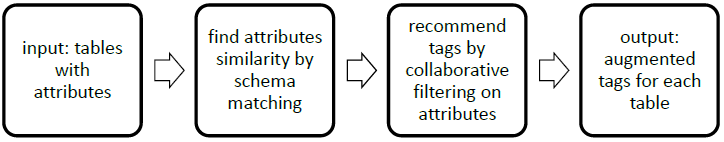
\includegraphics[width=5in]{figures/brute-force-algorithm.png}
    \caption{Brute Force algorithm for metadata tags augmentation}
    \label{fig:brute-force-algorithm}
\end{figure}

\begin{figure}
    \centering
    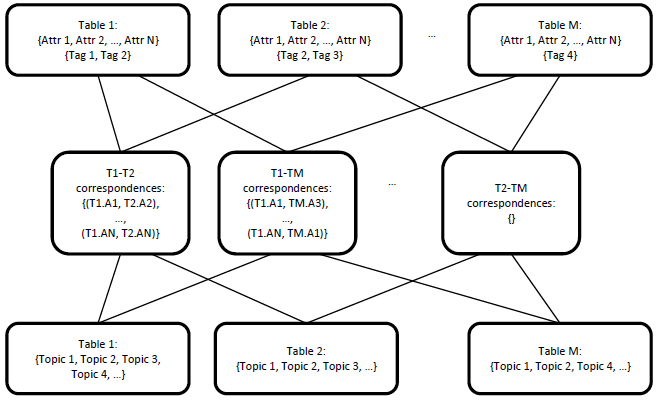
\includegraphics[width=5in]{figures/an-example-instance-brute-force.png}
    \caption{An example instance of tags augmentation by Brute Force}
    \label{fig:an-example-instance-brute-force}
\end{figure}

%\footnote{RAP: this paragraph is new; please check}
As introduced in Section~\ref{sec:intro:normalizing}, if there are two tags describing the same information, the user 
would likely want to add both tags to the metadata of all the tables containing this information. We seek all such tags, and ensure each table contains all the tags describing
the same information. We call this procedure \textit{normalization} of metadata tags. In
other words, a tag is added to all the relevant tables.

%\footnote{RAP: This paragraph has been rewritten. Please check} 
Consider the case there there are two tables, $TABLE_A$ and $TABLE_B$, that we know through some way (e.g., either through asking the users or through the methods described about schema matching) contain much of the information. Then, logically, we would want to see if we could augment the tags of $TABLE_A$ with some of the tags from $TABLE_B$. We call the tags of $TABLE_A$ and $TABLE_B$ $A$ and $B$ respectively. In other words we want to augment $A$ with some of the tags in $B-A$ and augment $B$ with some of the tags in $A-B$. Let the augmented sets of tags be called $A^{*}$ and $B^{*}$ respectively.

The overlap $A^{*}\cap B^{*}$ contains $A\cap B$; i.e., the number of tags that $TABLE_A$ and $TABLE_B$ have in common will increase.

Normalization produces the augmented sets $A^{*}$ and $B^{*}$ by comparing the sets $A$ and $B$ with each other, regardless of the algorithm used.


%\footnote{RAP: the rest of this subsection is very hard to follow, and I'm not sure that it adds to the reader's understanding. I suggest removing it.} The reason is that $A$ and $B$ are the only sources that the tags originate from. Suppose that there is a third set $C$ which contains all the tags in $A$ and $B$, then $A$ and $B$ do not need to compare to each other. The two sets can use the same criterion to compare to $C$ to obtain $A^{*}$and $B^{*}$. If $A$ and $B$ are initially empty, then the criterion can be created ahead of time, and the tags selected to each set will be normalized with respect to each other. However, if $A$ and $B$ are initially nonempty, then the criterion cannot be created without knowing the existing tags in $A$ and $B$, because the context of use for a tag may be different from the criterion\textquoteright s assumption.

%Using a real world example, let $A$=\ensuremath{\varnothing}, $B$=\ensuremath{\varnothing}, and $C$=\{\textit{park}, \textit{parkland}\}. The table of $A$ is created by one author, while the table of $B$ is created by another. Both tables contain data about \textit{parks} in a city. The two authors then agree that the two tables contain similar data, and therefore both $A$ and $B$ should contain \{park, parkland\}, without the need to examine $A$ and $B$ first. On the other hand, if $A$=\{\textit{park}\}, $B$=\{\textit{parkland}\}, and $C$=\{\textit{park}, \textit{parkland}\}, then the two authors need to examine $A$ and $B$ in order to reach a consensus. The consensus is that both the tags park, parkland are able to describe both tables, which becomes the criterion for adding the tags to another table $D$ containing data about \textit{parks} in a city as well. This example can be generalized to $n$ tables with tags $A_1, A_2, \dots A_n$. 

%We note that this procedure for comparing tables and tags is required for all algorithms that assumes each table\textquoteright s tags set is nonempty.

%%%%%%%%%%%%%%%%%%%%%%%%%%%%%%%%%%%%%%%%%%%%%%%%%%%%%%%%%%%%%%%%%%%%%%
\section{Brute force approach}
\label{sec:BruteForceApproach}

We first explain an algorithm we call Brute Force, as shown in \autoref{fig:brute-force-algorithm}, which serves as a baseline algorithm. \autoref{fig:an-example-instance-brute-force} is an example instance of tags augmentation by Brute Force. The algorithm is adapted from \cite{Smith2011Unity}, which we briefly explained in \autoref{ssec:ClusteringToReduceComplexity}. The algorithm consists of two separate steps, schema matching and collaborative filtering. Schema matching takes as input two sets of attributes for each pair of tables, and finds a set of correspondences between them. We enforce the one-to-one cardinality constraint between every pair of schemata. Collaborative filtering is then performed to recommend additional tags for each table. We adapted collaborative filtering from \cite{conf/esws/EllefiBDT16}, which was explained in \autoref{ssec:RecommendationOfSimilarDataUsingDataLinking}. For each table $A$, based on the similarity of its attributes with another table(s) $B$, the tags from $B$ are added to $A$'s tags set. If $A$ and $B$ share many similar attributes as determined by attribute correspondences, their tags sets should also be similar. The rule is parameterized by $k$ and $i$: when $A$ and $B$ share $k$ similar attributes, then they should share the subset $i$ of tags. We made a simplification of collaborative filtering by restricting $B$ to be a single table only.

We use \autoref{fig:example-parks} and \autoref{fig:example-park-specimen-trees} as an example. Let $A$ be \textit{Park} and let $B$ be \textit{ParkSpecimenTrees}. Suppose that the tags set of \textit{Park} is \{\textit{parks}\} and the tags set of \textit{ParkSpecimenTrees} is \{\textit{trees}\}. Comparing between \textit{Park.park\_name} and \textit{ParkSpecimenTrees.park} using the N-gram matching criterion yields a similarity score of 0.39. If the threshold is 0.3 and there are no other cardinality constraints, then this pair of attributes forms a correspondence (\textit{Park.park\_name}, \textit{ParkSpecimenTrees.park}, \textit{0.39}). If we suppose that $k$=1 and the subset $i$ is all tags in the tables, then the augmented set of tags for both tables is \{\textit{parks}, \textit{trees}\}.

Given a set of attribute correspondences in \cite{Smith2011Unity}, clustering is then performed to find groups of similar attributes, and each group is labeled with a tag. By performing clustering, a \textit{holistic view} of attribute groups can be obtained. Most existing schema matching algorithms only work well when matching a smaller number of schemata in the repository without obtaining a holistic view. In \cite{10.1145/2396761.2398468}, they used a statistical approach to find a unified model that generates matchings given a number of input schemata. Although a holistic view can be obtained, scalability issues arise due to the need to enumerate all possible models when there are too many schemata in a repository.

A holistic schema matching algorithm is proposed in \cite{Rahm2016Case}, where they first performed pairwise matching between all pairs of schemata, and then clustered the correspondences. The conclusion from a holistic view is that all attributes in the same cluster are highly similar according to some matching criteria. Note that the algorithm does not take into account a base table, which suggests that the output is not optimized for the base table. We replaced clustering with collaborative filtering. When $A$ is the base table, it will be compared with every other table so that tags from any of these tables can be added to $A$'s set. Although there may be too many tags added to the base tables set, we argue that increasing recall while sacrificing precision is a reasonable tradeoff. Normalization of tags can be achieved by assuming each table's tags set is nonempty.

\subsection{The issue with the number of comparisons}

The Brute Force algorithm has the issue of high computational cost due to schema matching performed on all table pairs. For a large number of tables, the number of pairwise attribute comparisons grows exponentially relative to the number of tables and the number of attributes in each table. For example, for $M$ tables and $N$ attributes, the number of comparisons is $C(M,2)\cdot(N\cdot N)$. When there are 100 tables, each with 3 attributes, then there are 44,550 comparisons.

%%%%%%%%%%%%%%%%%%%%%%%%%%%%%%%%%%%%%%%%%%%%%%%%%%%%%%%%%%%%%%%%%%%%%%
\section{Data driven approach}
\label{sec:DataDrivenApproach}

We describe our second baseline algorithm, modified based on \cite{10.1145/3184558.3191601} and briefly explained in \autoref{ssec:SupervisedLearningForSchemaLabeling}. We call the algorithm `Data Driven'. A multiclass classifier is learned from data. Using the classifier, each attribute of a table is assigned a tag (i.e., a class) from a known vocabulary. At the end of Data Driven, the tags assigned to attributes of a table become the augmented tags. We provide as many tables as there are in the repository to the classifier, so that the tags set of every table in the repository is augmented.

The classifier uses a number of matching criterion to compute the similarity score between an attribute and a candidate tag. The hybrid score is computed by combining the scores of each criterion, as discussed in \autoref{ssec:VariationsOfSchemaMatching}. For the pair of attribute and tag with the highest weighted score, the tag becomes the class for the attribute. To train the classifier, we train a weight for each combination of a matching criterion and a tag. The weights are represented as a matrix W, where each row are weights for single tag and each column are weights for a single matching criterion. The supervised learning takes as input a set of pairs of attribute and tag, defined as:
\[
(A_{si}, L_{sj})\text{ for }A_{si}\in A_{s}, L_{sj}\in L_{s}, s\in D'
\]
where the attributes $A_s$ and tags $L_s$ originate from a table $s$ in a set ${D'}$. The set of all tags in the training data is $L$.

For every attribute $A_{si}$ , we create a similarity matrix for pairwise comparisons between the attribute and a tag $L_j$ using matching criterion $M_t$. The similarity matrix is multiplied with the matrix of weights, and the weighted similarity score is compared with the true label in the training data. The losses are used to adjust the weight of a matching criterion relative to other matching criteria. For each example $A_{sj}$ and for each class $L_i$ , the following is the loss: 
\[
\sum_{j}(l(L_{i},A_{sj})-\sum_{t}s(L_{i}|A_{sj},M_{t})\ast W_{M_{t}}^{L_{i}})^{2}
\]
where $l(L_{i},A_{sj})$ is the true label. It is 1 when $L_{i}$ is the class for $A_{sj}$ and 0 otherwise. $s(L_{i}|A_{sj},M_{t})$ is the similarity score the matching criterion $M_{t}$ produces, and $W_{M_{t}}^{L_{i}}$ is the weight for class $L_{i}$ and matching criterion $M_{t}$. The weight of each classifier is adjusted for each training pair $(A_{sj}, L_{i})$ once the accuracy of each matching criterion is computed in the loss function. A weight for a class $L_{i}$ for the $M_{t}$ matching criterion indicates the strength of $M_{t}$ at correctly predicting an attribute $A_{sj}$ to be in the class $L_{i}$.

Note that a limitation of Data Driven is that each attribute is assigned with a single tag only, so the maximum number of new tags augmented is the number of attributes of the table. In addition, the normalization assumes each table's tags set is empty. Our implementation is modified based on the FlexMatcher package provided by the BigGorilla project \cite{DBLP:journals/debu/ChenGHTD18}.

\subsection{Example of multiclass classification}

To show how to augment the tags set of a table using multiclass classification, let the test data be the \textit{Parks} table in \autoref{fig:example-parks}. Let \{\textit{parks}, \textit{environment}, \textit{nature}, \textit{green}, \textit{trees}, \textit{devices}, \textit{infrastructure}\} be the complete set of tags $L$. Let the matching criteria, $M$, be \{\textit{N-gram}, \textit{WordNet}, \textit{FastText}\} for hybrid matching.

Let the trained weights, $W$, of the matching criteria be:

\begin{table}[h!]
    \begin{center}
      \begin{tabular}{|l|l|l|l|l|l|l|l|}
        \hline
        & \text{N-gram} & \text{WordNet} & \text{FastText}\\
        \hline
        \textit{parks} & 0.3 & 0.4 & 0.3 \\
        \hline
        \textit{environment} & 0.2 & 0.35 & 0.45 \\
        \hline
        \textit{\dots} &  &  &  \\
        \hline
        \textit{infrastructure} & 0.7 & 0.2 & 0.1 \\
        \hline
      \end{tabular}
    \end{center}
\end{table}

Hybrid matching uses each criterion to compute the similarity score between an attribute and each of the candidate tags. For the attribute \textit{park name} in \textit{Parks}, let the similarity matrix be:

\begin{table}[h!]
\centering
    \begin{center}
      \begin{tabular}{|l|l|l|l|l|l|l|l|}
        \hline
        & \textit{parks} & \textit{environment} & \textit{nature} & \textit{green} & \textit{trees} & \textit{devices} & \textit{infrastructure}\\
        \hline
        \text{N-gram} & 0.6 & 0.2 & 0.3 & 0.3 & 0.2 & 0.5 & 0.3 \\
        \hline
        \text{WordNet} & 0.8 & 0.6 & 0.6 & 0.6 & 0.5 & 0.2 & 0.2 \\
        \hline
        \text{FastText} & 0.8 & 0.8 & 0.7 & 0.7 & 0.7 & 0.2 & 0.3 \\
        \hline
      \end{tabular}
    \end{center}
\end{table}

For example, the similarity of (\textit{park name}, \textit{parks}) is 0.6 with N-gram, 0.8 with WordNet, and 0.8 with FastText. Then the combined score is 0.6*0.3 + 0.8*0.4 + 0.8*0.3 = 0.74. In the same way, the combined scores for other candidate tags are (\textit{park name}, \textit{environment}, \textit{0.61}), (\textit{park}, \textit{green}, \textit{0.6}), and so on. If (\textit{park name}, \textit{parks}) has the highest score of 0.74, then the attribute \textit{park name} is assigned to \textit{park}. At the end of Data Driven, the \textit{Parks} table is augmented with \textit{parks} in its tags set.

%%%%%%%%%%%%%%%%%%%%%%%%%%%%%%%%%%%%%%%%%%%%%%%%%%%%%%%%%%%%%%%%%%%%%%
\section{Iterative approach}
\label{sec:IterativeApproach}

We now explain an algorithm that iteratively augments metadata tags given a base table, as shown in \autoref{fig:the-steps-iterative-approach}. The output is a set of tables related to the base table, where the base table and each of the related tables contains a normalized tags set. The iterative approach uses the existing small number of tags in tables in the repository, and augments a subset of tables in the repository with additional tags to make their metadata more complete. The subset of tables is related to the base table, which is consistent with the scope of augmenting metadata discussed in \autoref{sec:ScopeOfImprovingMetadata}. That is, since it is unnecessary for a user to look at all tables in the repository, only the tags set of the related tables are augmented. The algorithm emphasizes the process of normalization, such that tables containing overlapping information (i.e., in the data domain of some tag) have one or more shared tags.

The algorithm begins with an initialization step, which creates the semantic labeling (discussed in \autoref{sec:SemanticLabeling}) between attributes and tags for all tables in the repository. The initialization step facilitates normalization of the tags. We then apply an iterative method that integrates a table search step (discussed in \autoref{sec:FindingRelatednessBetweenTables}) and a partitioning step (discussed in \autoref{sec:Partitioning}). The table search step helps discover tables related to the base table. Between the base table and a related table, the partitioning step is performed on the set of semantic labels of the related table. Schema matching is performed throughout the algorithm to verify that a pair of items (either attribute or tag) correspond to each other. The iterative method will be explained in \autoref{ssec:IterativeMethod}. Finally, the tags in the partitions are added to each table's metadata, as explained in \autoref{ssec:FromPartitionsToMetadataTags}.

\begin{figure}
    \centering
    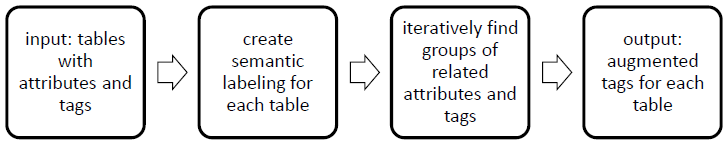
\includegraphics[width=5in]{figures/the-steps-iterative-approach.png}
    \caption{The steps in the iterative approach to augment metadata tags for tables}
    \label{fig:the-steps-iterative-approach}
\end{figure}

\subsection{Semantic labeling as the initialization step}
\label{ssec:SemanticLabelingAsTheInitializationStep}

The iterative method in our algorithm relies on an initialization step, which is performed before the iterative method. The initialization step takes as input a set of attributes and tags $(A_{s}, L_{s})$ for each table $s$ in the repository, and a semantic labeling between attributes and tags is found by schema matching (probabilistically as described in \autoref{ssec:UsingSchemaMatchingOnOpenData}). We then take the semantic labels as input, and for the base table, $s_q$, we create empty partitions using the tags in the semantic labels of $s_q$. We create a partition for each topic $L_{j}$ in $s_q$. For each semantic label, $(A_{si}, L_{j})$, we place the attribute $A_{si}$ and the tag $L_{j}$ to the sets in the partition of $L_{j}$ as explained in \autoref{ssec:PartitioningSemanticLabels}. We let the set of partitions of table $s_q$ be $S$. $S$ is then compared with the semantic labeling of the other tables in the repository, in the \textit{table search} step and the \textit{partitioning} step of the iterative method.

With the initialization step, we are able to modify the procedure for comparing two sets for normalization explained in \autoref{sec:CommonProcedureForNormalizationOfTags}. When comparing each pair of sets of tags, the sets have already been  partially normalized. During a preprocessing step, all known tags are collected from the metadata of each table. The set of all tags, $L$, is the vocabulary for all semantic labels and the candidate tags used for augmentation. We assume that the tags already created within a table may be incomplete, but together with tags from all tables, they are sufficient to describe the repository well. When the semantic labeling is performed, we compare a schema attribute with all possible tags instead of just the tags in its own metadata. The semantic labels created have received new tags from other tables, and therefore part of the normalization process has been performed already before the iterative method. The real world analogy is that humans tend to communicate with each other after they are certain what topics will be in the conversation, so that stochasticity in the outcome is reduced.

By performing semantic labeling in the initialization step, we improve the quality of the augmented metadata and the efficiency. The semantic labeling enhances the quality of the related tables retrieved by the table search step, due to the increased tag overlaps between tables. The semantic labels also increase the chance for the partitioning step to correctly place attributes and tags in the correct partition. Another benefit of the initialization step is to facilitate the improvement of the asymptotic computation cost by reducing the pairwise comparisons from exponential (i.e., between all pairs of attributes in Brute Force) to polynomial (i.e., between the tags in an iterative manner), since each table contains more tags for tag comparisons.

\subsection{Iterative method}
\label{ssec:IterativeMethod}

\begin{figure}
  \centering
  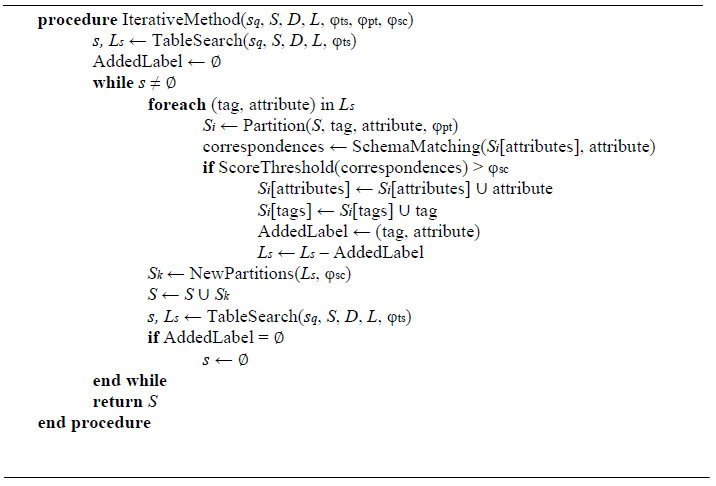
\includegraphics[width=5in]{figures/iterative-method.png}
  \caption{Iterative method}
  \label{fig:iterative-method}
\end{figure}

As proposed by \cite{Smith2011Unity}, to achieve normalization we need to find relationships between the metadata of all tables, and generate additional metadata that captures the relationships to make data more searchable and understandable.

Once we have performed table search and table recommendation, a group of tables is found to be related to a base table, thereby organizing the metadata of the existing tables, and finding relatedness.

Therefore, we need methods to organize the metadata and discover the relatedness.

Our main algorithm uses the table search outlined in \cite{Mudgal2018Deep} to approximate tables that are relevant to the base table.

We emphasize that augmenting metadata is only possible when a group of related tables can be found. A user who manually searches for related tables would encounter the same challenge.

Finding the interesting tags can be achieved by table searching, adopted from \cite{Nargesian2018Table} and \cite{conf/esws/EllefiBDT16}, which we explained in detail in \autoref{ssec:TableSearchOnOpenData} and \autoref{ssec:ModifiedTableSearch}.

Partitioning was explained in \autoref{ssec:PartitioningSemanticLabels}. We explained how we normalize the tags using the semantic labeling, briefly in \autoref{sec:SemanticLabeling}, and more in detail in \autoref{sec:IterativeApproach}. We can iteratively augment metadata of the base table and the tables we retrieved.

After we retrieve one candidate table, we perform schema matching again between the base table and the candidate table in order to augment metadata tags. We use the matched topic pairs from table search to obtain candidate attribute pairs, and then perform attribute-to-attribute schema matching to verify that each pair of attributes belongs to the same domain. For example, given that the overlapping tag is \textit{parks}, with semantic labeling of (\textit{parks}, \textit{Parks.park\_name}) and (\textit{parks}, \textit{Park\-Specimen\-Trees.park}), we know that the pair of attributes (\textit{Parks.park\_name}, \textit{Park\-Specimen\-Trees.park}) should be compared to verify that they are similar. Once the correspondence between the pair of attributes is confirmed, we can confirm that the tag \textit{parks} is a correct tag for both tables.

The \textit{iterative method} in \autoref{fig:iterative-method} takes $s_q$, $S$, $D$, $L$, $\ensuremath{\varphi}_{ts}$, $\ensuremath{\varphi}_{pt}$, $\ensuremath{\varphi}_{sc}$ as input, where $D$ is the set of all data instances in the repository, $L$ is the set of text items describing the data instances, $\ensuremath{\varphi}_{ts}$ is a threshold used for schema matching during the table search step, $\ensuremath{\varphi}_{pt}$ is a threshold used for schema matching during the partitioning step, and $\ensuremath{\varphi}_{sc}$ is a threshold used for schema matching during the verification step after items are placed in partitions.

Function \textit{TableSearch} is described in words in \autoref{ssec:ModifiedTableSearch}. We first select a table $s\in D$ that is most closely related to the current state $S$ of $s_q$. The relatedness is determined by the number of overlapping tags between the selected table $s$ and $s_q$. Next, for each semantic label in the selected table, use \textit{Partition} (described in \autoref{ssec:PartitioningSemanticLabels}) to compare the tag to each partition of $s_q$. Using \textit{Partition}, if the tag is similar to the tags in a partition, then use \textit{SchemaMatching} (described in \autoref{ssec:UsingSchemaMatchingOnOpenData}) to perform schema matching between the tag's mapped attribute and existing attributes in the partition. From \textit{ScoreThreshold}, if correspondences above $\ensuremath{\varphi}_{pt}$ can be created from the result of schema matching, add the tag and the attribute to that partition. If the tag is not highly similar to any tags in any partitions, but the tag is somewhat similar to tags in $s_q$ above a threshold score, then use \textit{NewPartitions} (described in \autoref{ssec:PartitioningSemanticLabels}) to create a new partition for the tag. Update the current state $S$ to include new partitions and tags. In the selected table $s$, remove tags that were added from its metadata, so that these tags will not overlap with the base table again in the next iteration. Repeat all of the above in a new iteration if it is still possible to find a table $s\in D$ related to the current state $S$ of $s_q$. The only matching criterion we used throughout the algorithm is N-gram.

\subsection{Iterative method example}
\label{ssec:IterativeMethodExample}

We use \autoref{fig:example-parks}, \autoref{fig:example-park-specimen-trees}, etc.~as an example. Let the base table be \textit{ParkSpecimenTrees} with the semantic labeling (\textit{location}, \textit{environment}) and (\textit{tree species}, \textit{trees}), (\textit{park}, \textit{parks}). Let the repository $D$ contain tables \textit{Parks}, \textit{GreenInfrastructureNetwork}, and \textit{DrainageCatchBasins}. We use the semantic labeling in \textit{ParkSpecimenTrees} to search other tables containing the maximum number of overlapping tags. The first table found is \textit{Parks}, with overlapping tags [\textit{environment}, \textit{parks}]. For every tag in \textit{Parks}, we find a partition that it belongs to. Let there be a semantic label (\textit{park\_name}, \textit{parks}) for \textit{Parks}. We compare it with the partition containing the tag \textit{parks}, which also contains \textit{ParkSpecimenTrees.park} in the set of attributes. We then compare the attribute \textit{park} in \textit{ParkSpecimenTrees} with \textit{park\_name} in \textit{Parks}, and find that the two attributes are similar. We add (\textit{park\_name}, \textit{parks}) to the partition, and remove the tag \textit{parks} from the list of tags of \textit{Parks}, so that \textit{parks} will not be an overlapping tag with the base table again in future iterations. After the first iteration, the base table contains tags [\textit{trees}, \textit{parks}, \textit{environment}, \textit{green}, \textit{nature}]. In the second iteration, let the table found be \textit{GreenInfrastructureNetwork} with tags [\textit{ecosystem}, \textit{sustainability}, \textit{green}] and semantic labels \{(\textit{ecological value}, \textit{ecosystem}), (\textit{hub or site}, \textit{green})\}. The base table overlaps with the tag green. By comparing the tags of \textit{GreenInfrastructureNetwork} with partitions in the base table, we find additionally that \textit{ecosystem} is similar to \textit{environment}, and \textit{sustainability} is similar to \textit{environment}. We perform schema matching between attributes of \textit{GreenInfrastructureNetwork} and attributes in the partition of \textit{environment}. Suppose that the correspondence score is above threshold $\ensuremath{\varphi}_{sc}$ for \textit{ecosystem}, and below threshold $\ensuremath{\varphi}_{sc}$ but above 0.5$\ensuremath{\varphi}_{sc}$ for \textit{sustainability}. We add \textit{ecosystem} to the partition containing \textit{environment}. We then create a new partition for \textit{sustainability} by \textit{NewPartitions}. Since there is no semantic label for \textit{sustainability}, the attributes set for the new partition is empty. Once the second iteration completes, the partitions of the base table contain the tags [\textit{trees}, \textit{parks}, \textit{environment}, \textit{green}, \textit{nature}, \textit{ecosystem}, \textit{sustainability}]. These tags are used to find tag overlaps with other tables in the repository, but \textit{Parks} and \textit{GreenInfrastructureNetwork} will not overlap in these tags. In the third iteration, we were unable to find any similar tables and we terminate the iterative method, as shown in \autoref{fig:partitions-park-specimen-trees}.

We provide a second example with \textit{Parks} as the base table. We find that our base table is similar to \textit{DrainageCatchBasins}, the overlapping tag is \textit{infrastructure}, where the semantic labels are (service \textit{classification}, \textit{infrastructure}) for \textit{Parks} and (\textit{device size}, \textit{infrastructure}) for \textit{DrainageCatchBasins}. After comparing the attributes with \textit{SchemaMatching}, we find that \textit{service classification} and \textit{device size} are not similar, nor is the attribute \textit{device size} similar to any other partitions. Thus we do not add (\textit{device size}, \textit{infrastructure}) to the base table partitions.

\subsection{From partitions to metadata tags}
\label{ssec:FromPartitionsToMetadataTags}

Each partition is a collection containing a set of attributes, a set of tags, and the mapping between attributes and tags. The iterative method takes a set of semantic labeling as input, and outputs the partitions of the base table. We show how to create a modified set of semantic labeling for each table found in \textit{TableSearch}, and how to augment tags of a table using semantic labeling. We let $A(a)$ and $B(b)$ be two tables where $a$ and $b$ are attributes, and let $A$ be the base table. Let tags of $A$ be $[X]$, and tags of $B$ be $[Y]$. Let semantic labeling of $A$ be ${(a, X)}$ and semantic labeling of $B$ be ${(b, Y)}$. Suppose that $X$ and $Y$ are similar, and $a$ and $b$ are similar. Thus there is one partition where the attributes are ${a, b}$ and the tags are ${X, Y}$. We also keep track of the mappings between attributes and tags as well as which table an attribute originates from. For each table, we collect all tags in all partitions where its attributes are assigned, and augment the table tags with any additional tags it does not already contain. For every attribute in a partition, we create a new semantic label for every attribute-tag pair. For example, in addition to the existing semantic labels, the semantic labels $(a, Y)$ and $(b, X)$ are created. Then table $A$ would collect both $X$ and $Y$ as the augmented metadata, and likewise for table $B$.

At the end of the third iteration in the example from \autoref{ssec:IterativeMethodExample}, the augmented tags for \textit{ParkSpecimenTrees} are [\textit{environment}, \textit{ecosystem}, \textit{trees}, \textit{green}, \textit{parks}, \textit{sustainability}], the augmented tags for \textit{Park} are [\textit{environment}, \textit{ecosystem}, \textit{parks}], and the augmented tags for \textit{GreenInfrastructureNetwork} are [\textit{environment}, \textit{ecosystem}, \textit{trees}, \textit{green}].

\begin{figure}
    \centering
    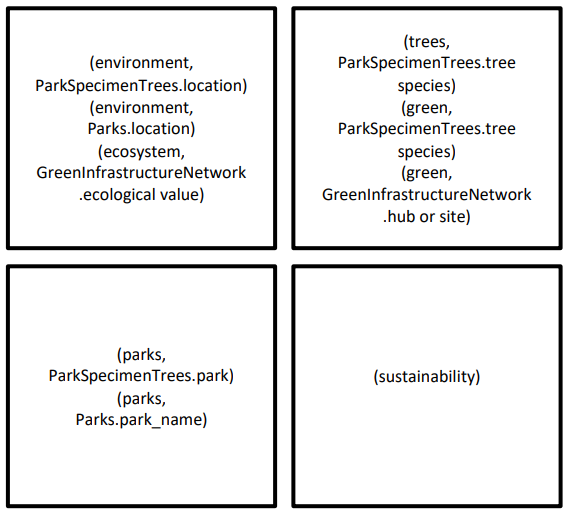
\includegraphics[width=5in]{figures/partitions-park-specimen-trees.png}
    \caption{Partitions of base table \textit{ParkSpecimenTrees} after the third iteration of the example in \autoref{ssec:IterativeMethodExample}. Each partition contains a set of attributes and a set of tags, as well as the mappings between them. They are represented as the set of semantic labels above.}
    \label{fig:partitions-park-specimen-trees}
\end{figure}

%%%%%%%%%%%%%%%%%%%%%%%%%%%%%%%%%%%%%%%%%%%%%%%%%%%%%%%%%%%%%%%%%%%%%%
\section{Improved iterative approach}
\label{sec:ImprovedIterativeApproach}

To perform semantic enrichment, we take the existing table metadata as input, and then create a common representation of information in the form of a list of tags.
With distinct concepts, it is easier to find metadata overlaps.
However, finding distinct concepts requires creating contexts for word sense disambiguation.
Recall that the term \textit{topic} is used for tag with a known dictionary definition, and it defines a data domain.
We rely on the semantics of words in the metadata to determine relatedness between data instances.

When metadata are semantically enriched, it is much easier to compare between the metadata and to semantically label attributes with tags. Next, we explain how schema matching uses semantically enriched metadata to effectively label attributes with tags, thus assigning additional context to attributes of a schema.

%We first talk about semantic enrichment and semantic labelling to resolve semantic heterogeneity.

%We first perform semantic enrichment for both attributes and tags, and create semantic labeling between attributes and tags.

The first step is to apply external knowledge such as a domain dictionary to determine the semantics, performed along with word sense disambiguation.
This step performs word sense disambiguation using metadata, and semantically enrich each attribute or tag by associating it with a WordNet Synset.
Since each word used in a tag can have more than one meaning, we attach a dictionary definition to each word in a tag as shown in \autoref{fig:semantically-enriched-attribute}, where we used metadata to disambiguate the words.

Once we disambiguate a word, we are able to identify other words with similar interpretations across all metadata of all tables.

Let us make two changes to Iterative. We name our new algorithm Improved Iterative. The first change is to perform semantic enrichment before semantic labeling during the initialization step. We apply semantic enrichment from \autoref{sec:SemanticLabeling}, where word sense disambiguation is performed on attributes and tags. The second change is to include more matching criteria for schema matching. We use hybrid matching from \autoref{ssec:VariationsOfSchemaMatching} to combine the similarity scores of the different matching criteria.

Enriching metadata relies on the availability of external knowledge, which we can use to assist in resolving conflicting word senses. We create contexts for attributes and tags. We use WordNet as our external knowledge base and the Lesk method discussed in \autoref{sec:SemanticLabeling} to semantically enrich the attributes and tags, and attach the semantics to the attributes and tags. The way that we enrich the attributes and tags is by finding the correct Synset of a word, where the semantics is given. The justification for performing semantic enrichment is that the open data metadata tags and attributes exhibit semantic heterogeneity, and we need to resolve the heterogeneity to allow pairwise comparisons to be effective. If attributes and tags are placed in the same partition, then they must overlap in the data domain, and the attribute names and tag names could be synonyms of each other.

Once semantics is provided by semantic enrichment, we perform schema matching using a matching criterion that assesses the semantic similarity. We chose N-gram as our only matching criterion in Iterative, which we do not think is effective for open data. Improved Iterative combines three matching criteria during schema matching: \textit{N-gram}, \textit{WordNet}, and \textit{FastText}. The weights used to combine the matching criteria are trained by hybrid matching.

\subsection{Initialization step}

As the first step before we perform the initialization step, we perform semantic enrichment (discussed in \autoref{sec:SemanticLabeling}) of attributes and tags for each data instance. For every word $w$ in each attribute $A_{si}$ or tag $L_j$, we perform word sense disambiguation by using gloss overlap between the context of a word sense $C(w)_k$ and the context of the word in the attribute $C(A_{si})_w$ or tag $C(L_j)_w$. The context of a word sense $C(w)_k$ is taken from the domain dictionary $W$. The result comparing a candidate sense with a word is a tuple (\textit{word}, \textit{sense}, \textit{score}), and we select the most likely word sense $C(w)$*, and attach the sense to the word. An example of semantic enrichment of the word \textit{park} is a tuple (\textit{park}, \textit{`a piece of open land for recreational use in an urban area'}).

\subsection{Semantic distance}

Once semantics are attached to each attribute or tag, we can use WordNet to find the semantic distance between two tags, between a tag and an attribute, or between two attributes. The semantic distance can be used in \textit{TableSearch}, \textit{SchemaMatching}, and \textit{NewPartition} in \autoref{fig:iterative-method}, replacing N-gram character matching.

We use hybrid matching \cite{Rahm2001Survey}, where we use each matching criterion to produce a similarity score for each pair of elements compared, and then combine the similarity scores once the scores from all criteria are available. The criteria we use are WordNet semantic distance, FastText word vector distance, and N-gram distance that we described in \autoref{ssec:VariationsOfSchemaMatching}. We reuse the weights of the matching criteria trained in Data Driven, where each trained weight is specific for each tag and each matching criterion. However, the total number of trained weights is $\left|\text{number of tags}\right|\cdot\left|\text{number of criteria}\right|$, which is too costly to compute. We use one score for each criterion instead, where we simply sum up all the weights of all classes for a specific criterion:
\[
\sum_{C_{i}}\ensuremath{W}_{L_{t}}^{C_{i}}
\]

We then normalize the weights such that they sum to 1. For example, when comparing \textit{park} and \textit{trees}, WordNet, FastText, and N-gram each outputs one score, regardless of what tag is being compared. However, we ended up having negative weights for FastText, which means it gave false positives and false negatives during training. On the other hand, the weight of WordNet is twice of N-gram, which indicates that among the three criteria, WordNet performed much better than the other two. We then used the empirical weights of (N-gram=0.4, WordNet=0.6, FastText=0) instead to increase true positives. In the WordNet matching criterion, if an attribute or tag consists of multiple words, we take the maximum of the semantic distance scores.

\subsection{Improved iterative method example}
\label{ssec:ImprovedIterativeMethodExample}

Let the base table schema be \textit{Parks}(\textit{park name}, \textit{location}). Let its existing tags be [\textit{environment}, \textit{green}, \textit{parks}]. After performing semantic enrichment, we have (\textit{park}, \textit{`a piece of open land for recreational use in an urban area'}), (\textit{name}, \textit{`a language unit by which a person or thing is known'}), (\textit{location}, \textit{`a point or extent in space'}), (\textit{environment}, \textit{`the area in which something exists or lives'}), (\textit{green}, \textit{`a piece of open land for recreational use in an urban area'}), (\textit{parks}, \textit{`a piece of open land for recreational use in an urban area'}).

We let a schema in the repository be \textit{PayParkingStations}(\textit{meter station}) and its tags be [\textit{parking station}] with semantics (\textit{meter}, \textit{`any of various measuring instruments for measuring a quantity'}), (\textit{parking}, \textit{`space in which vehicles can be parked'}) and (\textit{station}, \textit{`a facility equipped with special equipment and personnel for a particular purpose'}). We let another schema be \textit{ParkSpecimenTrees}(\textit{park}) and its tags [\textit{parks}] with semantics (\textit{park}, \textit{`a large area of land preserved in its natural state as public property'}) and (\textit{parks}, \textit{`a large area of land preserved in its natural state as public property'}).

After topics of every schemata are collected, we have [\textit{environment}, \textit{green}, \textit{Parks.parks}, \textit{parking station}, \textit{ParkSpecimenTrees.parks}]. We note that two topics may have the same tag name but have different semantics, such as \textit{Parks.parks} and \textit{ParkSpecimenTrees.parks}. We then perform semantic labeling using the semantically enriched attributes and topics. Let the semantic labeling of \textit{Parks} be (\textit{park name}, \textit{Parks.parks}) and (\textit{location}, \textit{environment}), the semantic labeling of \textit{PayParkingStations} be (\textit{meter station}, \textit{parking station}), and the semantic labeling of \textit{ParkSpecimenTrees} be (\textit{park}, \textit{Parks.parks}). We note that \textit{park} from \textit{ParkSpecimenTrees} is labeled with the tag from \textit{Parks}, because the attribute is meant to contain \textit{park names} within a city rather than natural land.

With \textit{Park} as the base table, we first create 3 partitions for the 3 semantic labels, and apply the improved iterative method. We use the WordNet semantic distance to find topic overlaps between the base table and a table in the repository. For example, we find the overlap between \textit{Park} and \textit{ParkSpecimenTrees} is \textit{Parks.parks}, and there are no overlapping topics between \textit{Park} and \textit{PayParkingStations}. We proceed to partitioning and schema matching between \textit{Park} and \textit{ParkSpecimenTrees}. We perform comparisons of a candidate topic in \textit{ParkSpecimenTrees} with all the topics in the base table partitions. We find that the candidate topic \textit{Parks.parks} is similar to an existing topic \textit{Parks.parks} in a partition. We now proceed to compare the attribute in the semantic label and all the attributes in the partition. Thus we compare \textit{park} with \textit{park name} using both the N-gram and the WordNet matching criteria. We find that the two attributes are highly similar because the combined score is above a threshold. We note that WordNet compares the word pairs (\textit{park}, \textit{park}) and (\textit{park}, \textit{name}), and takes the higher semantic distance score. We place the candidate topic and the attribute into the partition, now containing topics [\textit{Parks.parks}, \textit{Parks.parks}, \textit{green}] and attributes [\textit{park name}, \textit{park}], where one of the \textit{Parks.parks} is from the \textit{Parks} table and the other is from \textit{ParkSpecimenTrees}.

After the improved iterative method terminates, the base table and all the related tables are augmented with additional tags from the partitions in the same way as the iterative method. We note that the resulting topics will be used to compare with a gold standard that we created. We will explain how we compare the augmented topics in our algorithm with the gold standard in \autoref{ssec:ComparingOutputAugmentedTagsWithGoldStandard}.
\endinput

%    5. Implementations and Evaluations
%% The following is a directive for TeXShop to indicate the main file
%%!TEX root = diss.tex

\chapter{Implementations and Evaluations}
\label{ch:Implementations}

In this section, we evaluate the four metadata augmentation algorithms with Surrey Open Data. We first discuss the procedure of retrieving, preprocessing, and preparing data, and outline some techniques commonly used for dealing with large quantities of data. We also discuss the external knowledge bases and the trained parameters for our algorithms. We then describe how we select the testing set from Surrey Open Data, and how we manually created a gold standard set, which allows us to discuss in detail how we evaluate the algorithms using the testing set and the gold standard. Due to the lack of existing literature that evaluates metadata generation for tabular data, we invent our own metrics in our evaluation. We are limited to very simple metrics that are yet to be validated on realistic scenarios. We state a number of assumptions that we make in order to achieve acceptable performance.
The discussion of the results of our evaluation follows, where we show that the tables found and the tags augmented have a high recall without sacrificing too much precision. Finally, we propose more realistic evaluation metrics that allow us to relax our assumptions but require the availability of human expertise.

\begin{table}
\caption[Available \texttt{cite} variants]{%
    Available \texttt{cite} variants; the exact citation style
    depends on whether the bibliography style is numeric or author-year.}
\label{tbl:natbib:cite}
\centering
\begin{tabular}{lp{3.25in}}\toprule
Variant & Result \\
\midrule
% We cheat here to simulate the cite/citep/citet for APA-like styles
\verb+\cite+ & Parenthetical citation (\eg ``\cite{kiczales-1997-aop}''
    or ``(\citeauthor{kiczales-1997-aop} \citeyear{kiczales-1997-aop})'') \\
\verb+\citet+ & Textual citation: includes author (\eg
    ``\citet{kiczales-1997-aop}'' or
    or ``\citeauthor{kiczales-1997-aop} (\citeyear{kiczales-1997-aop})'') \\
\verb+\citet*+ & Textual citation with unabbreviated author list \\
\verb+\citealt+ & Like \verb+\citet+ but without parentheses \\
\verb+\citep+ & Parenthetical citation (\eg ``\cite{kiczales-1997-aop}''
    or ``(\citeauthor{kiczales-1997-aop} \citeyear{kiczales-1997-aop})'') \\
\verb+\citep*+ & Parenthetical citation with unabbreviated author list \\
\verb+\citealp+ & Like \verb+\citep+ but without parentheses \\
\verb+\citeauthor+ & Author only (\eg ``\citeauthor{kiczales-1997-aop}'') \\
\verb+\citeauthor*+ & Unabbreviated authors list 
    (\eg ``\citeauthor*{kiczales-1997-aop}'') \\
\verb+\citeyear+ & Year of citation (\eg ``\citeyear{kiczales-1997-aop}'') \\
\bottomrule
\end{tabular}
\end{table}

\begin{table}[h]
    \begin{tabular} {|c|c||c|c|c|c|}
        \hline
        $Truth$ & $Predicted$ & ADA & SVM & GLM & Blended \\ \hline
        T & T & 512 & 463 & 423 & 472 \\ 
        T & F & 19  & 68  & 108 & 0   \\ 
        F & T & 5   & 85  & 67  & 22  \\ 
        F & F & 580 & 500 & 518 & 98  \\ \hline
    \end{tabular} \\ \vskip .5cm

    \begin{tabular} {|c||c|c|c|c|c|}
        \hline
        $Accuracy Metric$ & ADA & SVM & GLM & Blended \\ \hline
        Precision & 99.0\% & 84.5\% & 86.3\% & 95.5\% \\ 
        Recall    & 96.4\% & 87.2\% & 79.7\% & 100\%  \\
        Accuracy  & 97.8\% & 86.3\% & 84.3\% & 96.3\% \\ \hline
    \end{tabular} 

    \caption{Truth Tables and Accuracy Measures for each modeling library.}
    \label{tab:truthTables}   
\end{table}

\begin{table}
\caption{Number of new tags added by different algorithms}
\label{tbl:natbib:NumberOfNewTags}
\centering
\begin{tabular}{lp{3.25in}}\toprule
 %& % & Brute Force & Data Driven & Iterative & Improved Iterative & Improved Iterative (additional logics removed) \\
 Variant & Result \\
\midrule
% We cheat here to simulate the cite/citep/citet for APA-like styles
\verb+\cite+ & Parenthetical citation (\eg ``\cite{kiczales-1997-aop}''
    or ``(\citeauthor{kiczales-1997-aop} \citeyear{kiczales-1997-aop})'') \\
\verb+\citet+ & Textual citation: includes author (\eg
    ``\citet{kiczales-1997-aop}'' or
    or ``\citeauthor{kiczales-1997-aop} (\citeyear{kiczales-1997-aop})'') \\
\verb+\citet*+ & Textual citation with unabbreviated author list \\
\verb+\citealt+ & Like \verb+\citet+ but without parentheses \\
\verb+\citep+ & Parenthetical citation (\eg ``\cite{kiczales-1997-aop}''
    or ``(\citeauthor{kiczales-1997-aop} \citeyear{kiczales-1997-aop})'') \\
\verb+\citep*+ & Parenthetical citation with unabbreviated author list \\
\verb+\citealp+ & Like \verb+\citep+ but without parentheses \\
\verb+\citeauthor+ & Author only (\eg ``\citeauthor{kiczales-1997-aop}'') \\
\verb+\citeauthor*+ & Unabbreviated authors list 
    (\eg ``\citeauthor*{kiczales-1997-aop}'') \\
\verb+\citeyear+ & Year of citation (\eg ``\citeyear{kiczales-1997-aop}'') \\
\bottomrule
\end{tabular}
\end{table}

%%%%%%%%%%%%%%%%%%%%%%%%%%%%%%%%%%%%%%%%%%%%%%%%%%%%%%%%%%%%%%%%%%%%%%
\section{Retrieving Surrey open data}
\label{sec:RetrievingSurreyOpenData}

The City of Surrey offers an open data catalogue online, where the resources can be downloaded manually from a URL or programmatically. Each resource has a category and a list of tags. The open data catalogue offers functionalities for browsing, filtering by tags and categories, and searching by keyword. Users can browse each resource by clicking on the link to each resource.

Filtering by specific categories or specific tags allows the user to narrow down the resources they want to see. The keyword search functionality permits the user to enter keywords in a search box, and the search engine looks for the keywords in the resources metadata. Due to the order of actions performed by the user, it is possible that a user misses many resources that should appear in the results. For example, if the user filters by category first, examines the results, and then further filters by specific tags, then resources in other categories will not be displayed in the results even if they contain some specific tags.
The resources and the metadata can be located using unique URLs, which one can visit to download the resources and the metadata. The resources are stored using a portal named Comprehensive Knowledge Archive Network (CKAN), the data can be accessed via an API request with the GET command and a parameter specifying the name of the dataset. The metadata for each resource is stored separately on a directory named ArcGIS REST Services Directory. Each resources metadata is accessed via an API request with the GET command and a parameter specifying the format (JSON or PJSON) of the metadata. We wrote a script to download the resources and metadata programmatically.
Each resource stores data instances in multiple formats, which includes PDF, JSON, CSV, KML, etc. For example, the data instances in PDF are reports created the city council, and data instances in KML are geographic data storing data points on a map. In our study, we only retrieved data instances in JSON or CSV because they are easier to process. We give a higher priority to data instances in CSV format, because JSON and CSV data instances store similar data. It is possible to change the data instances in JSON format to CSV when a resource does not

contain a CSV format of the data. We parsed the JSON data and transformed the data to CSV in the following manner: the key in the JSON data becomes the header of a column and the value becomes one of the column values. If the value is a JSON object instead of a string, then these JSON data instances are dropped because we cannot transform the data to CSV. All data instances are converted to CSV format, and stored in Pythons Pandas DataFrame as input to our algorithm implementations.
If the data instance or metadata is hierarchical (such as JSON or XML), we assume the hierarchical data is well-formed.

\subsection{Preprocessing data}

We discuss the preprocessing of table data and metadata before we perform metadata augmentation. We first give a unique name to each data instance, which is also used to identify the metadata of the data instance. We save all the metadata in one place, which includes the schema and the tags. This allows us to easily modify them and make comparisons between them. During the initialization step, we collect all the unique tags from all tables, and compute the distance (using N-Gram) between each pair of tags. We can reuse these distance values while performing table search. We also collect all the attributes of a data instance.

We semantically enrich the attributes and tags by collecting all the metadata of the table for every attribute or tag, and we extract nouns from the metadata by using the tagger functions in the NLTK library \cite{loper-bird-2002-nltk}[29] available as a software package. These taggers are pretrained. We extract nouns from the table name, category, table description, tags, and header row (as shown in \autoref{fig:example-parks}), and let every noun except the word that we want to enrich become the context of the word. We then use the NLTK's WordNet database to retrieve the word senses and example sentences, and extract the nouns in a similar manner to create the context of a word. Comparing a word sense context and a metadata context is done by set difference between the two bags of words. We then attach the Synset to the attribute or tag word once word sense disambiguation is performed, and the results of the semantic enrichment is saved.
We note that all of the above is made possible because of the availability of metadata. Since open data are typically physical collections with metadata that contains enough information \cite{Rahm2016Case}[39] such as attributes, title, description, and tags, it is generally easy for us to work with open data and to generate more metadata.
During schema matching, we construct a matching matrix, where the rows are items (attributes or tags) from the first set and the columns are the items (attributes or tags) from the second set. The matrix stores the similarity values of item pairs, and we use this matrix to find pairs to create correspondences. We also save this matrix because our algorithm may make the same comparisons in a future iteration.

We have downloaded a FastText skip-gram model containing pre-trained word vectors \cite{mikolov-etal-2018-advances}[30], which predicts surrounding words from a given word, and computes distance between words.

%%%%%%%%%%%%%%%%%%%%%%%%%%%%%%%%%%%%%%%%%%%%%%%%%%%%%%%%%%%%%%%%%%%%%%
\section{Tuning parameters in algorithms}
\label{sec:TuningParametersInAlgorithms}

An issue that we would like to raise for schema matching is that for each matching criteria, the decision threshold is usually chosen by hand, and the empirical choice may not be the best. We will leave tuning of the threshold using supervised learning as future work.
A user is required to manually set a value for each of the parameters in our algorithms. The abstraction of a tuning knob over each of the parameter is proposed in \cite{books/sp/bellahsene11}[4], where each parameter is restricted to a range of values, and the value is increased or decreased until optimality is reached. Without tuning these parameters, we are unable to obtain the desired performance. The parameters that we tuned manually include the decision thresholds used in schema matching and the weights for each matching criteria in hybrid matching. In order for our model to be generalized, such that we are able to solve a problem using an existing model given some new data, the thresholds and weights need to be tuned using supervised learning \cite{Duchateau2009YAM}[17] \cite{Doan2001Reconciling}[15]. In the schema matching problem, data from one domain and a small set of ground truth correspondences are provided as input, and the parameters are adjusted based on how accurate the matching is compared to the ground truth. In order to describe the interaction between the data and the model independent of the domain, the work in \cite{Pham2016Semantic}[37] trained semantic labelers using training data from one data domain (soccer), and showed that the parameters can be reused in

labelers of a different data domain (museum). Even though the data are from different domains, the labelers use domain-independent characteristics of the data such as the histogram similarity and the distribution similarity. We intend to leverage these characteristics as future work.

\subsection{User-guided schema matching}

Fully-automated schema matching does not perform well, since a schema matching algorithm typically uses parameters that require tuning \cite{books/sp/bellahsene11}[4]. Parameters include thresholds and weights. Users can guide schema matching by setting the parameters before schema matching is performed. The parameters can also be tuned automatically by using external knowledge, such as training the hybrid matching weights and thresholds using pre-existing correspondences created by hand \cite{Ehrig2004QOM}[18]. The version of hybrid matching we implemented in \autoref{sec:DataDrivenApproach} relies on training of the weights from pre-existing correspondences. The user can also guide schema matching by providing feedback at the end of the schema matching algorithm by correcting wrong correspondences. In \cite{Duchateau2009YAM}[17], schema matching is made interactive, where a candidate matching is presented to the user, and the user provides corrections to wrong correspondences. Corrections of the parameters are then made according to the feedback to improve the accuracy of future schema matchings.
Without data experts, the interactive schema matching approach cannot be adopted. Instead, we guide schema matching by providing one table as the base table, and use this table to find related tables.

%%%%%%%%%%%%%%%%%%%%%%%%%%%%%%%%%%%%%%%%%%%%%%%%%%%%%%%%%%%%%%%%%%%%%%
\section{Evaluations}
\label{sec:Evaluations}

There are three types of experiments for evaluating a system, offline evaluation without user interaction, limited-scope user studies, and online evaluation while the system is used by many users. We only perform offline evaluation and leave additional experiments as future work. We first describe how we select the test data for our evaluations. We then introduce how a gold standard helps us in offline evaluations, and describe how we create the gold standard. We next outline our design of evaluating the augmented metadata with the gold standard. The four metadata augmentation algorithms are evaluated with the gold standard. We discuss the results of our experiments and analyze the different algorithms.

\subsection{Test data selection}
\label{ssec:TestDataSelection}

The data instances in Surrey Open Data are grouped into different sets by the category metadata, a number of tables from each domain is selected into the test set. Tables that do not have at least 5 columns are omitted. Similarly, tables lacking the schema or sufficient metadata to create the contexts are also omitted. To evaluate our implementations, we create a test plan consisting of different tests. Each test uses a different set of data as the repository, and they differ in the set size. The repository of each test uses k number of data instances, where k = 5, 10, and one of the data instances is the base table.
Of the k data instances in the repository, a proportion of the data instances is related to the base table, and the remaining are not related. For example, when k = 5 and Parks is the base table, we choose 2 tables in the park data domain and 2 tables in another domain, which produces the set

{Parks, ParkSpecimenTrees, ParkScreenTrees, DrainageCatchBasins, and WaterDykeInfrastructure}. Alternatively, we can choose all 4 tables from the park domain, or all 4 tables from another domain. In our study, Parks is the only base table we chose, but as future work we intend to choose tables from other domains as the base table.

\subsection{Gold standard}
\label{ssec:GoldStandard}

The gold standard set we created consists of a list of tags for each table, we use the tags to compare with the algorithms output tags. The gold standard set for Surrey Open Data contains augmented tags for 90 tables spanning 5 data domains (based on 5 categories in the metadata). We manually collected around 700 tags in the Surrey Open Data repository, which makes up the vocabulary of the tags. We explain why it make sense to evaluate the output tags against the gold standard. We worked on the data for more than a year, and have good knowledge of what data are in the repository. We also have contacting information of the data authors, so that we can contact them to clarify if we cannot understand some data. However, we would like our gold standard to be validated by the data experts as future work, by providing them with the vocabulary of around 700 topics and the augmented metadata tags we created for each table. Once they provide us with their feedback, we can make changes to our gold standard set. In the case that the number of tags is much larger than 700, we need to consider crowd-sourcing the gold standard.
We also have guidelines for creating the list of augmented topics in the gold standard. Our goal is to try to reduce bias. Bias is present when we have augmented too many tags in one data domain, but missed many tags in another domain. This bias is common because data are

collected based on to human decisions, and they tend to only collect data from sources they are familiar with or they have access to.
The guidelines we give below aim to reduce bias in the gold standard we create. We manually collect tags from each table into a set, and cluster the tags (using N-gram as the distance function) to find groups of similar tags. We then examine each table one by one, while having access to the 700 tags, the clusters of tags, and all tables in the same domain. For existing tags Ls of the table s, we find the cluster Cluster(Lsj) each tag Lsj is in. For each candidate tag Lsi, we retrieve all tables Sj already containing tag Lsj, and inspect the data and the metadata of each table s' in Sj to decide whether the candidate tag Lsj should be added. We also inspect each table s' containing the tag Lsj and discover additional similar tags Ls' that could be added to the gold standard of Ls. We built an user-interactive tool that assists us to perform all of the above. We did not have full confidence that the gold standard is correct, but we modified the gold standard while evaluating the output tags. We added any tags that we missed or removed tags that seemed incorrect after each test run. We did not count these test runs as part of the accuracy calculation.

\subsection{Comparing output augmented tags with gold standard}
\label{ssec:ComparingOutputAugmentedTagsWithGoldStandard}

After tables are augmented with tags using our algorithms, we measure the accuracy on the gold standard we created. To evaluate a given test set on the gold standard, we tailor the gold standard such that it only contains tables in the test set. Given a test set, we show an example of the gold standard compared with the output augmented tags. Let the base table be Parks, and let the repository contain the tables {Parks, ParkSpecimenTrees, DrainageCatchBasins, ParkScreenTrees}. The gold standard for this particular test should only contain tables related to

Parks. For this test, the augmented tags for tables {Parks, ParkSpecimenTrees, ParkScreenTrees} are in the gold standard.
Each of the tables in the gold standard contains a set of augmented tags. Let the augmented tags of the Park table contain [environment, green, nature, parks, trees] in the gold standard, its original tags are [environment, green, nature, parks]. Similarly, the augmented tags of ParkSpecimenTrees is [environment, green, nature, parks, trees] and the augmented tags of ParkScreenTrees is [environment, green, nature, parks, trees]. As future work, we would like to tailor each table in the gold standard to be specific for a test, where the only tags contained are the ones shared between the tables in the test set. For a table in the gold standard, any tags shared with a table not in the test set should not be included in the gold standard. For example, Parks is augmented with a tag bike which is only present in GreenInfrastructureNetwork, but since GreenInfrastructureNetwork is not in the test set, the gold standard should not include this tag. Currently we do not enforce this restriction.
The output of metadata augmentation is a set of tables and the augmented topics of each table. We compare this output with the tailored gold standard. We measure in terms of precision and recall. The precision of a test is:

In general, we identify output tags that should not belong in certain tables as incorrect in the computation for precision. We identify gold standard tags missing in certain tables as incorrect in the computation for recall.
We show an example of comparing the augmented tags with the tailored gold standard. An algorithm produces [environment, green, nature, parks, trees] for Parks, [environment, green, parks, trees] for ParkSpecimenTrees, and [devices, drainage, infrastructure] for DrainageCatchBasins as the output. Using the gold standard in \autoref{ssec:GoldStandard}, the precision is (2/32)*(5/5 + 4/4 + 0/3). Only 2 of the 3 tables are correctly retrieved by search, and all tags in the retrieved tables are correct. The recall is (2/32)*(5/5 + 4/5 + 0/5). Only 2 of the 3 retrieved tables are in the gold standard, and 9 of the 15 tags are in the gold standard. Note that DrainageCatchBasins is in the output but not in the gold standard, and so the computation for precision takes this extra table into account but not for recall.
In addition to precision and recall, we compute the F-measure, which is based on both precision and recall. The F-measure is commonly used in measuring information retrieval accuracy and natural language processing problems. We use the F1 score for the F-measure of a test, given by:

The F1 score gives us a sense of the overall ability of our algorithms to augment tags.


\begin{figure}
    \centering
    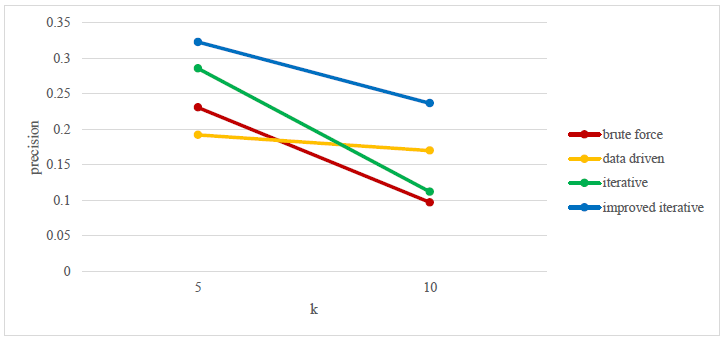
\includegraphics[width=5in]{figures/precision-different-algorithms.png}
    \caption{Precision of augmented tags for different algorithms}
    \label{fig:precision-different-algorithms}
\end{figure}

\begin{figure}
    \centering
    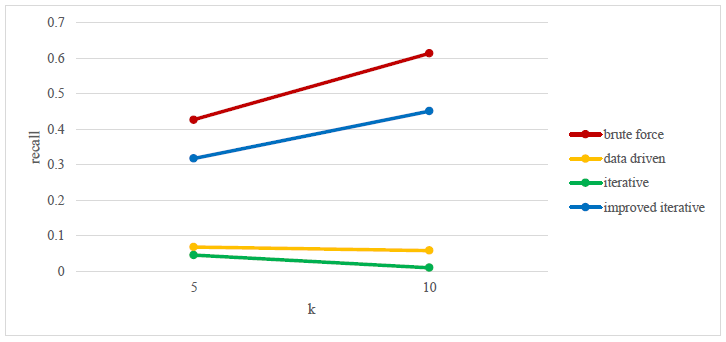
\includegraphics[width=5in]{figures/recall-of-augmented-tags-for-different-algorithms.png}
    \caption{Recall of augmented tags for different algorithms}
    \label{fig:recall-of-augmented-tags-for-different-algorithms}
\end{figure}

\begin{figure}
    \centering
    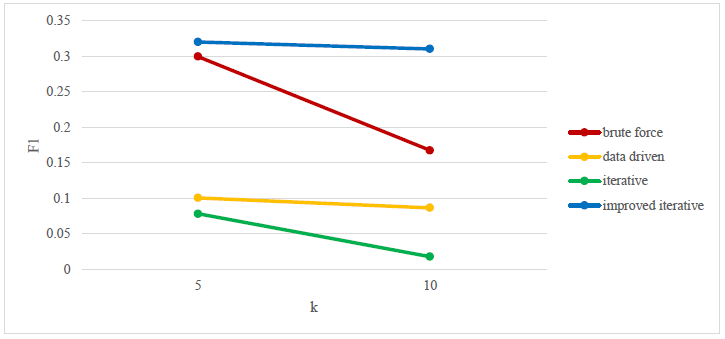
\includegraphics[width=5in]{figures/f1-of-augmented-tags-for-k-tables-in-repository.png}
    \caption{F1 of augmented tags for k tables in repository}
    \label{fig:f1-of-augmented-tags-for-k-tables-in-repository}
\end{figure}

\begin{figure}
    \centering
    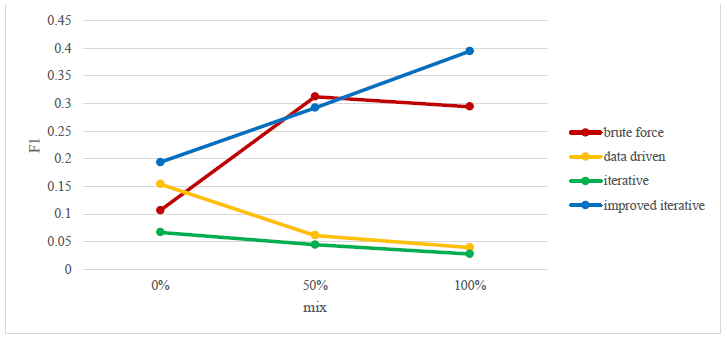
\includegraphics[width=5in]{figures/f1-of-augmented-tags-for-different-mixes-of-tables.png}
    \caption{F1 of augmented tags for different mixes of tables}
    \label{fig:f1-of-augmented-tags-for-different-mixes-of-tables}
\end{figure}

\begin{figure}
    \centering
    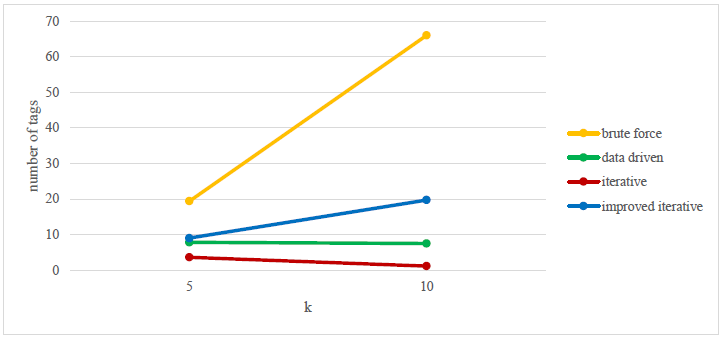
\includegraphics[width=5in]{figures/number-of-new-tags-added-given-k-tables.png}
    \caption{Number of new tags added given k tables}
    \label{fig:number-of-new-tags-added-given-k-tables}
\end{figure}

\begin{figure}
    \centering
    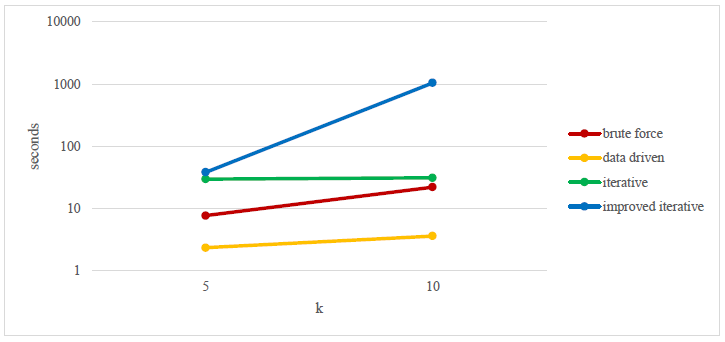
\includegraphics[width=5in]{figures/runtime-of-different-algorithms-for-different-k.png}
    \caption{Runtime of different algorithms for different k}
    \label{fig:runtime-of-different-algorithms-for-different-k}
\end{figure}
%%%%%%%%%%%%%%%%%%%%%%%%%%%%%%%%%%%%%%%%%%%%%%%%%%%%%%%%%%%%%%%%%%%%%%
\section{Experimental results}
\label{sec:ExperimentalResults}

We evaluate our experimental results in this section. For input repository size k = 5, 10 and with Parks as the base table, we perform tests on the 4 algorithms we implemented. All tests are run on macOS 10.14 with the configuration of 1.8 Ghz Intel Core i5 (5350U) and 8 GB RAM. For each repository of size k, we create multiple tests each with a different mix of related and unrelated tables. For example, for k equal to 5, one possible mix is one base table, 2 related tables, and 2 unrelated tables. We measure the accuracy in terms of precision and recall. As a quick measure as opposed to precision and recall, we also measure the number of new tags generated regardless of the correctness of the tags. In addition to accuracy, we also measure the runtime of each algorithm given a specific input. We note that each algorithm with its given input is only run once, but we would like to compute the average of multiple runs (with cross-validation) as future work.

\subsection{Precision and recall}

We measured the four algorithms in Chapter 4: Solutions in terms of precision and recall with different parameters for each test, the results are shown in Table 5-1. The accuracy of Data Driven does not reflect the its actual performance, because it only creates tags for the base table and there is no mechanism for retrieving related tables. We added additional measurements for the accuracy of Improved Iterative after some modifications were made (shown in the last column of Table 5-1). We removed the schema matching step between the attributes in the iterative method. Once a related table is found, its topics are compared to each topic in every partition, if a pair of topics have a high similarity score, the topic and the attribute are added to the partition without schema matching.

For every input size k, we took the average of the accuracy and created a plot in terms of the input size, the plot for precision is shown in \autoref{fig:precision-different-algorithms} and the plot for recall is shown in \autoref{fig:recall-of-augmented-tags-for-different-algorithms}. All four algorithms decrease in precision as the number of tables in the repository increases from 5 to 10. Data Driven decreases precision the least, from 0.19 to 0.17, while Iterative decreases the most, from 0.29 to 0.11. Improved Iterative also decreases precision, from 0.32 to 0.24, but it still has the highest precision at k=10 compared to the other three algorithms. However, when the additional logics are removed, the precision of Improved Iterative is only 0.11 at k=10, which is close to the precision of Brute Force and Iterative.

The recall either increase or decrease as k increases. The recall of Iterative and Data Driven are much lower compared to the other two algorithms, and the recall of both decrease as the number of tables increases. Since the precision of Iterative and Data Driven also decrease, we consider

these algorithms poorly designed. Brute Force and Improved Iterative both increase in recall as the number of tables increases, and there is a tradeoff of precision over recall as the number of tables increases. While Brute Force has the highest recall for both k=5 and k=10, the recall of Improved Iterative is comparable. We note that Brute Force has a much lower precision.
We performed rolled-up of the results in the dimension of k, and computed the average for every mix proportion. The precision is shown in Table 5-2 and the recall is shown in Table 5-3. A well-designed algorithm should not decrease in precision or recall when the proportion of related and unrelated tables change. However, we observe that decreased its precision drastically as the mix shifts from 100% to 0%, this suggests that Improved Iterative requires more improvements for future work.

We then performed rolled-up of the results in both k and mix proportion. Improved Iterative has the highest precision of 0.28 while Brute Force has the lowest precision of 0.16, but Brute Force

has the highest recall of 0.52 while Iterative has the lowest recall of 0.03. We think that Brute Force has a high recall because it blindly adds all tags it finds. The reason that Iterative has a low recall is because it only uses N-gram as the matching criterion, which fails to identify semantically similar tags.
We ranked the four algorithms based on how well they perform for each test. Of the 12 tests, Improved Iterative ranks first 7 times and ranks second 3 times. The only test it performs much worse than another algorithm is for k=10 and the repository contains 9 unrelated tables. We think Improved Iterative cannot correctly reject unrelated tables, and therefore adding too many incorrect tags. The semantic distance is affected by the initialization step, which we may need to improve in the future.
Using the precision and recall, we now compute the F1 score for the four algorithms. The plot for the F1 score at different k is shown in \autoref{fig:f1-of-augmented-tags-for-k-tables-in-repository}. The plot for the F1 score for different mix proportions of related and unrelated tables is shown in \autoref{fig:f1-of-augmented-tags-for-different-mixes-of-tables}.

As k increases, the F1 score for all of the algorithms decrease, but different algorithms decrease at different magnitudes. The F1 score for Brute Force decreases the most, from 0.30 to 0.17,

while Improved Iterative decreases the least, from 0.32 to 0.31. Improved Iterative performs the best for all k. As the mix proportion changes, F1 for each of the four algorithms changes in different ways. Data Driven and Iterative decrease in F1 as the mix proportion increases, while Improved Iterative increases in F1 as the mix proportion increases. Brute Forces F1 increases at 50% but decreases at 100%. Improved Iterative performs the best among all four algorithms.
However, we think a good algorithm should have a constant F1 score regardless of what mix proportion it is given. This suggests again that more improvements needs to be done as future work.

\subsection{New tags added}

We measured the number of new tags added to the augmented metadata for the four algorithms in Table 5-4. Brute Force adds the most number of new tags on average, 42.71 per table, Data Driven adds 7.63 tags per table, while Iterative only adds 2.33 per table. Improved Iterative adds 14.35 tags per table. When additional logics are removed for Improved Iterative, 25.96 new tags are added, this demonstrates that the schema matching step is able to filter out many tags.

Since Brute Force adds every tag from a related table, we can compare other algorithms with Brute Force to estimate the selectivity of the other algorithms. Iterative is highly selective, since there are no new tags added for the test mix = 1+9, either because no related tables are found or none of the tags in the related tables are similar to the base table tags. This outcome is desirable because none of the 9 tables in the repository are related to the base table. Data Driven does not add many new tags either, since there is an upper bound on the number of new tags, which equals to the number of attributes in the base table. Improved Iterative adds more new tags than Data Driven, but less than Brute Force.

The plot in \autoref{fig:number-of-new-tags-added-given-k-tables} shows the average number of tags added as k increases. For Brute Force, the number of tags added per table increases as expected, since there is one or more tags per table on average. For Data Driven, the number of new tags does not change, since the number of attributes in the base table remains constant. For Iterative, as repository size increases, the number of new tags added per table decreases. This is due to the uncontrollable factor that we have different tables between the testing set for k = 5 and k = 10, there are more new tags that Iterative can add for the k = 5 set and there are less that it can add for the k = 10 set. For Improved Iterative, the number of new tags doubles as k doubles, which is a desired result.

\subsection{Runtime}

We measured the runtime for the four different algorithms, and the results are shown in Table 5-5. Each test can be completed within a reasonable timeframe for all of the algorithms. Iterative and Improved Iterative terminated the iterative method in less than 5 iterations (either 2nd, 3rd, or the 4th iteration) for all tests. However, we have not included any tests with more than 10 tables in the repository, and we cannot conclude that any of the algorithms is efficient

We created a plot to show the runtime of each algorithm as the repository size k increases, shown in \autoref{fig:Runtime of different algorithms for different k}. Each value is an average of three tests of different mixes of related and unrelated tables. We observe that Brute Force, Data Driven, and Iterative do not increase in runtime by orders of magnitude, but Improved Iterative increases from 38 seconds to 1042 seconds as k increases from 5 to 10. Empirically, it is likely that the algorithm has exponential asymptotic complexity. We measured the time to enrich attributes and topics of each table in the repository, and the time to enrich 5 tables in around 3 seconds. We also measured the time to perform semantic labeling between attributes and tags, the time is around 15 seconds for 5 tables. Most of the computation time is in the schema matching step in the iterative method. As we removed the additional logics, the runtime drops significantly and the runtime of Improved Iterative is comparable to the Iterative.

We analyzed the theoretical asymptotic upper bound for the iterative method. For n tables, t tags per table, m attributes per table, and assuming the matching criterion make comparisons in O(1), the upper bound of the iterative method is approximately nt(nt*nt + t*nt*(nt+nm)), or O(n3t3+n3t2m). The maximum number of iterations is nt since we add at least one tag to the base table partitions per iteration and will not consider that tag again in future iterations. For each iteration, the table search step makes at most nt*nt tag comparisons. Once a related table is found, the partitioning step for the semantic labels is t*nt*(nt+nm), since there are t candidate tags, nt partitions, and within each partition there are nt tags and nm attributes. Based on the theoretical bound, the iterative method has polynomial complexity.
We removed the schema matching step on the attributes that may have contributed to the increase in runtime, and the complexity of the iterative method is reduced to O(n3t3).

































%    6. Discussion
%% The following is a directive for TeXShop to indicate the main file
%%!TEX root = diss.tex

\chapter{Discussion}
\label{ch:Discussions}

In this thesis, we aim to achieve the goal of finding a common representation of metadata that is easily interpretable, and augmenting tables with additional metadata tags to make the tables more searchable and understandable.

In this chapter, a list of questions we would like to be answered are:
\begin{enumerate}
\item How to make augmentation of topics computationally feasible? How to reduce computation for summarization, schema matching, semantic labelling? In other words, how to scale up in terms of number of tables and table size?
\item How to make the augmented topics adhere more closely to real world scenarios? How to only augment topics that the user is interested in?
\item How concise should the tags and topics be, in order to generate useful metadata?
\item How to develop an approach that generalizes to data instances with different characteristics? Every data instance has its own characteristics, some are easier to work with to generate metadata, while others are not.	
\end{enumerate}

To address the question of how to make augmentation of tags computationally feasible, we would like to revisit the idea of placing the communication step at an early step of the algorithm. By our assumption that each table already contains some useful metadata, and there is a base table to guide how to choose related tables, we developed an iterative approach to discover new information between a large number of tables. Our description of the iterative approach raised the need to find related tables so that we can compare their tags with the base table tags. We proposed to use overlapping of existing tags to approximate relatedness between tables, which reduces the cost of schema matching on the full set of tables each with many attributes in the repository. Computing the tag overlaps between two data instances is simple, but the cost is not negligible when the repository contains too many tables. We intend to replace or improve this costly step as future work.

We also discussed partitioning as an alternative to clustering to find groups of similar attributes or tags. Our implementation of the partitioning step in Improved Iterative is not efficient, and the total runtime of the algorithm is much higher than Brute Force. One reason is that we used additional matching criteria which were omitted in Brute Force. But since Brute Force has an exponential upper bound and Improved Iterative has a polynomial upper bound, we think the benefit of Improved Iterative is only apparent when we have more test sets available.

We also observed that by saving all intermediate computation steps, including the similarity matrix of schema matching and the semantic labels, we saved around one minute of time by reusing them in subsequent test runs.

To address the question of how to make the augmented tags adhere more closely to real world scenarios, we would like to revisit the design of semantic labeling. By performing word sense disambiguation using metadata contexts, we are able to attach semantics to attributes and tags. A machine can then interpret these metadata as if a human is understanding every attribute and tag. Rather than comparing a sequence of characters, a matching criterion can find the semantic distance between words, and we are able to create connectivity within a table metadata by semantic labeling between attributes and tags. In some scenarios, semantics and domain knowledge is not required, because an algorithm does not rely on it. As discussed in \cite{Yu2006Schema}, they only relied on existing links between elements to summarize groups of similar elements, these links do not provide semantics to the elements but can specify how they are related. In \cite{LI200049}, they performed clustering of elements based on data distributions of features without knowing what data they are working with.

A human would naturally try to find relationships as they read data from different sources, they could then group similar items together or discover their differences. In the same way, we use multiple matching criteria to determine similarity and differences between attributes and tags from different sources. By creating a partition for a group of similar attributes and tags, we are able to access them all at the same time, and discover new information between the attributes and tags. In our case, we know from which data instance each attribute comes from, and whether every data instance uses the same tag to describe its data. A human tends to only extract information that he or she finds useful, and any incorrect information may be tolerable as long as there is enough information extracted. In the same way, we augment the metadata in a pay-as-you-go approach, such that only data related to a base table is extracted from a repository. It is possible that the iterative method finds some incorrect metadata, but the quality of metadata can be improved over time as more information becomes available. A user may also prefer to choose whether to maximize precision or recall in the augmented metadata. Although both are important for a high quality output, it is difficult to achieve both. It is possible to let a user specify whether precision or recall is desired in a schema matching output before the algorithm is run \cite{Duchateau2009YAM}. Their algorithms would then adjust to meet the user's preference.

To address the question of how concise the tags and topics should be in order to generate useful metadata, we revisit the idea of summarization and its computational complexity. We first limited the vocabulary of the tags to reduce computation costs, no new tags are generated when an algorithm is run. We also made sure that by the end of an algorithm, all the related tables have reached a consensus on the tags representation (all the related tables have a same set of tags). The common representation permits a user or a program to search and filter by these tags. We may also relate the layout of our metadata to an autoencoder \cite{kipf2017semisupervised}, where the tags are the hidden layer in the neural network. This hidden layer is initially meaningless, but as we observe more data, the tags start to reach a common representation that can correctly represent similarities between the tables (and the attributes). We argue that the tags play an important role in many common complex problems. By creating a common representation of tag words that machines can understand, and process these words just like symbols without the need to understand the semantics.

We are unable to address the fourth question since we have not experimented on non-tabular data. However, we note that we can always create abstractions and break down large problems into smaller tasks, list a number of existing methods that were used to study other problems that can solve our tasks, and identify the changes that need to be made to solve our tasks. For each type of data, users usually tackle their problem from an engineering perspective, and explain how metadata augmentation works for their own data. However, we encourage users to think how to convert their data to tabular format, just like how we converted JSON data to CSV format. They are then able to reuse our algorithms by only making small changes.

%%%%%%%%%%%%%%%%%%%%%%%%%%%%%%%%%%%%%%%%%%%%%%%%%%%%%%%%%%%%%%%%%%%%%%
\section{Discussion of the iterative approach}
\label{sec:DiscussionOfTheIterativeApproach}

\subsection{Semantic enrichment discussion}

As a future extension, instead of only attaching the definition of a word, a more robust way is to attach all of its synonyms. In \cite{Giunchiglia2005Semantic}, words of each attribute name are enriched with all of its synonyms and these synonyms are connected through disjunctions. Such attachment allows the authors to perform logic programming. Since every Lemma in a Synset are synonyms of each other, we should be able to create a context for a word using information of the synonyms in addition to the information of the word itself.

Words in WordNet can be organized into a hierarchy, where hypernyms of a word are located above the word in the hierarchy. These hypernyms are the parents of the word. On the other hand, a word can be the hypernym of other words. Then these other words are the daughters of the hypernym. The sisters of a word are located in the same level in the hierarchy and share a common parent. We note that synonyms of a word can be the daughters or sisters of the word, and we may run into the issue of adding too much unrelated information of the synonyms to the context. In data exploration literature \cite{10.14778/3021924.3021935}, two modalities of drilling down data are horizonal and vertical. Horizontal exploration explores data that are the sisters, and vertical data exploration explores data that are the daughters. For example, one sense of the word $park$ is \textit{`a piece of open land for recreational use in an urban area'}. Its synonyms are commons and green, and they could be the sisters or the daughter of park. They argued that more related information are found by exploring the daughters than in the sisters. We therefore leave the experiment of adding synonyms as future work.

As another improvement, we can include adjectives to the context because overlaps in adjectives may also contribute to word sense disambiguation. We also intend to count the number of non-overlapping words, and select the word sense with the least number of non-overlapping words. The impact of selecting non-overlapping words will also be assessed as future work.

\subsection{Semantic labeling discussion}

We explain how semantic labeling is related to existing data integration techniques. In our work, since a tag can be shared across multiple tables, all the tags act like a mediated schema, where we use semantic labeling between metadata tags and schema attributes to maintain the semantic similarity across different tables. The semantic labeling acts as a source description. Assuming that there is a mediated schema that contains all possible mediated attributes, it is then easier to integrate all the schemata together. Integrated data also allows one to ask questions on a global mediated schema without the need to understand the individual local schemata.

An application of using mediated schema in matching was proposed \cite{DBLP:journals/pvldb/ChanialDGLNM18}, they used an attribute dictionary to perform instance matching. The dictionary is a knowledge base that stores attributes and its representative values, as well as probabilities of these values. The final matching between a pair of tables is determined transitively through the dictionary. The matching between a pairs of elements involve matching to the dictionary first, then an algorithm for solving the max-flow problem was used to find the best matching.

\subsection{Table search discussion}

The main idea of table searching to reduce the search space. Techniques that can reduce the search space include source selection \cite{Dong2012Proceedings}, partitioning \cite{Moawed2018Arabian}, and blocking \cite{Mudgal2018Deep}. In source selection, each table in the repository is retrieved one-by-one or in small batches, in the order from the most similar to the least. Partitioning place similar pairs of elements into the same partition, and perform further operations at each partition separately \cite{10.1145/1066157.1066283}. Blocking is a technique to reduce the number of comparisons, by eliminating pairs of elements that are highly dissimilar in the early stage \cite{Ehrig2004QOM}.

We only used source selection to reduce the search space. One of the challenges for table search is that the order in which a table is selected affects the quality of the matching, especially if only a small subset is selected. A similar issue has been addressed in \cite{Dong2012Proceedings}. In previous works, for sources with overlapping information, greedy algorithms were proposed to answer queries \cite{10.1145/1951365.1951414}. These algorithms greedily select sources, and return approximate answers quickly. There are also tools that produces a ranked list of schema in decreasing order of relatedness to the query table \cite{DBLP:conf/sigmod/ChenMH09}. In our case, if the greedy algorithm is ineffective, and the selected candidate tables are unrelated, we are unable to find the right metadata tags to augment. Since relatedness is typically approximated, and do not necessarily reflect the true relatedness, we need to make sure that our measure of relatedness is close enough to the true relatedness. We also mentioned that the table search we implement is done in an iterative manner, which reduces the chance of missing related tables, which we will explain in our main algorithm in \autoref{sec:IterativeApproach}.

\subsection{Partitioning discussion}
\label{ssec:PartitioningDiscussion}

There is a number of advantages of partitioning over clustering. When hierarchical clustering is performed, each attribute can only appear in one cluster. When we perform partitioning, it is possible to assign an attribute to multiple partitions. When we allow an attribute to be assigned to multiple partitions, similar partitions contain similar attributes (and thus indicating that the two partitions should be merged). Assigning an attribute to multiple partitions overcomes the limiting constraint discussed in \autoref{ssec:UsingSchemaMatchingOnOpenData}, so that now each attribute can be labeled with multiple tags. Furthermore, partitioning will save computation time, since every attribute-to-topic label is only examined once, unlike clustering where multiple iterations are needed.

One advantage of clustering over partitioning is that it allows a holistic view of all schemata at the same time. By performing multiple iterations of comparisons, clusters can change composition, whereas partitioning is only done in one iteration and comparisons are at a limited scope.

As an extension of the current partitioning method, we can merge or split partitions if needed, but we leave these operations as future work. If there is enough evidence that two partitions are highly similar, then we can merge them. On the other hand, if we discover that there are two or more distinctive groups of attributes in a partition, then we split the partition. We also note that when the semantic labeling is incorrect, the attribute is labeled with a wrong tag, then we need additional procedures to find the correct partition for the attribute. We will briefly revisit this idea when we discuss our main algorithm in \autoref{ssec:FutureWorkForTheAlgorithm}.

When only attribute-to-attribute correspondences is provided, an alternative approach to clustering is to perform schema merging \cite{Pottinger2008Schema}, where we take the union of all the correspondences using the known attribute overlaps to generate a mediated schema. We can then use the generated mediated schema to create topics, and semantic labeling.

We next discuss summarization and how it relates to partitioning. In a summary generation problem, complex and scattered data (such as unstructured text) is summarized and presented in a more compact and organized format (such as a list of topic words). When data is stored in a more organized format, such as tabular data. A table column can contain numeric values, symbols, acronyms, symbols describing a state or a classification, or sentences. Since tabular data is more discrete in nature, we cannot use the summary generation methods on natural language.

Many methods were invented for specific data domains and formats, and many generalized methods were also invented for understanding and organizing data in any domain \cite{Park2015Evaluation}. We made the assumption that we already know what types of metadata the user considers interesting, in our case, it is the tags in each data instance. Therefore we leave the generalized method as future work, and as we have limited the scope of our study, we only use existing tags in the open data repository as the summary of data instances. When we perform partitioning of the attributes and topics, we place similar items in the same partition, and the resulting partitions become the summary after we choose one representative example from each partition. The partitions are then used to create the semantic labeling as our algorithm output, which we will explain in \autoref{ssec:FromPartitionsToMetadataTags}. We also note that in \cite{Diego2018Machine}, the algorithm outputs both the schema matchings as well as an additional ontology. The ontology is able to provide more context to the user to understand the matchings. In our case, the output semantic labeling from our algorithm can immediately be transformed to the summary metadata tags, and the tags is intuitive for the user to understand.

\subsection{Future work for the algorithm}
\label{ssec:FutureWorkForTheAlgorithm}

The iterative approach uses the base table to find other related tables, and relatedness of tables are assessed by tag overlaps. After one table is compared with the base table and tags are added to the partitions, the next table selected related table can have tag overlap with either the original base table tags or the newly added ones. This is because we update the base table state $S$ to include the newly added tags. At the end of the iterative method, the base table as well as all the related tables are augmented with tags. We are able to achieve this because we keep track of which table an attribute is from, and we also keep the attribute-tag semantic labeling created during the initialization step, knowing both allows us to add back the augmented tags to the table.

The initialization step produces a set of semantic labels, where each attribute is labeled zero of more tags, and it is possible to transfer the tags back to the tables without running the iterative method. But we cannot be sure that these tags are correct, since the semantic labeling created are mappings between attributes and tags within one table only, it is not certain that a tag used in one table is also used for the same purpose in another table. There is no knowledge of which tables contain these tags and how the tables use the tags to describe the data. We may also miss many tags due to the limited power of semantic labeling, this justifies the need of table search, where we find tables sharing common tags, and extend with additional tags that were not already in each table. Unlike Data Driven, which can only augment a limited number of new tags, this approach can augment as many tags as possible. We need to perform schema matching to allow each table to communicate with other tables and verify whether all the tables agree with the tags vocabulary.

The iterative method replaces the full-scale schema matching done by Brute Force, reducing the total computation time of augmenting metadata. Schema matching to compare between every pair of attributes between each pair of tables is reduced to only comparing the base table with its related tables. Instead of matching attributes between schemata immediately, we compare the tags from the semantic labeling first. We use the tags as the mediator to find similar attributes, because the number of tags is often less than the number of attributes, and the tags is from a controlled vocabulary which is more representative than the attributes. In \cite{Moawed2018Arabian}, the initialization involves computing a LSH hashing index, and their table search uses this index to quickly locate similar set of attributes from tables, which allows them to compare these attributes. Compared to our initialization step and table search, we are also trading off correctness for speed. But we argue that the semantic labeling created from metadata tags increase the recall and precision of the augmented tags, even though we did not perform full-scale schema matching. During table search, we use tags to guide which pair of tables to compare, after adding related tags to the base table partitions (which increase precision), we then use these tags to find more similar tables in an iterative manner (which increase recall) until there are no more tag overlaps.

The iterative method terminates because we remove the tags (added to the base table partitions) from the selected related table during each iteration. We do not intend to select the same tables in future iterations because of the same tag overlaps, if the same tables are found to be similar in a future iteration, it is because of tag overlaps for tags not already added to the base table partitions. To give an example, tables $A$ and $B$ are found to be unrelated in an early iteration due to the lack of tag overlaps, but after more tags from table $C$ are added to $A$ in a later iteration, tables $A$ and $B$ are now found to be related because of the tag overlap between the new tags added from $C$, which $B$ shares. As the number of tag overlaps decreases between the base table and any table from the repository, the iterative method terminates once no more related tables can be found. Numerous termination conditions can be implemented as future work, such as terminating because no new tags or too few tags are added in the last iteration. In \cite{Nargesian2018Table}, they ended table search when $k$ tables are found, we can terminate in a similar way when $k$ new tags are added to the partitions. We can also terminate because a specified maximum number of iterations is reached.

We will improve the Partition step as future work as described below. The purpose of the iterative method is to make incremental changes at each iteration, and when it terminates, the incorrectness left in the partitions is minimized. We should first be able to remove a tag from a partition if it does not belong in that partition. For example, \textit{Park} has mistakenly added \textit{infrastructure} to one of its partitions, but we later find that the tag \textit{infrastructure} is used in a different context as seen in \textit{DrainageCatchBasins}, because \textit{DrainageCatchBasins} contains the tag in its original metadata whereas \textit{Park} does not. We should then remove the \textit{infrastructure} tag from the partitions. Similarly, we need to remove attributes from a partition when an attribute that was added previously no longer belongs in the partition as additional attributes are added. By SchemaMatching, we can also determine if there are any attribute not similar to the other attributes in the partition. The second operation in the improvement is splitting of a partition. We can perform clustering within a partition to find two or more groups of distinct tags, and we can split the partition based on the groups. However, the choice of a clustering algorithm to use is yet to be determined. We can similarly add a merge operation. The third improvement is to add an attribute not mapped with any tags to a partition. We compare the attribute with every attribute in every partition to find a suitable partition for the attribute. However, we think all of the above operations require additional number of comparisons with attributes and tags, and we need to find efficient algorithms to achieve these operations. One possible improvement is to avoid comparisons between every pair of items in a partition when an attribute or a tag is to be added, we compare with a representative example in the partition instead.

We also propose improvements for SchemaMatching within the iterative methods. We propose to add two measures, \textit{importance} and \textit{coverage}, to assess the similarity of a candidate tag. Importance is a measure for how many attributes are mapped with the candidate tag. In the case of comparing a base table with a related table, if many attributes in the base table can be mapped with the related table candidate tag, then the tag has high importance. We can decide to create a new partition for the candidate tag. Coverage is a measure for the number of partitions that the candidate tag could be placed in. If many tags from different partitions are similar to candidate tag, then it has high coverage. We can unconventionally decide to add the tag to multiple partitions. Other improvements of SchemaMatching include adding additional matching criteria to improve the quality of the similarity scores.

\subsection{Future work for the improved algorithm}

The FastText schema matching criterion is inadequate for computing similarity scores. We quickly compared the performance of FastText with WordNet, and found that WordNet is more likely to output true positives. Thus we used WordNet for both word sense disambiguation and schema matching and did not use word vectors to compute semantic distances.

As an extension, we can add additional schema matching criteria to provide additional evidence for accepting or rejecting a pair of items. We would like to add an extension to WordNet, where we use domain-specific knowledge bases or ontologies to perform word sense disambiguation and to find semantic distance between pairs. An ontology helps identify existing relationships among attributes and tags, because each concept has properties, and we can verify the semantic distance between concepts by the similarity of their properties. However, this work needs to be done collectively by many data experts. In \cite{Sorrentino2011NORMS}, they faced the issue of too many acronyms, abbreviations, or out-of-vocabulary words in their data. They performed normalization of the words by looking up knowledge bases available on the Internet, and replaced the words in question with known words.

Another matching criterion we may use is instance-level matching. When comparing a pair of attributes, we compare the column values each containing a list of unique values. We can then adopt the approach in \cite{Nargesian2018Table} to find attribute unionability. To speed up comparison, we can aggregate all the unique values of an attribute $A_s$ into a document and compare a pair of documents using NLP techniques discussed in \autoref{ssec:VariationsOfSchemaMatching}. For example, we can combine the values [\textit{`HartnellPark',`BettyHuffPark',`BlackieSpit',\ldots}] into\\ \textit{`HartnellPark,BettyHuffPark,BlackieSpit,\ldots'}, and compare it with another document. However, most NLP techniques relied on the sentence structure within documents, and these techniques are less powerful for our data due to the lack of full sentences in the column values.

%%%%%%%%%%%%%%%%%%%%%%%%%%%%%%%%%%%%%%%%%%%%%%%%%%%%%%%%%%%%%%%%%%%%%%
\section{Future work for experiments}
\label{sec:FutureWorkForExperiments}

Many experiments that we intend to perform are left as future work. We would like to give more analysis to why Improve Iterative has a high runtime. To achieve this, we monitor the progress of each iteration in the iterative method, and measure the accuracy and runtime after each iteration. We would also like to the measure the four algorithms with tests of larger $k$, use a variety of tables as the base table, and evaluate for different domains other than the park domain. We also need to create the gold standard for these different domains.

We noticed that many of the tags augmented by an algorithm are not present in the gold standard, but some tags are somewhat related to the base table. We could choose to add these somewhat related tags in the gold standard and rerun our test. But we could also choose to incorporate these tags into the accuracy calculation. We find the semantic distance between these somewhat related tags and the tags in the gold standard, take the maximum distance score between a pair, and add the score towards the accuracy of the test. We expect the precision to increase for all algorithms.

We only performed offline evaluation, but a good evaluation method needs to measure both the humans ability to understand the data and machine's ability to interpret the data. By performing offline evaluation, we only addressed machine interpretability. We will address the goal of improving human's ability to understand the augmented tags via user studies. We provide the repository, the tags, and a questionnaire to a number of participants, and assess their ability to answer the questions about the data when augmented tags are provided.

%%%%%%%%%%%%%%%%%%%%%%%%%%%%%%%%%%%%%%%%%%%%%%%%%%%%%%%%%%%%%%%%%%%%%%
\section{Usefulness of augmented metadata tags}
\label{sec:UsefulnessOfAugmentedMetadataTags}

Augmented metadata provides more interpretability to the tables through a common representation shared between multiple tables. For example, the tags in \autoref{fig:example-park-specimen-trees} were augmented, and the augmented set is shown in \autoref{fig:augmented-park-specimen-trees}. The tag overlap between \autoref{fig:example-parks} and \autoref{fig:augmented-park-specimen-trees} becomes [\textit{parks, environment, green, and nature}]. After we increase the tag overlaps between metadata of tables, searching, filtering, and explaining becomes easier for the user and machine programs.

When performing searching for similar tables, the user provides a list of tags as the query, and compare each table in the repository. The metadata of each table is compared with the query, if there are many tag overlaps between the query and the metadata of the table, then it is highly likely that the table instance contains information the user wants. For example, if the user provides \textit{parks} OR \textit{trees} as the query, then the metadata in \autoref{fig:example-parks} overlaps in [\textit{parks}] and the augmented metadata in \autoref{fig:augmented-park-specimen-trees} overlaps in [\textit{parks, trees}]. The two tables now overlap in [\textit{parks}], whereas the original metadata in \autoref{fig:example-park-specimen-trees} only overlaps in [\textit{trees}] and the two tables overlap in nothing. When performing filtering, the query becomes \textit{parks} AND \textit{trees}, and the table in \autoref{fig:augmented-park-specimen-trees} is in the results while the table in \autoref{fig:example-park-specimen-trees} is not. Finally, the augmented metadata can also help explain what information the table contains. We first examine the metadata of a table, and compare it with metadata of another table. If the two tables share many similar tags, then it is highly likely that they also share many similar data. When a user sees the augmented tags in \autoref{fig:augmented-park-specimen-trees} and \autoref{fig:example-parks}, the user can understand that both tables store information related to \textit{parks} in the urban area.

%%%%%%%%%%%%%%%%%%%%%%%%%%%%%%%%%%%%%%%%%%%%%%%%%%%%%%%%%%%%%%%%%%%%%%
\section{Augmented metadata helping other problems}
\label{sec:AugmentedMetadataHelpingOtherProblems}

We discuss a number of downstream data management tasks that benefit from our augmented metadata tags, with the focus on how topic extraction can help speed up data integration. High-quality augmented tags for each table are helpful in an end-to-end data-to-knowledge pipeline. In a data warehouse ETL pipeline, users and machines can easily consolidate related data instances by using tags to search tables and filter tables, and perform operations on the tables that are related to each other in the result of search. Data lakes are storage systems that simply store the data without thinking about the data being stored. There are existing works on preprocessing the data, identifying anomalies, before the data is stored. If tags are available for preprocessing, then they can help detect semantic similarities between data instances, and help grouping similar data together before storing them. In data integration, users can more easily create mediated schema for a repository of heterogenous schemata if they can use tags to group similar tables together, and create mediated attributes for each group of related attributes.

As we have mentioned, the augmented metadata tags are a summary of the data instance. But we have not considered finding the smallest set of tags that can describe the data instance well. Let the set of metadata be \textit{Parks(environment, green, nature, parks), ParkSpecimenTrees(trees, parks, environment), ParkScreenTrees(parks)} and \textit{DrainageCatchBasins(devices, infrastructure)}. Suppose the following pairs of tags are highly similar: \textit{environment} and \textit{nature}, \textit{green} and \textit{trees}, \textit{parks} and \textit{environment, parks} and \textit{trees}, and \textit{devices} and \textit{infrastructure}. Using our iterative approach, we would be placing similar tags in the same partition. We can then select one tag from each partition, and let these selected tags be the summary. For example, one possible summary is [\textit{parks, environment, trees, and infrastructure}].

During semantic enrichment, we have attached a Wordnet definition to each attribute and tag. The Wordnet definition allows disambiguation between homonyms having different senses. We can then integrate these attributes and tags to an ontology, and let the ontology be the metadata for the data instance. Each attribute or tag serves as a concept in the ontology, and its Wordnet definition becomes a property of the concept. Using the semantic distances between concepts, relationships can then be created. If we have enough tags to describe a data instance and know the rich interlinkages between the tags, then the ontology can substitute the data instance itself, because the ontology could be more machine-understandable and human-readable compared to the data instance.

Ontologies allow a different way of integrating data called publish-time data integration, where the data author needs to figure out the semantic overlaps of the new table with every possible existing table in the repository \cite{Diego2018Machine}. The publish-time approach contrasts with the pay-as-you-go approach in that the former pushes new data to a repository, and the latter pulls information from the repository to enhance the table that the user keeps locally. But with tag overlaps, the user could find semantic overlaps with less effort.

%%%%%%%%%%%%%%%%%%%%%%%%%%%%%%%%%%%%%%%%%%%%%%%%%%%%%%%%%%%%%%%%%%%%%%
\section{Future improvements and extensions}
\label{sec:FutureImprovementsAndExtensions}

We have already discussed various ways we can improve our work throughout this thesis, and we will not repeat them here. We will raise only one idea that we have not discussed previously. Instead of returning one answer, an increasingly popular alternative is to return multiple answers and let the user choose which answer he or she needs. In \cite{ilprints851}, where they constructed a data integration system in a pay-as-you-go fashion, they returned a set of possible answers each with a probability attached. They relied on schema matching to create the mediated schema for the heterogeneous schemata, created a graph of attribute correspondences, and then clustered the attributes. Given the one-to-one cardinality constraint, they created different versions of the mediated schema, each with some differences in what mediated attributes are in the mediated schema and how the attributes are mapped to the mediated attributes. Using the schema matching scores between the attributes, they computed a probability for each possible mediated schema. We can adopt a similar approach to return a set of possible answers, where in each answer we augment tables with slightly different set of tags. For example, if a tag is placed in multiple partitions, and given a constraint that a tag can only be in one partition when augmenting the tags, we can create different versions of the augmented tags.

%%%%%%%%%%%%%%%%%%%%%%%%%%%%%%%%%%%%%%%%%%%%%%%%%%%%%%%%%%%%%%%%%%%%%%
\section{Limitations in our approach}
\label{sec:LimitationsInOurApproach}

We have talked about the limitations of the algorithms we designed throughout this thesis, and we will not repeat them here. We would like to revisit one assumption that we made in \autoref{sec:ScopeOfImprovingMetadata}, where the user does not require the completeness of the metadata they see, and it is okay to create the augmented metadata in a pay-as-you-go fashion. We would like to relate our assumption to the open world assumption made in a data integration setting \cite{Doan2001Reconciling}. The assumption states that the answers returned by queries on data integration systems is not complete, since they do not know if there are other unintegrated sources that contain additional data. As long as the answer is consistent with respect to the existing subset of data, the user should be okay with the incompleteness. Given that our scenario is similar to theirs, we also make the open world assumption and give our best effort at augmenting metadata for each table.

%%%%%%%%%%%%%%%%%%%%%%%%%%%%%%%%%%%%%%%%%%%%%%%%%%%%%%%%%%%%%%%%%%%%%%
\section{Related areas not addressed by metadata augmentation}
\label{sec:RelatedAreasNotAddressedByMetadataAugmentation}

We describe a number of related areas of research, and list the differences between the problems they solved and the problem we aimed to solve. An area of study in information retrieval is query answering, where the goal is to either return a precise or approximate answer (containing specified data in the tables) to a query. We did not address query answering because we only augmented the metadata without considering how a query can be answered using the data and metadata. In our iterative approach, the table search step answers the query of finding all tables related to a given table. Once we have augmented tags for tables, a simple query is to provide a list of tags to find all tables having these tags, which we can implement easily and assess the performance. But if a query is to precisely find all data in a database that satisfy a constraint, then we cannot answer the query trivially.

Within the study of information extraction, we only addressed the problem of inducing additional information using some existing information as seed. When we have tables and metadata as input, we did not create knowledge from raw data such as logs and sentences, we only improved the quality of the existing metadata. We discovered information from a pool of poorly maintained data and metadata exhibiting semantic heterogeneity. By our studies, we aimed to bridge the gap between schema matching, the study of structured data, and natural language processing, the study on unstructured data. Schema matching performs very little information extraction, but we applied more natural language processing techniques to improve the power of schema matching. At the same time, our end goal of augmenting topics resembles more to one of the goals of natural language processing. The algorithm we implemented meets this goal. By word sense disambiguation, we are able to perform schema matching more easily, which formally operated on the data, and the postprocessing at the end of the algorithm reaches the goal of augmenting metadata.

Knowledge graphs and ontologies both represent relations between individuals in the form of triples, very much like the correspondences we created in schema matching. However, the difference is that they have probabilistic information that define distributions over some structure (such as Markov logic networks), and they can perform inference on the graph with a given weighted formulae. The way that they built this graph is by entity resolution to resolve semantic uncertainty in some unstructured text, where they used different ways to collect evidence and make decisions.

We are also unable to address the task of joining tables. Once the user examines the augmented metadata and all the tables retrieved, the next task naturally is to join the tables in order to gain more insight to all of the data. Existing works on table joining aims at foreign key discovery \cite{Song2018GeoFlux}. We argue that knowing about more tags and the tag overlaps can somewhat help discover foreign keys in tables. Suppose that joinable attributes happened to be mapped to the same tag (as determined by the semantic labeling between attributes and tags), it is then possible to discover joinable attributes. However, existing works such as \cite{10.1145/3299869.3300065,10.14778/2994509.2994534} discovered joinable attributes by examining the table values only, and we do not think semantic labeling can perform better than their approach.

Lastly, we must make one distinction between schema matching, which we utilized in our work, and schema mapping \cite{Zhang2018Managing}. A matching identifies the correspondences, while mapping uses the correspondence information to produce instance-level transformations. A mapping typically occurs in a data warehousing pipeline, and involves writing a program to transform input data to output instances, guided by the rules of semantic correspondences. A program that merges two schema would transform elements in the source into elements in the merged schema, and add all entities to a new data instance. For example, if one source contains data \textit{['1']} while another source contains data \textit{['one']}, the transformation \textit{\{'1'-\textgreater 1,'one'-\textgreater 1\}} would transform data in both sources to $1$ and store them in a new data instance. In our work, we only performed schema matching.
\endinput

%    7. Conclusion
%% The following is a directive for TeXShop to indicate the main file
%%!TEX root = diss.tex

\chapter{Conclusion}
\label{ch:Conclusion}

Data in the modern computing landscape needs to be managed by multiple users, and the complexity of data schema has grown to an extent that no single user can understand every detail. When a user needs to understand data not managed by him or her, we proposed attach semantics-rich metadata (especially the metadata tags) to each separate data instance, which serves as a summary of the data. We first reviewed a number of works related to data summarization, searching data, and comparing data by matching, we then discussed how the metadata tags with enriched semantics provide more evidence and context to these works. We aimed to solve the issue of incompleteness in a repository containing open data, and then developed an iterative approach that augments the metadata of tabular data in open data. We made assumptions that allow us to augment metadata in a pay-as-you-go fashion, where we only augmented tags for tables related to a given base table. We showed that our algorithm outperforms baseline algorithm, but also indicated many areas we still need improvement as future work.

\endinput

%   Bibliography
\begin{singlespace}
\raggedright
\bibliographystyle{abbrvnat}
\bibliography{biblio}
\end{singlespace}

\appendix
%   Appendices (including copies of all required UBC Research
%       Ethics Board's Certificates of Approval)
%\include{reb-coa}	% pdfpages is useful here
\chapter{Evaluation data sample}

\section{Test Set}
\label{sec:TestSet}

The example below shows an input test set for evaluating the accuracy of a metadata augmentation algorithm. Each test is configured by a repository size $k$ and a specific mix proportion (e.g., “5+0”), as well as a base table. The first table in a test is the base table (e.g., “parks” for the “5+0” test). Please refer to Surrey Open Data for the data and the metadata in each table.

\lstset{
    string=[s]{"}{"},
    stringstyle=\color{blue},
    comment=[l]{:},
    commentstyle=\color{black},
}
\begin{lstlisting}
{
  "5+0": [
    "parks",
    "park specimen trees",
    "park screen trees",
    "park outdoor recreation facilities",
    "park structures"
  ],
  "3+2": [
    "parks",
    "park outdoor recreation facilities",
    "park sports fields",
    "water assemblies",
    "road row requirements downtown"
  ],
  "1+4": [
    "parks",
    "water utility facilities",
    "sanitary lift stations",
    "drainage dyke infrastructure",
    "water meters"
  ],
  "10+0": [
    "parks",
    "park paths and trails",
    "park natural areas",
    "park specimen trees",
    "park unimproved parkland",
    "park outdoor recreation facilities",
    "park sports fields",
    "park structures",
    "trails and paths",
    "walking routes"
  ],
  "5+5": [
    "parks",
    "park paths and trails",
    "park natural areas",
    "park specimen trees",
    "park unimproved parkland",
    "heritage sites",
    "aquatic hubs",
    "water fittings",
    "road row requirements downtown",
    "water valves"
  ],
  "1+9": [
    "parks",
    "drainage dyke infrastructure",
    "sanitary lift stations",
    "water utility facilities",
    "water valves",
    "water meters",
    "sanitary nodes",
    "heritage routes",
    "water assemblies",
    "aquatic hubs"
  ]
}
\end{lstlisting}

\section{Gold Standard}
\label{sec:Gold Standard}

The example below shows all the related tables in a gold standard for a test set. If a test repository contains many unrelated tables, these tables will not be in the gold standard (nor their tags).
\lstset{
    string=[s]{"}{"},
    stringstyle=\color{blue},
    comment=[l]{:},
    commentstyle=\color{black},
}
\begin{lstlisting}
{
  "5+0": [
    "parks",
    "park specimen trees",
    "park screen trees",
    "park outdoor recreation facilities",
    "park structures"
  ],
  "3+2": [
    "parks",
    "park outdoor recreation facilities",
    "park sports fields"
  ],
  "1+4": [
    "parks"
  ],
  "10+0": [
    "parks",
    "park paths and trails",
    "park natural areas",
    "park specimen trees",
    "park unimproved parkland",
    "park outdoor recreation facilities",
    "park sports fields",
    "park structures",
    "trails and paths",
    "walking routes"
  ],
  "5+5": [
    "parks",
    "park paths and trails",
    "park natural areas",
    "park specimen trees",
    "park unimproved parkland"
  ],
  "1+9": [
    "parks"
  ]
}
\end{lstlisting}

Each of the related tables in the gold standard contains an augmented set of tags. We give the set of tags for one table below.

\begin{description}
\item[Table name:]\textit{Park specimen trees}
\item[Original tags:][\textit{trees}]
\item[Augmented tags:][\textit{status}, \textit{donation}, \textit{park}, \textit{parkland}, \textit{location}, \textit{road}, \textit{residential}, \textit{facility}, \textit{green}, \textit{commercial}, \textit{environmental}, \textit{service}, \textit{trees}, \textit{parks}, \textit{facilities}, \textit{classification}]
\end{description}
\endinput

\backmatter
%    Index
% See the makeindex package: the following page provides a quick overview
% <http://www.image.ufl.edu/help/latex/latex_indexes.shtml>


\end{document}
\endinput

%TODO Committee page